% =============================================================================
% Terminal Failure Is Not Computational Failure:
% A Pre-Collapse Readout Regime in Nonlinear Dynamical Learners
% NeurIPS 2026
% =============================================================================

\documentclass{article}

% NeurIPS 2026 style
% No option  = anonymous submission with line numbers (use this for submission)
% [preprint] = arXiv / non-anonymous preprint (no line numbers)
% [final]    = camera-ready (fill in \author{} block below)
\PassOptionsToPackage{numbers,compress}{natbib}
\usepackage[preprint]{neurips_2026}
% NOTE: neurips_2026.sty already loads: natbib, geometry, lineno, times fonts

% Core packages (load before hyperref)
\usepackage[utf8]{inputenc}  % allow utf8 source
\usepackage[T1]{fontenc}     % use 8-bit T1 fonts
\usepackage{courier}         % use scalable Type 1 monospace fonts
\usepackage{amsmath,amssymb,amsfonts}
\usepackage{mathtools}
\usepackage{amsthm}
\usepackage{graphicx}
\graphicspath{{figures/}}
\DeclareGraphicsExtensions{.png,.pdf}
\usepackage{booktabs}        % professional tables
\usepackage{multirow}
\usepackage{xcolor}

% Cross-referencing (load after amsmath)
\usepackage{hyperref}
\hypersetup{hidelinks,
  pdftitle={Terminal Failure Is Not Computational Failure: A Pre-Collapse Readout Regime in Nonlinear Dynamical Learners},
  pdfauthor={Rohan Maskrey}}
\usepackage[capitalize,noabbrev]{cleveref}

% Figures and algorithms
\usepackage{algorithm}
\usepackage{algorithmic}
\usepackage{subcaption}
\usepackage{wrapfig}
\usepackage{float}   % provides [H] forced placement
\usepackage{placeins} % keep figures within their intended subsection

% Theorem environments
\newtheorem{theorem}{Theorem}
\newtheorem{proposition}[theorem]{Proposition}
\newtheorem{lemma}[theorem]{Lemma}
\newtheorem{corollary}[theorem]{Corollary}
\newtheorem{definition}[theorem]{Definition}
\theoremstyle{remark}
\newtheorem{remark}[theorem]{Remark}

% Custom commands
\newcommand{\R}{\mathbb{R}}
\newcommand{\C}{\mathbb{C}}
\newcommand{\E}{\mathbb{E}}
\newcommand{\bz}{\mathbf{z}}
\newcommand{\bx}{\mathbf{x}}
\newcommand{\bW}{\mathbf{W}}
\newcommand{\bU}{\mathbf{U}}
\newcommand{\grace}{\textnormal{\textsc{Grace}}}
\newcommand{\sr}{\rho(\bW)}

\title{Terminal Failure Is Not Computational Failure:\\
A Pre-Collapse Readout Regime in Nonlinear Dynamical Learners}

\author{Rohan Maskrey\thanks{Code and saved results:
  \url{https://github.com/maskrys-dev/terminal-failure}.} \\
  \texttt{rohanmaskrey@dunelm.org.uk}}

\begin{document}
\raggedbottom

\maketitle

\begin{center}
\small
\textbf{Acknowledgements.} \textit{Standing on the shoulders of giants}
\\ I thank Oneirix LLC for providing compute.
\end{center}

% =============================================================================
% ABSTRACT
% =============================================================================

\begin{abstract}
\frenchspacing
Iterative dynamical learners perform inference by running a state trajectory,
usually decoded at its endpoint. We show that this convention can fail:
terminal representations can degrade while earlier trajectory prefixes still
support accurate prediction, defining a pre-collapse regime. We formalise the usable prefix as an
accuracy-defined grace period and compare fixed early-window readout,
norm-ratio stopping, and \grace{} (Growth-Regulated Adaptive State Extraction)
as potential decoders for this regime.
In complex modReLU reservoirs, non-terminal readouts preserve near-stable
MNIST accuracy across an unstable spectral sweep while terminal readout
collapses. Decoder effectiveness depends on the dynamics, with simple early
windows strongest in the trained LeakyReLU and LSTM checks. The gap also
appears on CIFAR-10 with frozen features. On Tiny ImageNet-200 with frozen
ConvNeXt features, extending eight-step-trained recursive SwiGLU and attention
models to 32 steps reduces terminal accuracy by $5.11$ and $2.42$ percentage
points, respectively, while early prefixes remain predictive. Matched 32-step
training removes this deterioration in both tested architectures. Terminal
failure is therefore not necessarily computational failure: readout timing
and the horizon used during training jointly determine endpoint validity.
\end{abstract}

% =============================================================================
% 1. INTRODUCTION
% =============================================================================

\section{Introduction}
\label{sec:intro}

Iterative dynamical learners are almost always evaluated at the endpoint of
their computation. Echo state networks read out a terminal reservoir
state~\citep{jaeger2001echo}; deep equilibrium models solve for a fixed
point~\citep{bai2019deep}; neural ODEs integrate to a final
time~\citep{chen2018neural}. This shared design choice hides a strong
assumption: the terminal state is the right object of inference.

We show that this assumption can fail in a \emph{pre-collapse learning regime}:
terminal-state inference degrades before computational utility is exhausted
(some timestep probe remains task-predictive; \Cref{def:grace_period}).
We formalise the usable prefix before terminal failure as an accuracy-defined
\emph{prefix grace period}, observe monotone shortening across the tested
spectral sweep, and give a conditional growth argument explaining why
norm-driven failure shortens usable prefixes. The central contribution is
the identification and characterisation of this regime. We compare fixed
early-window readout, adaptive stopping, and \grace{} as potential decoders
for its usable prefixes; their relative strengths depend on the dynamics.
Cross-system experiments establish that, in the
tested taxonomy, the regime appears with nonlinear state distortion rather
than linear radial growth alone; the same endpoint-vs.-trajectory gap appears
on CIFAR-10, and training at the unstable operating point postpones but does
not suppress the regime under further gain shifts. On Tiny ImageNet-200,
recursive SwiGLU and attention heads also lose endpoint accuracy when run
beyond their training horizon; matched-horizon training restores endpoint
validity in both tested architectures.
Unlike early-exit work, where intermediate predictions are used to save
computation, our setting concerns a dynamical failure mode: additional
computation can actively destroy endpoint validity even while earlier
trajectory prefixes remain predictive (\Cref{fig:precollapse_schematic}).

\begin{figure}[t]
  \centering
  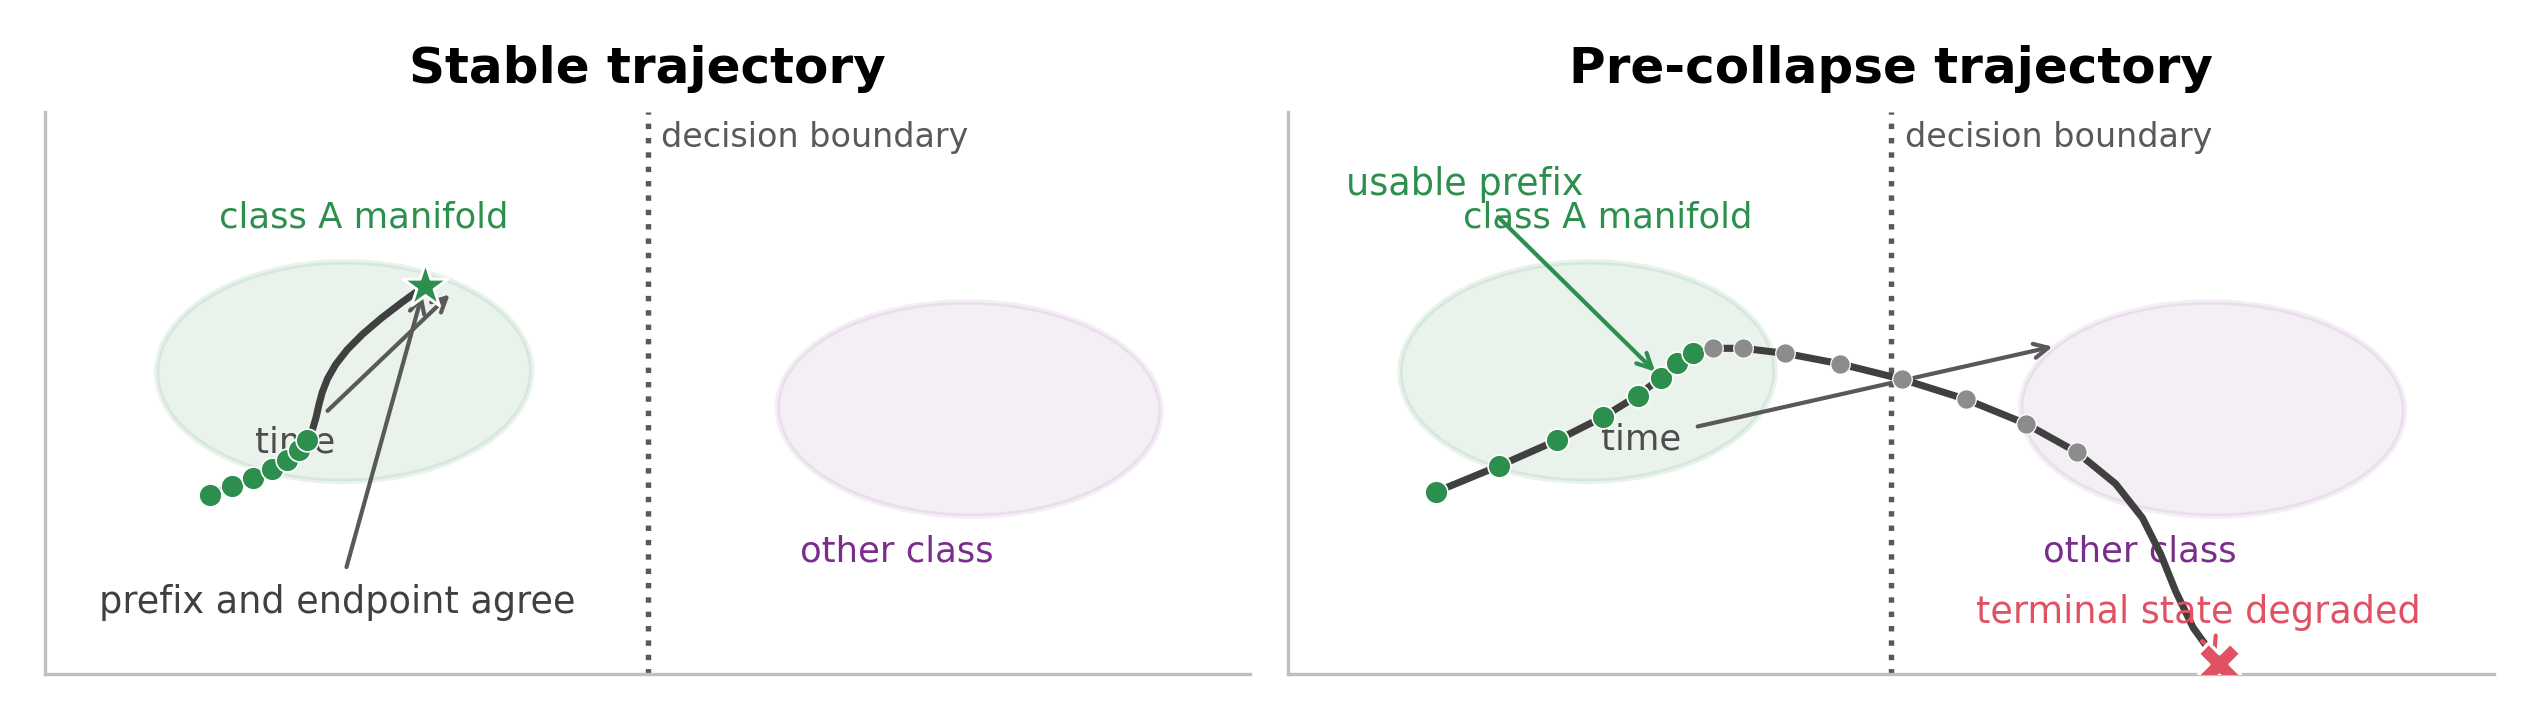
\includegraphics[width=0.90\linewidth]{fig0_precollapse_schematic}
  \vspace{-0.6em}
  \caption{\textbf{Conceptual picture of the pre-collapse regime.}
  In a stable trajectory, prefix states and the endpoint agree on the class
  label. In a pre-collapse trajectory, nonlinear amplification distorts the
  late state while predictive prefix states remain inside the correct class
  region. The failure is one of readout timing, not of the system's underlying
  computation.}
  \label{fig:precollapse_schematic}
  \vspace{-0.8em}
\end{figure}

Classical reservoir practice often sets the spectral radius $\rho(\bW)<1$ for
stability, but that prescription is neither always available nor sufficient.
In trained iterative systems, effective gain is learned; in physical and analog
in-memory substrates, variability, drift, input power, and nonlinearity change
rollout dynamics~\citep{leGallo2023mixed,wan2022compute,
rasch2024fast,momeni2025training}; and non-normal amplification can produce
large transient growth even when spectral radius suggests stability
~\citep{trefethen2005spectra,hennequin2012nonnormal,kerg2019nonnormal}.

\paragraph{Contributions.}
\begin{enumerate}
    \item We identify the \emph{pre-collapse learning regime} and formalise an
    accuracy-defined prefix grace period $G(\rho,\alpha)$: terminal-state
    inference fails before computational utility is lost, with empirically
    monotone shortening across the tested spectral sweep
    (\Cref{sec:discovery} and \Cref{sec:mechanism}).
    \item We characterise the regime across unbounded, bounded, and linear
    systems, and replicate the
    endpoint-vs.-trajectory mismatch on CIFAR-10 (with FashionMNIST in the appendix)
    (\Cref{sec:cross_system}).
    \item We show the regime persists in a trained LeakyReLU classifier even
    when trained at the unstable operating point: training postpones but does
    not suppress endpoint failure, with early-window recovering up to
    $+26.5$~pp; a trained row-sequential CIFAR-10 LSTM shows the same smaller
    bounded-gate pattern (\Cref{sec:trained_system,app:seq_cifar_lstm}).
    \item On Tiny ImageNet-200, recursive SwiGLU and shared-attention heads
    exhibit endpoint deterioration under inference-horizon extension, while
    matched-horizon training restores endpoint validity
    (\Cref{sec:tinyimagenet}).
    \item We distinguish the accuracy-defined prefix from a practical
    norm-ratio proxy and compare fixed early-window readout, adaptive
    stopping, and \grace{} as potential decoders, characterising their
    strengths and limitations across dynamical settings
    (\Cref{sec:exploit,sec:cross_system}).
\end{enumerate}

\paragraph{Scope and non-claims.}
We do not claim edge-of-chaos optimality, competitive CIFAR-10 performance,
universal dominance of \grace{} over simpler prefix readouts, or DEQ
convergence theory. Why not simply keep $\rho(\bW)<1$? We use spectral radius
as a controlled probe, not an operating recommendation; the broader issue is
endpoint validity under finite-time instability.

\paragraph{Relation to prior work.}
Transient recurrent dynamics can carry information beyond fixed-point
readout~\citep{maass2002real,jaeger2001echo}, and reservoir recipes already
use averaged or windowed states~\citep{lukosevicius2012practical}. Our
contribution is different in kind: a supercritical endpoint-validity failure
regime, operationalised through a prefix grace period, a norm-ratio proxy, and
a trained-system validation. Adaptive computation and test-time compute ask how
much inference compute to allocate~\citep{graves2016adaptive,
banino2021pondernet,snell2024testtime,geiping2025recurrent}; we ask whether
the terminal readout remains valid once that computation enters an unstable
regime. Early-exit and overthinking work studies depth-indexed intermediate
heads~\citep{teerapittayanon2016branchynet,kaya2019shallow,
elhoushi2024layerskip}; here the axis is time and the stop signal is the
trajectory norm ratio. Work on criticality, signal propagation, and non-normal
amplification explains when recurrent and deep systems preserve or amplify
information~\citep{bertschinger2004real,dambre2012information,
poole2016exponential,schoenholz2017deep,trefethen2005spectra,
hennequin2012nonnormal,kerg2019nonnormal}; we ask when endpoint-based
inference fails before that transient information is exhausted.

% =============================================================================
% 2. PROBLEM SETUP AND DEFINITIONS
% =============================================================================

\section{Background and Setup}
\label{sec:setup}

We make the endpoint convention precise and isolate the temporally asymmetric
failure of endpoint readout. Complex-valued and unitary dynamics~\citep{
trabelsi2018deep,arjovsky2016unitary} provide rich substrates; complex modReLU
makes the regime especially legible by preserving phase while permitting
magnitude growth.

In Sections~\ref{sec:discovery} through~\ref{sec:exploit} and the
fixed-substrate experiments of Section~\ref{sec:cross_system},
we study dynamical learners of the form
\begin{equation}
    \bz_{t+1} = \sigma(\bW \bz_t + \bU \bx + \mathbf{b}),
    \qquad \bz_0 = \mathbf{0},
    \label{eq:dynamics}
\end{equation}
where $\bx \in \R^n$ is a fixed input, $\bW \in \C^{d \times d}$ is the
recurrent weight matrix with spectral radius $\sr$, $\bU \in \C^{d \times n}$
is the input projection, $\mathbf{b}\in\C^d$ is a bias, and $\sigma$ is a
pointwise nonlinearity. The weights $\bW$, $\bU$, and $\mathbf{b}$ are fixed
(not trained), and learning occurs solely in a downstream linear probe. This
controlled setting isolates representational dynamics from training dynamics:
the regime, if present, is a property of rollout geometry rather than of
optimisation. Section~\ref{sec:trained_system} relaxes the fixed-substrate
assumption with a weight-tied iterative classifier whose recurrent weights,
input projection, bias, and head are jointly trained, testing whether the
regime survives when training shapes the terminal representation.

Rolling the system for a fixed horizon $T$ produces a trajectory
$(\bz_1, \ldots, \bz_T)$; in the main experiments, $T=40$. We compare four
readout strategies. The \textit{final-state} readout
$\phi_{\text{final}} = f(\bz_T)$ is the standard baseline. The
\textit{early-window} readout
$\phi_{\text{early}} = \frac{1}{K}\sum_{t=1}^{K} f(\bz_t)$ averages the
first $K \ll T$ steps.
The \textit{adaptive stopping} readout $\phi_{\text{stop}} = f(\bz_{\hat{t}})$
halts at the first timestep where the safeguarded norm ratio
$\|\bz_t\|/\max(\|\bz_1\|,\epsilon_{\mathrm{num}})$ exceeds a threshold
$\tau_{\text{stop}}$. Finally, \grace{}
(\emph{Growth-Regulated Adaptive State Extraction}) computes a per-sample
norm-ratio-weighted average over the full trajectory, down-weighting timesteps
whose norm ratio exceeds a threshold (\Cref{sec:grace}). Here
$f(\bz) = [\operatorname{Re}(\bz),
\operatorname{Im}(\bz)]$ maps complex states to real features; for real-valued
systems $f(\bz) = \bz$.

\begin{definition}[Prefix grace period]
\label{def:grace_period}
For a fixed dataset split, probe-training protocol, and dynamical system with
spectral radius $\sr$ and accuracy threshold $\alpha$, the \emph{grace period}
is the usable prefix length
\begin{equation}
    G(\sr, \alpha) =
    \max\!\left(\{0\}\cup\{T' \in \{1,\ldots,T\} :
    \operatorname{acc}(\phi_t) \geq \alpha
    \text{ for all } 1 \leq t \leq T'\}\right),
\end{equation}
where $\phi_t=f(\bz_t)$ is the single-timestep readout and
$\operatorname{acc}(\phi_t)$ is measured by training and evaluating a separate
linear probe using only features from timestep $t$. The definition is
intentionally prefix-based: if the first timestep fails, $G=0$; if accuracy
dips below $\alpha$ and later recovers, the grace period still ends at the
first failure. Thus $G$, $\operatorname{acc}(\cdot)$, and
$\operatorname{acc}_0$ below are empirical finite-sample quantities conditional
on the stated evaluation protocol.
\end{definition}

\begin{definition}[Pre-collapse learning regime]
\label{def:regime}
Fix margins $\Delta > 0$ and $0 < \epsilon < \Delta$. A dynamical system
with spectral radius $\sr$ operates in the \emph{pre-collapse learning regime}
when terminal accuracy has degraded from the stable baseline $\operatorname{acc}_0$,
$\operatorname{acc}(\phi_{\text{final}})<\operatorname{acc}_0-\Delta$, while a
usable prefix remains:
$G(\sr,\operatorname{acc}_0-\epsilon)>0$.
Here $\operatorname{acc}_0$ is measured by the same readout/probe protocol at a
stable reference configuration (in the main spectral sweep, $\rho(\bW)=0.5$;
for trained-system checks, the corresponding training operating point).
\end{definition}

We use $\Delta = 5$~pp and $\epsilon = 1$~pp throughout.

\begin{remark}
The pre-collapse regime is distinct from the edge-of-chaos
regime~\citep{bertschinger2004real}: it concerns systems operating
\emph{past} the critical boundary ($\sr > 1$), not at it, and it
characterises temporally asymmetric representational quality in the
supercritical phase rather than optimality at criticality.
\end{remark}

% =============================================================================
% 3. EMPIRICAL DISCOVERY
% =============================================================================

\section{Empirical Discovery of the Pre-Collapse Regime}
\label{sec:discovery}

We instantiate \Cref{eq:dynamics} on flattened MNIST~\citep{lecun1998gradient}
with a complex modReLU
reservoir ($d=128$, $T=40$, bias $b=-0.5$), sweeping $\sr=0.5$ to $1.6$
across 10 random seeds. $\bW$ is drawn from the complex Ginibre
ensemble~\citep{ginibre1965statistical} and rescaled to the target radius;
$\bU$ is complex Gaussian and column-normalised. A RidgeClassifier
probe~\citep{pedregosa2011scikit} is trained/evaluated on a 5k/5k split;
values are mean $\pm$ std. The early-window baseline uses $K=10$, with
sensitivity in Appendix~\ref{app:k_sensitivity}.

\Cref{fig:phase_diagram} visualises the regime in the complex modReLU sweep.
In this sweep, the accuracy-defined grace period $G(\sr, 0.70)$ shortens as
spectral radius increases, remaining at the full $T=40$ horizon through
$\sr \leq 1.20$, then falling to $38.4$ at $\sr = 1.30$, $31.1$ at
$\sr = 1.40$, $20.2$ at $\sr = 1.50$, and $15.2$ at $\sr = 1.60$
(Appendix~\ref{app:grace_period}). Separately, a norm-threshold stopping-time
proxy also shortens and provides an online indicator of usable prefix length.

\begin{figure}[t]
  \centering
  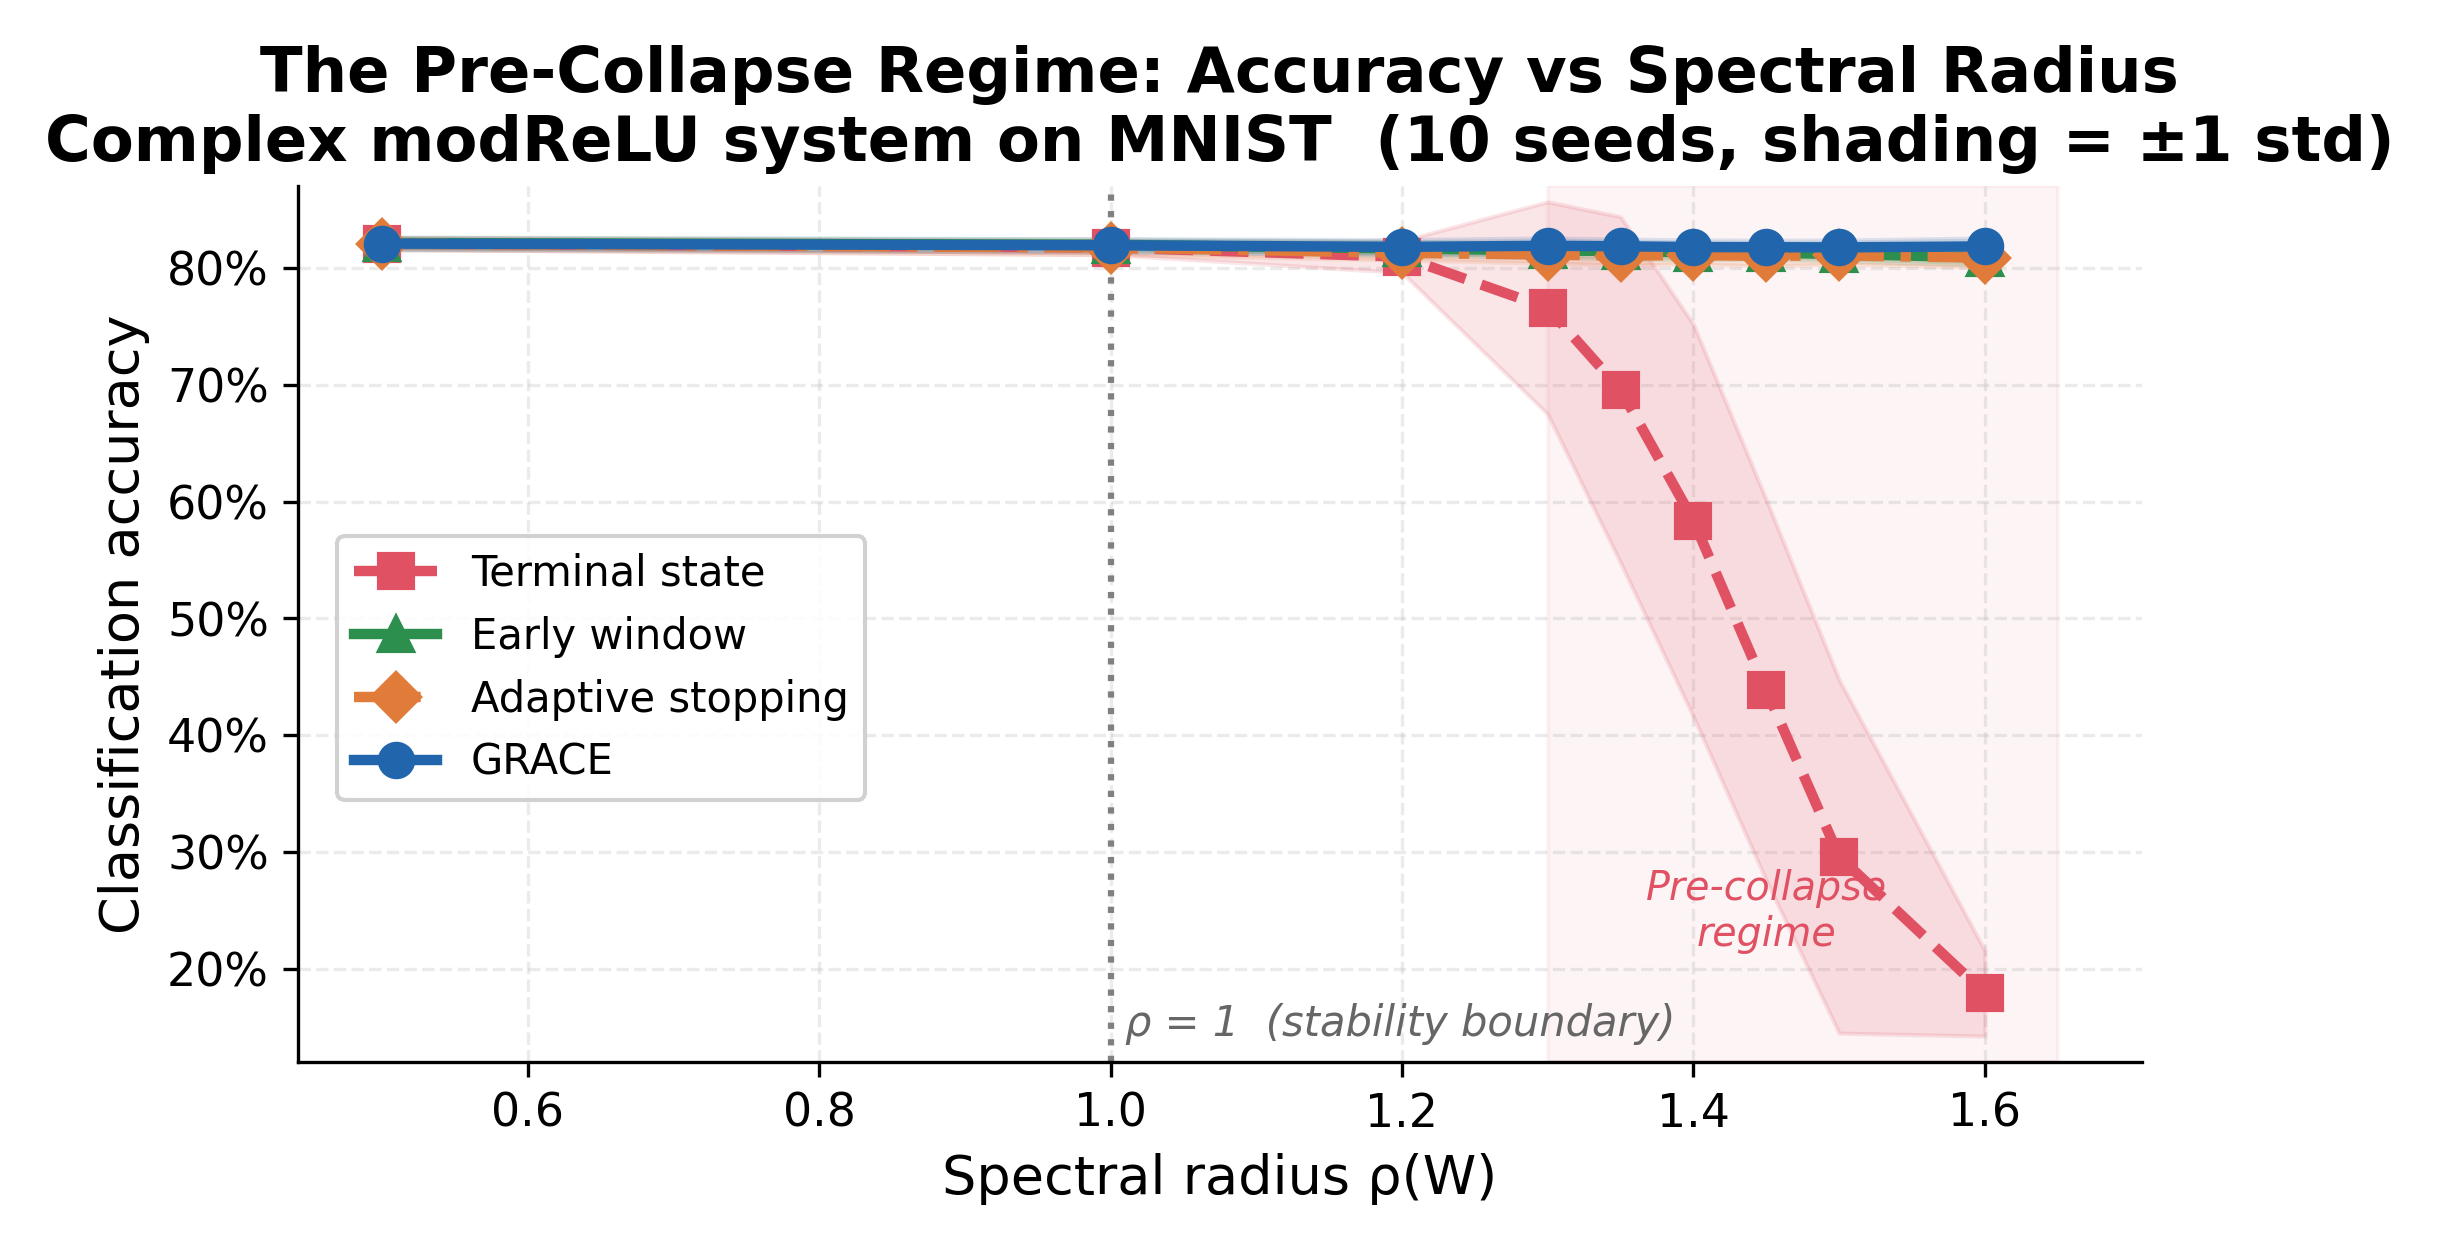
\includegraphics[width=0.80\linewidth]{fig1_phase_diagram}
  \caption{\textbf{The pre-collapse regime in the complex modReLU system.}
  As spectral radius increases, terminal-state accuracy collapses while
  early-window, adaptive stopping, and \grace{} remain near-flat (10 seeds;
  shading $=\pm1$ std). The pink region marks the pre-collapse band
  ($\rho \geq 1.30$) where endpoint-based evaluation fails. At $\rho=1.6$,
  \grace{} exceeds final-state readout by $64$~pp, and all cross-seed
  pair comparisons favour \grace{}.}
  \label{fig:phase_diagram}
\end{figure}

The quantitative summary in \Cref{tab:main} matches the visual transition in
\Cref{fig:phase_diagram}.
Terminal-state accuracy collapses from $82.1\%\pm 0.5$ at $\sr = 0.5$ to
$17.9\%\pm 3.7$ at $\sr = 1.6$, while non-terminal readouts remain near the
stable baseline; \grace{} reaches $81.9\%\pm 0.7$ at $\sr=1.6$.
Cohen's $d$ for \grace{} over final-state grows from $d = 0.30$ at
$\sr = 1.0$ to $d = 23.0$ at $\sr = 1.6$. This very large value should be
read together with the raw means and standard deviations: it reflects both
the $64$~pp mean separation and the fact that \grace{} sharply reduces
cross-seed standard deviation. A rank-based check gives Cliff's $\delta=1.0$ at
$\sr=1.6$ (all 100 cross-seed pairs favour \grace{} over final-state).

\begin{table}[t]
\centering
\caption{Readout accuracy (mean $\pm$ std, 10 seeds) across spectral radii
on MNIST. Non-terminal readouts maintain near-stable accuracy across the
unstable sweep. Cohen's $d$ is reported for \grace{} over final-state readout;
the largest values are driven by the combination of mean separation and
\grace{}'s reduced cross-seed standard deviation. At $\rho=1.6$, Cliff's
$\delta=1.0$.}
\label{tab:main}
\small
\begin{tabular}{l c c c c c}
\toprule
$\sr$ & Final & Early & Adaptive & \grace{} & Cohen's $d$\\
\midrule
0.50 & $0.821{\pm}0.005$ & $0.821{\pm}0.005$ & $0.821{\pm}0.005$ & $0.821{\pm}0.005$ & \phantom{0}$0.0$\\

1.00 & $0.818{\pm}0.006$ & $0.820{\pm}0.005$ & $0.818{\pm}0.006$ & $0.819{\pm}0.006$ & \phantom{0}$0.3$\\

1.20 & $0.810{\pm}0.014$ & $0.817{\pm}0.006$ & $0.813{\pm}0.006$ & $0.818{\pm}0.006$ & \phantom{0}$0.8$\\

1.30 & $0.766{\pm}0.091$ & $0.815{\pm}0.006$ & $0.811{\pm}0.007$ & $0.819{\pm}0.007$ & \phantom{0}$0.8$\\

1.35 & $0.696{\pm}0.148$ & $0.814{\pm}0.007$ & $0.811{\pm}0.008$ & $0.819{\pm}0.006$ & \phantom{0}$1.1$\\

1.40 & $0.584{\pm}0.168$ & $0.813{\pm}0.006$ & $0.811{\pm}0.008$ & $0.818{\pm}0.006$ & \phantom{0}$1.9$\\

1.45 & $0.439{\pm}0.163$ & $0.813{\pm}0.006$ & $0.810{\pm}0.009$ & $0.818{\pm}0.006$ & \phantom{0}$3.1$\\

1.50 & $0.296{\pm}0.151$ & $0.812{\pm}0.006$ & $0.811{\pm}0.008$ & $0.818{\pm}0.006$ & \phantom{0}$4.6$\\

1.60 & $0.179{\pm}0.037$ & $0.809{\pm}0.007$ & $0.809{\pm}0.008$ & $0.819{\pm}0.007$ & $23.0$\\

\bottomrule
\end{tabular}
\end{table}

We treat the coarse regime radii ($\sr \in \{1.3, 1.4, 1.5, 1.6\}$) as the
primary inferential family because each satisfies \Cref{def:regime} under
$\Delta = 5$~pp and $\epsilon = 1$~pp, and these are the main-text
operating points used for the headline claims. The intermediate radii
$1.35$ and $1.45$ are corroborating measurements included in the
appendix-wide audit. Across the primary family,
one-sided exact paired Wilcoxon signed-rank tests confirm that \grace{}
significantly outperforms final-state readout (all raw $p = 0.001$, the
minimum achievable for $n = 10$ non-tied paired samples under this one-sided
test) and early-window readout (raw $p \leq 0.007$ at all four radii), with
effect sizes ranging from
$d = 0.60$ to $d = 1.33$ for the \grace{}-vs-early comparison. After
Holm-Bonferroni correction across the eight primary tests (4~radii
$\times$ 2~comparisons), these remain significant. Broader sweeps across
all radii and auxiliary readout comparisons are reported as secondary
analyses in \Cref{app:stats}.

% =============================================================================
% 4. MECHANISM
% =============================================================================

\section{Mechanism: Why Terminal Failure Precedes Transient Failure}
\label{sec:mechanism}

The pre-collapse regime can be understood through a separation between two timescales:
the timescale at which discriminative structure is imprinted by the input
projection, and the timescale at which nonlinear amplification destroys it.
We formalise this below.

Consider two inputs $\bx, \bx'$ from distinct classes, producing trajectories
$\bz_t, \bz_t'$ under \Cref{eq:dynamics}. Define inter-class separation
$\delta_t = \|\bz_t - \bz_t'\|$. Since both trajectories start from
$\bz_0=\bz'_0=\mathbf{0}$, at $t = 1$,
\[
  \delta_1 =
  \|\sigma(\bU\bx + \mathbf{b}) - \sigma(\bU\bx' + \mathbf{b})\|,
\]
and the pre-activation difference is $\bU(\bx-\bx')$. Thus the initial class
separation is set by the input projection rather than the recurrent gain.
For later timesteps, the local Jacobian dynamics along each input-conditioned
trajectory are governed by the effective Jacobians
\[
  J_t = D\sigma(\bW \bz_t + \bU \bx + \mathbf{b})\,\bW.
\]
For complex modReLU, $D\sigma$ denotes the real Jacobian acting on stacked
$(\operatorname{Re} z,\operatorname{Im} z)$ coordinates, not a holomorphic
complex derivative.
In supercritical regimes, products of these Jacobians can amplify perturbations
sufficiently that late-time distortion overtakes the input-imprinted class
structure. This creates the observed temporal asymmetry: early timesteps are
dominated by useful input-driven separation, while later timesteps become
increasingly governed by recurrent amplification and nonlinear distortion.
The linearisation is local; for the smooth tanh branch,
\Cref{app:kreiss_refinement} makes the finite-separation claim precise by
comparing accumulated nonlinear remainder along the Jacobian cocycle with the
linear probe margin.

In a linear system ($\sigma = \text{id}$),
$\bz_{t+1} = \bW \bz_t + \bU \bx + \mathbf{b}$, trajectory differences remain
linear images of the input difference. Recurrent growth can rescale or rotate
features, but it cannot introduce activation-dependent gating or saturation
that progressively erodes class-discriminative structure. Empirically, our
linear null experiment exhibits no meaningful grace period: early and terminal
readouts remain nearly identical across the spectral sweep, indicating that in
the tested systems nonlinear distortion, rather than radial growth alone,
drives the regime. The pre-collapse regime therefore requires more than
spectral growth alone in our taxonomy; it appears with nonlinear state
distortion.

Nonlinear activations introduce the critical asymmetry. modReLU is
phase-preserving but magnitude-gated, zeroing components when $|z| + b \leq 0$;
with $b=-0.5$, this means $|z|\leq0.5$. This is relatively benign early, while
input projection dominates and the gated features remain separable, but under
supercritical recurrence the changing gating pattern compounds over time and
can erode class separability (Appendix~\ref{app:mechanism_diag}). The same
appendix shows that finite-time
operator amplification tracks grace-period shortening and terminal failure.
Bounded activations like tanh introduce a milder version: saturation compresses
large activations toward $\pm1$, reducing inter-class variance gradually.


\begin{proposition}[Grace-period upper bound]
\label{prop:grace}
Let $\bar r_t$ be a deterministic reference norm-ratio curve, such as the
dataset mean of
$\|\bz_t^{(i)}\|/\max(\|\bz_1^{(i)}\|,\epsilon_{\mathrm{num}})$, with
$\epsilon_{\mathrm{num}}>0$. Fix $\alpha \in (0,1)$.
Assume there exist $t_0 \in \{1,\ldots,T\}$ and $\kappa > 1$ such that
\[
  \bar r_t \geq \bar r_{t_0}\,\kappa^{t-t_0}
  \qquad \text{for all } t \geq t_0.
\]
Assume also that there exists $R_{\max} > 1$ with
$0<\bar r_{t_0}\leq R_{\max}$ such that
$\operatorname{acc}(\phi_t) < \alpha$ whenever $\bar r_t > R_{\max}$.
Then
\begin{equation}
    G(\sr,\alpha) \leq t_0 + \left\lceil
    \frac{\log(R_{\max} / \bar r_{t_0})}{\log \kappa}
    \right\rceil.
    \label{eq:grace_bound}
\end{equation}
\end{proposition}

The proof is in Appendix~\ref{app:proofs}.

\begin{remark}
Proposition~\ref{prop:grace} is a conditional growth argument, not a spectral
theorem. It says that once accuracy fails beyond a norm threshold and the
reference norm-ratio curve grows at least geometrically after $t_0$, the prefix
grace period is bounded. The proposition is deliberately stated at the
dataset-aggregate level, matching the aggregate probe accuracy in
\Cref{def:grace_period}, rather than as a per-sample stopping theorem. We do
not identify $\kappa$ with $\rho(\bW)$ in the non-normal
setting; empirically, larger $\rho$ coincides with faster norm-ratio growth and
shorter measured $G(\rho,\alpha)$ under post-$t_0=5$ fits
(\Cref{app:grace_period}). For smooth
activations, \Cref{app:kreiss_refinement} replaces $\kappa$ with a linearised
amplification envelope and the terminal cutoff with a margin-vs.-remainder
criterion.
\end{remark}

% =============================================================================
% 5. EXPLOITING THE REGIME
% =============================================================================

\section{Regime-Aware Decoding}
\label{sec:exploit}

The pre-collapse regime does not prescribe one decoder: fixed early-window
tests whether any usable prefix remains after terminal collapse, while adaptive
stopping and \grace{} add norm-ratio timing when the usable-prefix boundary is
sample-dependent or noisy.
Computationally, adaptive stopping can reduce inference cost by halting before
the full horizon. \grace{} still evaluates the trajectory to length $T$, but it
can be streamed with memory $O(\dim f(\bz))$ per sample, constant in $T$, by accumulating
$\sum_t \tilde w_t^{(i)}f(\bz_t^{(i)})$ and $\sum_t \tilde w_t^{(i)}$, rather
than storing all states.

\subsection{Adaptive Stopping}

A stopping rule based on the norm ratio provides a simple, effective baseline:
\begin{equation}
    \mathcal{T}_{\text{stop}}^{(i)} =
    \left\{t \in \{1,\ldots,T\} :
    \frac{\|\bz_t^{(i)}\|}
    {\max(\|\bz_1^{(i)}\|,\epsilon_{\mathrm{num}})}
    > \tau_{\text{stop}}\right\}
    \cup \{T\}, \qquad
    \hat{t}^{(i)} = \min \mathcal{T}_{\text{stop}}^{(i)}.
    \label{eq:stopping}
\end{equation}
Here the superscript $(i)$ indexes samples,
$\mathcal{T}_{\text{stop}}^{(i)}$ is the set of threshold-crossing timesteps
with fallback $T$, $\hat t^{(i)}$ is the selected stopping timestep,
$\tau_{\text{stop}}$ is the hard stopping threshold, and
$\epsilon_{\mathrm{num}}=10^{-10}$ keeps the ratio defined if the first-step
norm vanishes. We keep the rule minimal, with no learning or auxiliary state,
to isolate feature quality from the stopping policy. We fix
$\tau_{\text{stop}} = 1.5$ for the main experiments;
Appendix~\ref{app:selection_protocol} audits nearby thresholds and a
reference-radius selection at $\rho=1.3$.
The rule maintains ${\sim}81\%$ accuracy across $\sr = 0.5$ to $1.6$
(\Cref{fig:grace_method}), recovering $+63$~pp over terminal readout at
$\sr = 1.60$. If the threshold is never crossed, it defaults to $T$.

\subsection{\grace{}: Soft Norm-Weighted Trajectory Readout}
\label{sec:grace}

Rather than selecting a single stopping time, \grace{} computes a smooth
weighting over the entire trajectory:
\begin{align}
    g_t^{(i)} &= \frac{\|\bz_t^{(i)}\|}{\max(\|\bz_1^{(i)}\|,\epsilon_{\mathrm{num}})},
    \label{eq:growth} \\
    \tilde{w}_t^{(i)} &= \exp\bigl(-\alpha \max(0,\, g_t^{(i)} - \tau)\bigr),
    \label{eq:raw_weight} \\
    w_t^{(i)} &= \frac{\tilde{w}_t^{(i)}}{\sum_{s=1}^{T} \tilde{w}_s^{(i)}},
    \label{eq:normalize} \\
    \phi_{\grace{}}^{(i)} &= \sum_{t=1}^{T} w_t^{(i)}\, f(\bz_t^{(i)}),
    \label{eq:grace}
\end{align}
where $g_t^{(i)}$ is the per-sample norm ratio at timestep $t$,
$\tilde{w}_t^{(i)}$ is the unnormalised growth-penalised weight,
$w_t^{(i)}$ is its normalised version, $\tau$ is a threshold parameter,
and $\alpha\geq0$ controls penalty sharpness.

The interpretation is simple. In stable regimes, where $g_t \lesssim 1$
throughout the rollout, all unnormalised weights equal one and \grace{}
reduces to the transient mean. In unstable regimes, timesteps whose norm
ratio exceeds $\tau$ are exponentially down-weighted, so weight shifts
toward the usable prefix. Crucially, this weighting is per-sample rather
than global: different inputs can receive different temporal profiles.

The following proposition formalises the non-interference property:

\begin{proposition}[Threshold non-interference]
\label{prop:noninterfering}
For any trajectory $(\bz_1, \ldots, \bz_T)$, if
the safeguarded ratios $g_t \leq \tau$ for all $t = 1, \ldots, T$,
then \grace{} assigns uniform weights $w_t = 1/T$ for all $t$, and
therefore reduces exactly to transient-mean readout.
\end{proposition}

\begin{proof}
If $g_t \leq \tau$, then $\max(0, g_t - \tau) = 0$, so each unnormalised
weight equals $\exp(0) = 1$. Normalisation yields $w_t = 1/T$.
\end{proof}

In the stable regime of our experiments ($\sr \leq 1.0$), the observed norm
ratios remain close to unity, so \grace{} behaves nearly identically to
uniform trajectory averaging there.

\Cref{fig:grace_method} makes this behaviour visible. The
x-axis is timestep and curve colour indicates spectral radius. At $\sr = 1.0$,
weights are close to uniform; at $\sr = 1.3$, they are front-loaded but still
broad; at $\sr = 1.5$, the first timestep receives about one third of the total
weight and the first ten receive roughly $55\%$. Thus \grace{} does not estimate
the grace period and then read uniformly across it; the norm ratio constructs a
conservative per-sample schedule inside the usable prefix. The profile is also a
regime diagnostic, shifting from full-trajectory averaging toward prefix
extraction as the substrate enters the pre-collapse band, consistent with the
reduction in cross-seed variability in \Cref{app:variance}.


\begin{figure}[H]
  \centering
  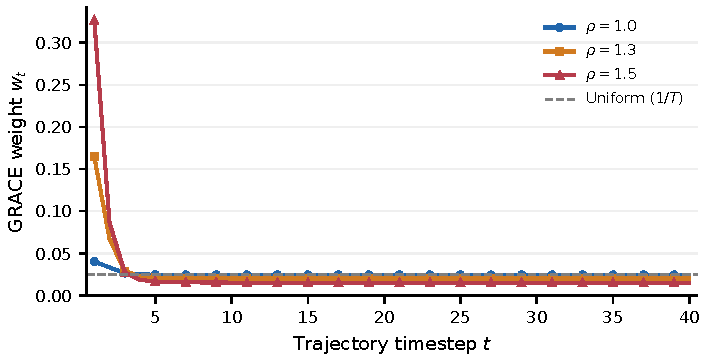
\includegraphics[width=0.73\linewidth]{fig3_grace_method.pdf}
  \caption{\textbf{\grace{} as a soft regime-aware prefix selector.}
  Temporal weight profiles for three spectral radii; curve
  colour indicates $\rho$ and the x-axis is trajectory timestep. Weights shift
  from near-uniform ($\rho=1.0$) to front-loaded ($1.3$) to
  prefix-concentrated ($1.5$;
  $\tau=1.2,\alpha=10$).}
  \label{fig:grace_method}
\end{figure}

In the fixed complex-modReLU sweep, this soft prefix selection is useful. With
$\tau = 1.2$ and $\alpha = 10$, \grace{} stays in the $81.8$--$82.1\%$ range
across the full spectral sweep, while terminal-state readout falls to
$17.9\%$. Its gain over early-window is modest but consistent, growing from
$+0.4$~pp at $\sr = 1.30$ to $+1.0$~pp at $\sr = 1.60$.

The more important benefit in this setting is stability. In the transition
band ($\sr = 1.40$), the standard deviation of terminal-state accuracy reaches
$0.168$, while \grace{} reduces this to $0.006$, a $27\times$ reduction
(\Cref{app:variance}). In the same fixed complex-modReLU reservoir under
injected dynamical noise, \grace{} also remains stable while adaptive stopping degrades by $3$--$4$~pp at
$\sr \in \{1.4, 1.5\}$ (\Cref{app:noise}).

% =============================================================================
% 6. CROSS-SYSTEM AND CROSS-DATASET EVIDENCE
% =============================================================================

\section{Generality Across Systems, Datasets, and Training Regimes}
\label{sec:cross_system}

To assess generality, we replicate the core experiments across complex modReLU
(unbounded), real-valued tanh ESN (bounded), and linear dynamics
($\sigma=\text{id}$), with additional curves in \Cref{app:cross_system}. At
$\sr=1.6$, the endpoint-vs.-trajectory gap is large in complex modReLU,
moderate in the real ESN, and essentially zero in the linear null.
\Cref{fig:cifar10,fig:cifar10_resnet18_main,fig:trained_system} show the same
question on CIFAR-10 and trained iterative systems.

The decoder taxonomy is nonlinearity-dependent. In complex modReLU dynamics,
\grace{} is strongest at $\sr=1.6$ ($+0.7$~pp over both early-window and
adaptive stopping). In bounded tanh ESNs, adaptive stopping and the best
\grace{} configuration are essentially tied ($84.5\%$ vs.\ $84.3\%$). In
linear systems, the gap is negligible ($+0.002$), confirming that spectral
instability alone does not create a grace period.

\subsection{Harder-Benchmark Generality: CIFAR-10}
\label{sec:cifar10}

To test whether the regime is an artefact of simple class structure, we repeat
the complex modReLU experiment on CIFAR-10~\citep{krizhevsky2009learning}
($d{=}512$, $T{=}40$, 10 seeds, 5k/5k split). On raw pixels, terminal readout
falls to $10.6\%$ at $\sr=1.6$ while \grace{} holds at
$34.2\pm0.7\%$ ($+23.7$~pp). On frozen ImageNet ResNet-18
features~\citep{he2016deep}, a direct ridge probe reaches $85.2\%\pm0.1$; at
$\sr=1.6$, terminal readout falls to $26.2\%\pm2.3$ while early-window and
\grace{} remain at $84.5\%\pm0.1$ and $84.0\%\pm0.1$. Thus the gap survives
translation to an $85\%$-accuracy substrate. FashionMNIST and frozen-feature
details are in \Cref{app:fashion,app:cifar_resnet18}.



\begin{figure}[H]
  \centering
  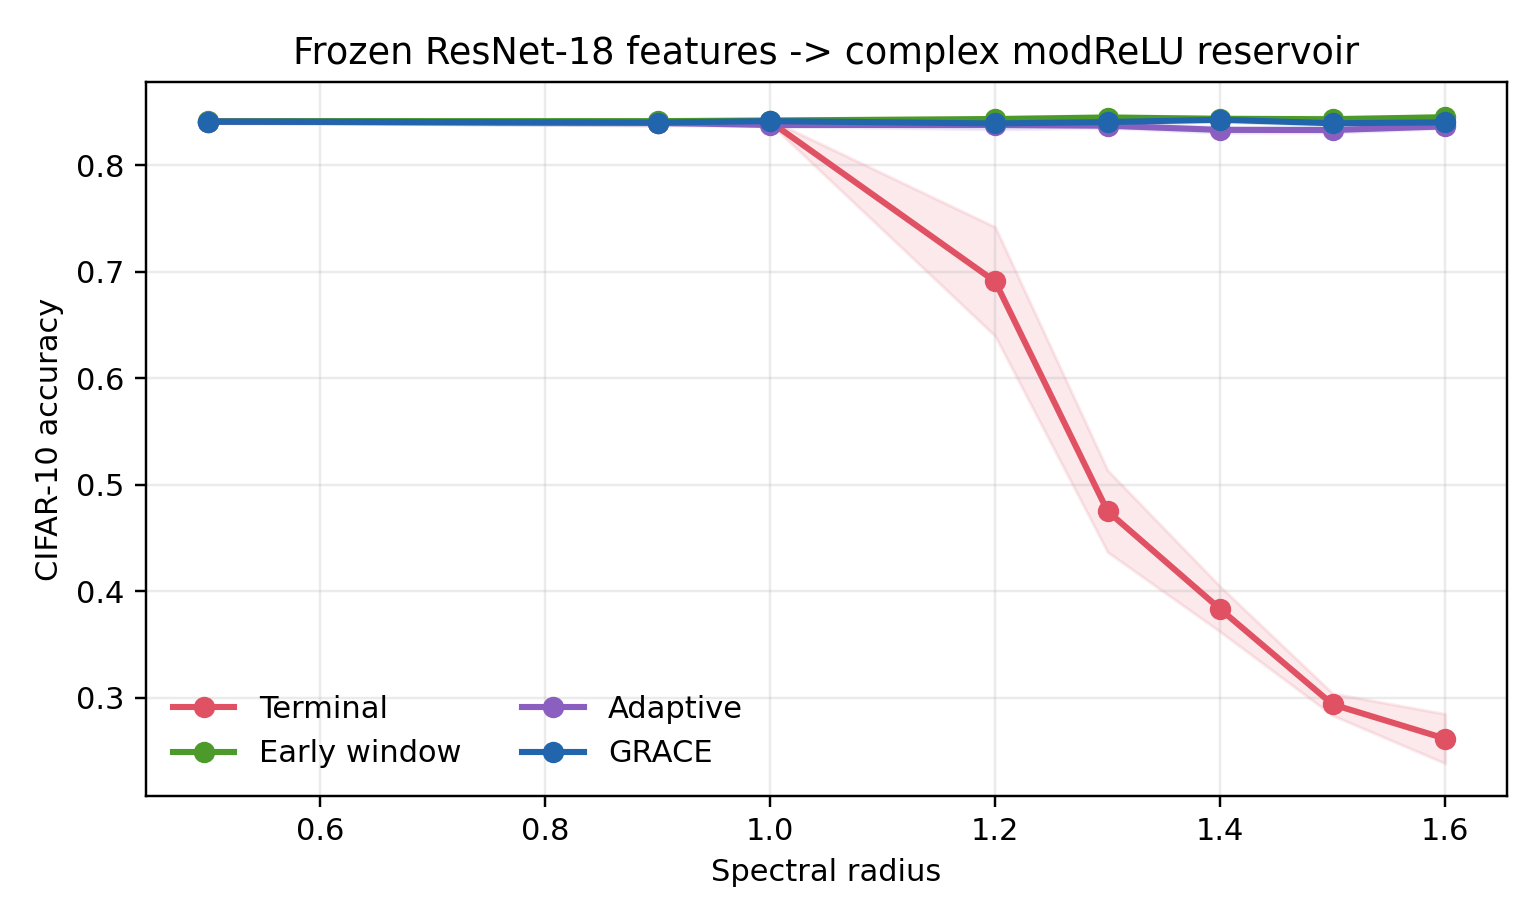
\includegraphics[width=0.74\linewidth]{fig_cifar10_resnet18_regime}
  \caption{\textbf{Pre-collapse regime on CIFAR-10 with frozen ResNet-18
  features.} A direct ridge probe on ImageNet-pretrained ResNet-18 features
  reaches $85.2\%\pm0.1$ accuracy. Passing those 512-dimensional features
  through the same complex modReLU reservoir preserves the
  endpoint-vs.-trajectory gap: at $\sr=1.6$, terminal readout falls to $26.2\%\pm2.3$,
  while early-window and \grace{} remain near $84\%$ (5 seeds; shading
  $=\pm1$ std).}
  \label{fig:cifar10_resnet18_main}
\end{figure}

\subsection{Trained Iterative Systems}
\label{sec:trained_system}

A natural objection is that fixed reservoirs make endpoint failure too easy, so
we test whether the mismatch survives when terminal representations are shaped
by optimisation. Our first trained check is a weight-tied LeakyReLU iterative
classifier on flattened MNIST, with recurrence
\begin{equation}
    \bz_{t+1} = \text{LeakyReLU}\bigl(\lambda \bW \bz_t + \bU \bx + \mathbf{b}\bigr),
    \qquad \bz_0 = \mathbf{0},
    \label{eq:trained_dynamics}
\end{equation}
where $\bW \in \R^{256 \times 256}$, $\bU \in \R^{256 \times 784}$, and the
recurrent weights, input projection, bias, and linear head are jointly trained
from terminal-state cross-entropy. Across 5 seeds, we compare
$T_{\text{train}}=10,\lambda_{\text{train}}=0.85$ with two at-operating-point
conditions ($T_{\text{train}}=40$, $\lambda_{\text{train}}\in\{1.20,1.30\}$);
all reach ${\geq}96\%$ training accuracy. Details are in \Cref{app:details}.

\Cref{fig:trained_system} summarises the main results; full statistics are in
\Cref{app:trained_table}. In A, final accuracy drops from $92.0\%$ to $79.4\%$
by $\lambda=2.0$, while early-window remains near $95.2\%$ ($+15.8$~pp). In
B1/B2, terminal readout is locally optimal near the training gain but collapses
to $69.4\%$ and $77.3\%$ at $\lambda=2.0$, while early-window remains
$95.9\%$ ($+26.5$ and $+18.6$~pp). Training delays but does not suppress the
regime. A standard row-sequential CIFAR-10 LSTM shows the same smaller
bounded-gate pattern: early-window is $+3.5$~pp over terminal at $\lambda=2.0$,
and a single-timestep probe audit gives accuracy-defined prefix lengths
$40,27,2$ at $\lambda\in\{1.0,1.6,2.0\}$ (\Cref{app:seq_cifar_lstm}).

\begin{figure}[t]
  \centering
  \makebox[\linewidth][c]{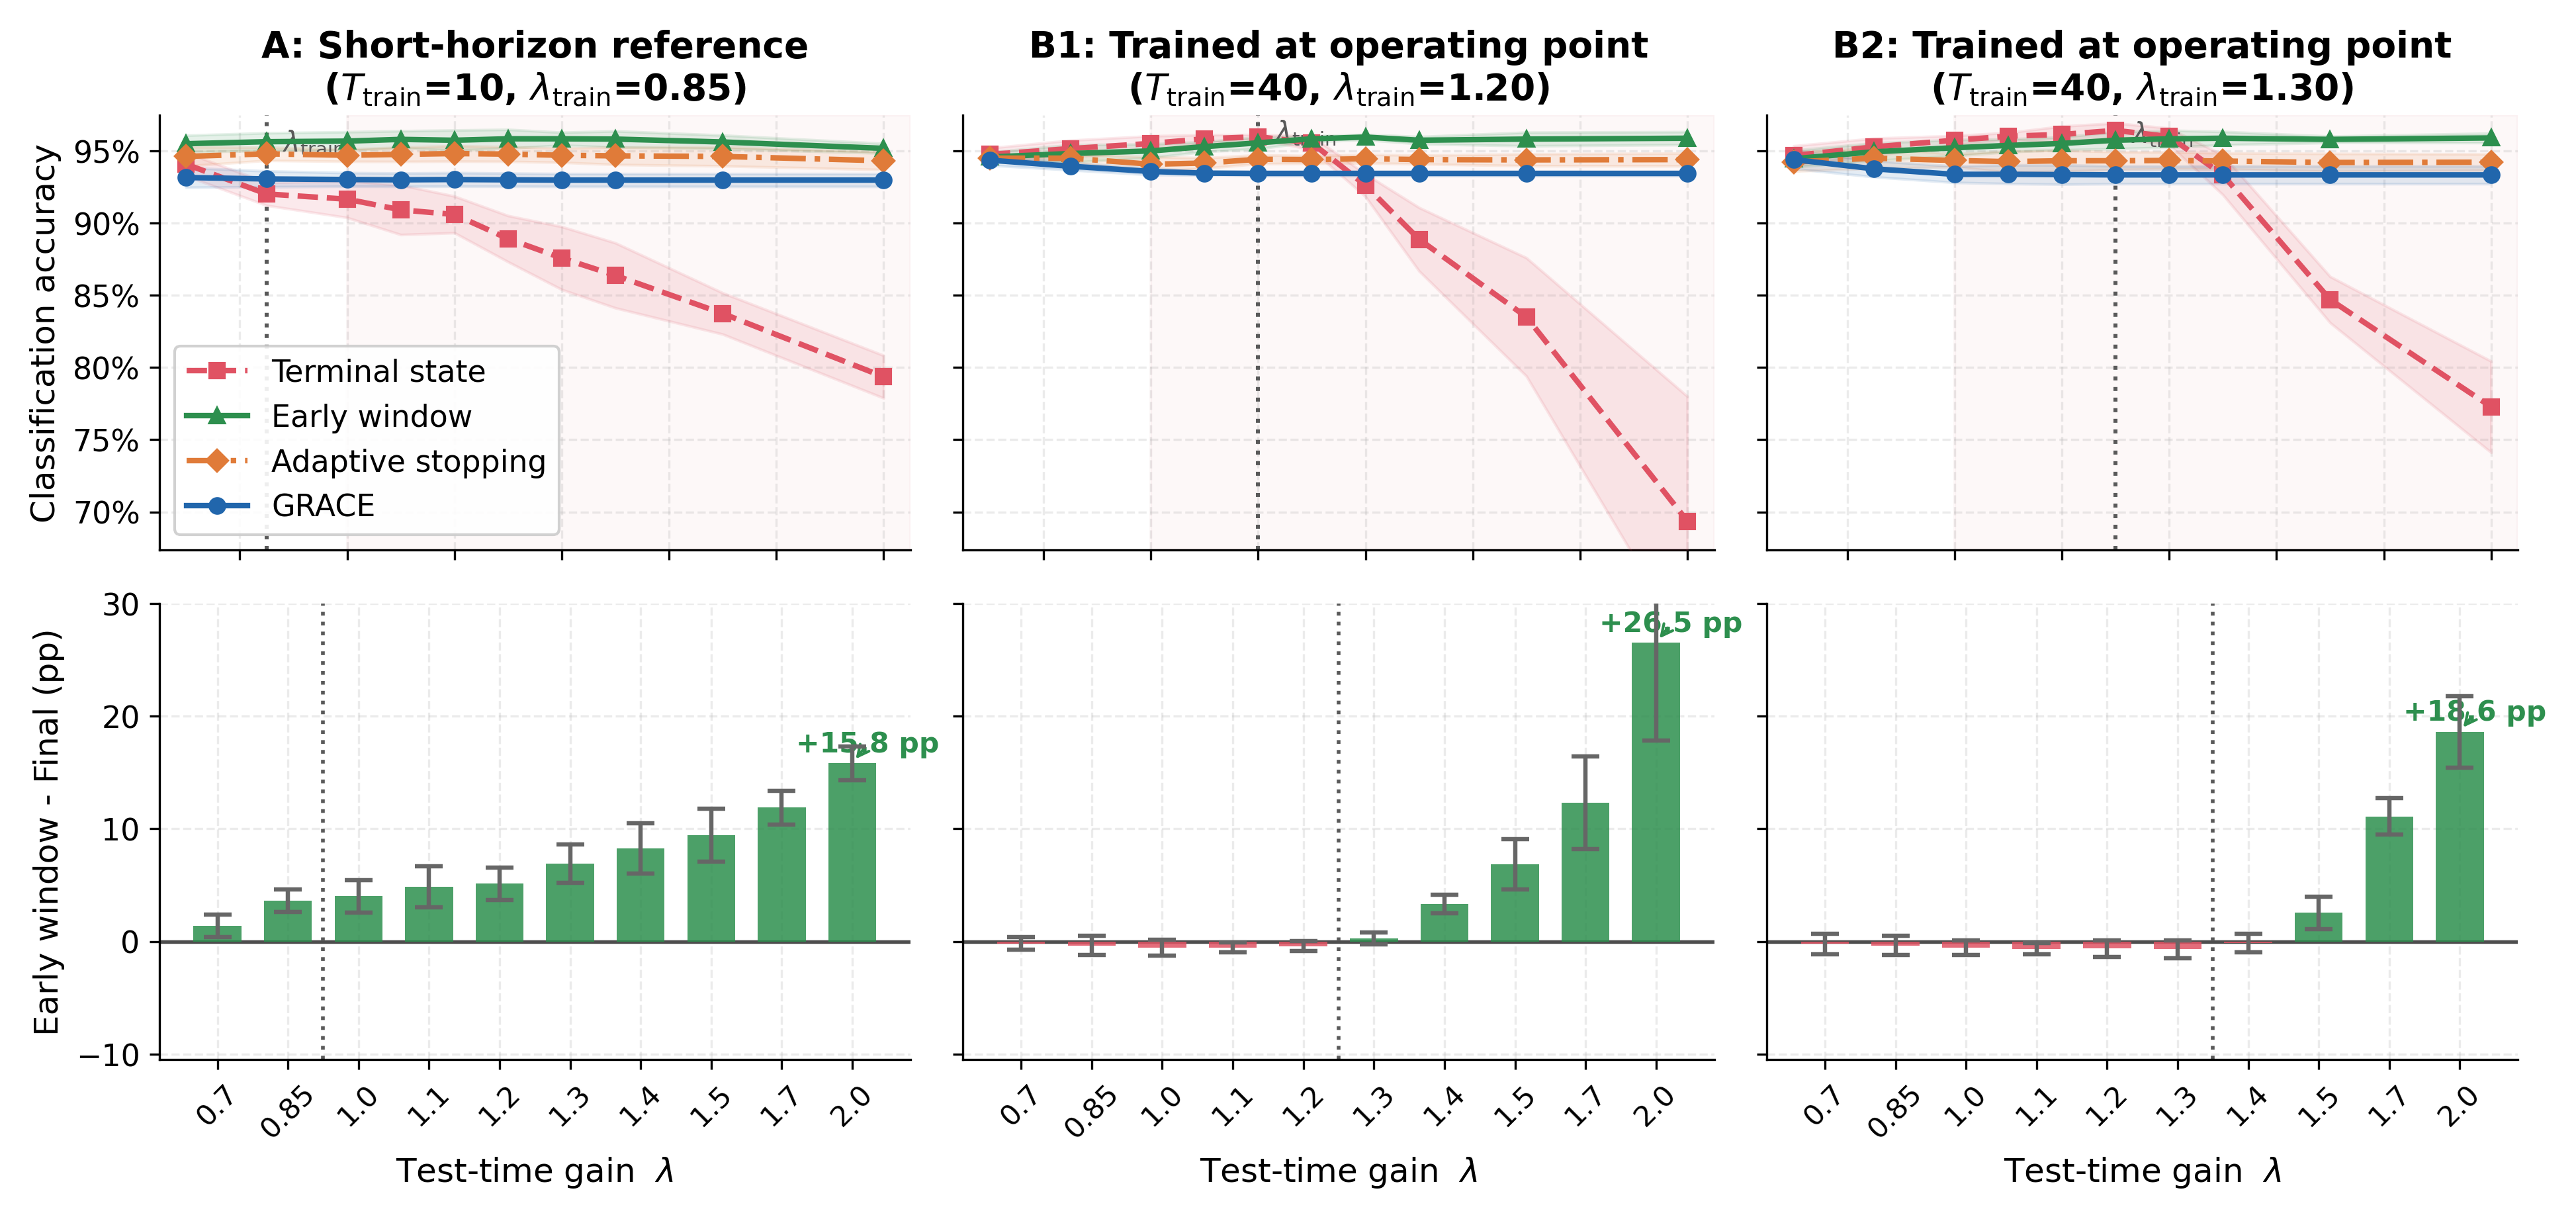
\includegraphics[width=0.92\linewidth]{fig6_trained_system}}
  \caption{\textbf{Training at the operating point postpones but does not suppress
  the pre-collapse regime.} Columns are training conditions; top row shows
  accuracy vs.\ test-time gain $\lambda$, and bottom row shows early-window
  minus terminal accuracy. Peak gains are $+15.8$, $+26.5$, and $+18.6$~pp.}
  \label{fig:trained_system}
\end{figure}

% =============================================================================
% 7. DISCUSSION
% =============================================================================

\FloatBarrier
\subsection{Modern Recursive Models on Tiny ImageNet}
\label{sec:tinyimagenet}

We test horizon extension on Tiny ImageNet-200 (100k training/10k labelled
validation images), using frozen ConvNeXt-Tiny features~\citep{liu2022convnext}
and weight-tied SwiGLU and shared-attention heads. Both use terminal
cross-entropy, $T_{\rm train}\in\{8,32\}$, and paired seeds 101--103.
Evaluation uses $T_{\rm test}\in\{8,16,24,32\}$ at gain 1, with residual
scale $1/T_{\rm train}$ fixed. Matched controls change training depth and
scale together; architecture details are in \Cref{app:modern_protocol}.

\begin{figure}[!htbp]
  \centering
  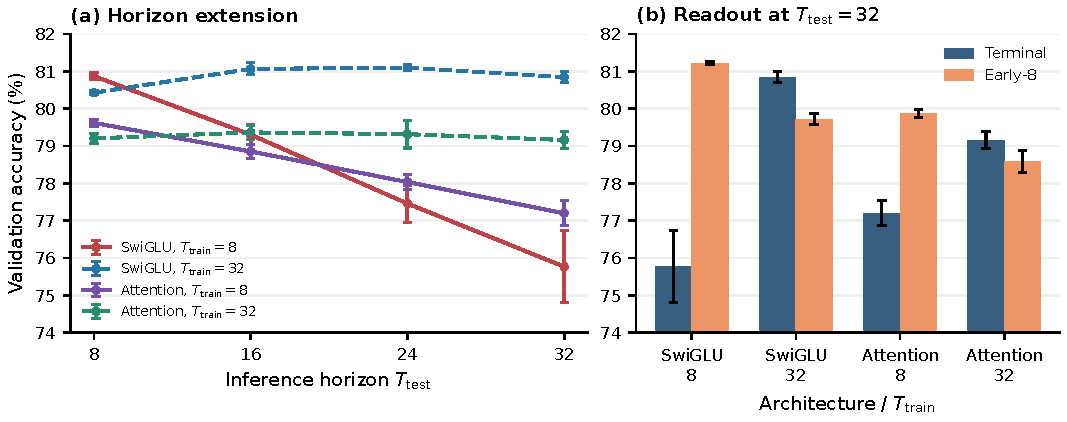
\includegraphics[width=\linewidth]{fig_modern_horizon_readout.pdf}
  \caption{\textbf{Horizon extension and early-prefix readout on Tiny ImageNet.}
  \emph{(a)} Terminal accuracy over inference horizons for eight- and
  32-step-trained SwiGLU and attention heads. \emph{(b)} Terminal versus
  early-eight readout at $T_{\rm test}=32$. Early readout preserves accuracy
  under horizon mismatch, while matched training restores a competitive
  endpoint. Means and sample standard deviations across three paired seeds;
  frozen ConvNeXt-Tiny backbone.}
  \label{fig:modern_panel}
\end{figure}

In \Cref{fig:modern_panel}, extending the eight-step-trained SwiGLU
model to 32 steps lowers terminal accuracy from $80.87\pm0.09\%$ to
$75.76\pm0.96\%$, a $5.11\pm0.94$~pp loss; early-eight readout retains
$81.22\pm0.05\%$. Shared attention reproduces the pattern: terminal accuracy
falls from $79.62\pm0.10\%$ to $77.20\pm0.34\%$ ($2.42\pm0.29$~pp), while
early-eight readout remains at $79.88\pm0.11\%$. Fixed-regularisation probes
also lose $2.23\pm0.17$ and $1.28\pm0.08$~pp, respectively, indicating
reduced linear decodability beyond shared-head mismatch.

Matched 32-step training removes the strong endpoint loss: SwiGLU reaches
$80.84\pm0.15\%$ at step 32, and attention loses only $0.04\pm0.17$~pp from
steps 8 to 32. The paired difference in terminal loss between training
conditions is $5.53\pm0.92$~pp for SwiGLU and $2.38\pm0.43$~pp for attention,
positive in every seed; all states and logits remain finite. These statistics
are descriptive, without significance claims (complete readouts and robustness
analyses in \Cref{app:modern_readouts,app:modern_robustness}).

The SwiGLU effect depends on checkpoint age: retained final-epoch checkpoints
lose only $0.59$--$0.68$~pp, compared with $4.27$--$6.13$~pp at the selected
checkpoints. Attention degradation persists across its retained checkpoint
audit (\Cref{app:modern_robustness}).

\subsection{Inference Time and Memory}
\label{sec:cost}

We benchmark six readouts on a separate seed-0 SwiGLU model with cached
ConvNeXt features (\Cref{tab:cost_main}). Early-eight readout takes $1.80$~ms
versus terminal's $6.73$~ms by executing fewer steps. Streaming \grace{}
reduces additional peak allocation from $48.56$ to $8.51$~MiB but is slower;
adaptive stopping incurs active-set overhead. Lower storage does not guarantee
lower latency. \Cref{app:modern_cost} details the protocol and complexity.

\begin{table}[H]
\centering
\caption{\textbf{Measured recurrent-head inference cost.} RTX 5080 Laptop GPU,
BF16, batch 512, $d=512$, $T=32$, gain 1.3; median of 25 repetitions after
10 warm-ups. Memory is additional peak allocated memory above the warmed-up
baseline. Image decoding and backbone inference are excluded.}
\label{tab:cost_main}
\small
\begin{tabular}{lrr}
\toprule
Readout & Latency (ms) & Additional peak (MiB) \\
\midrule
Terminal & 6.727 & 8.00 \\
Early window ($K=8$) & 1.803 & 11.50 \\
Adaptive stopping & 13.840 & 9.01 \\
Uniform streaming & 6.889 & 8.50 \\
\grace{}, stored trajectory & 6.948 & 48.56 \\
\grace{}, streaming & 9.681 & 8.51 \\
\bottomrule
\end{tabular}
\end{table}


\section{Discussion}
\label{sec:discussion}

Decoder effectiveness depends on the dynamics: early windows are strongest in
the trained LeakyReLU and LSTM checks, while \grace{} is useful under unbounded
growth and injected noise (\Cref{app:noise}). Matched training restores modern
recursive endpoints. Early readout is therefore a diagnostic and possible
remedy, with benefits conditional on the dynamics and training horizon.

Physical substrates face similar timing questions because device variability,
temperature, and wear can shift operating points~\citep{leGallo2023mixed,
wan2022compute,rasch2024fast}. Norm ratios are measurable without knowing
$\rho(\bW)$~\citep{tanaka2019recent,momeni2025training,wanjura2025fully,
wang2024large}. Practically, early readout saves recurrent steps, whereas
streaming \grace{} saves storage without guaranteeing lower latency
(\Cref{sec:cost}).

Related questions arise in continuous-depth graph models~\citep{poli2019graph}, a natural setting for
studying readout validity over integration time. Graph diffusion connects
depth to smoothing of node features~\citep{chamberlain2021grand}, suggesting
the analogous question of whether intermediate states retain task information
lost at the endpoint. Diffusive homogenisation differs from the
amplification-driven distortion studied here; neither our norm-growth proxy
nor our nonlinear taxonomy transfers automatically. Trajectory readouts for
graph ODEs remain an open empirical direction.

Limitations include controlled gain and horizon shifts, frozen vision
backbones, and three seeds per modern condition. Tiny ImageNet validation also
selects checkpoints. These laptop-GPU experiments establish conditional
endpoint failure. Assessing its prevalence in large deployed models remains
future work, alongside extensions to graph ODEs and state-space models and
tighter bounds.

% =============================================================================
% 8. CONCLUSION
% =============================================================================

\section{Conclusion}

Usable prefixes can persist after terminal collapse. Gain-shift experiments
and horizon-extension tests in modern recursive heads expose endpoint-validity
failures; matched training restores endpoint validity in the latter setting.
Readout timing and the training horizon are therefore part of the algorithm.

\clearpage
\bibliographystyle{plainnat}
% \bibliography{references}

\begin{thebibliography}{46}

\bibitem{jaeger2001echo}
H.~Jaeger.
\newblock The ``echo state'' approach to analysing and training recurrent neural
  networks.
\newblock Technical Report GMD Report 148, German National Research Center for
  Information Technology, 2001.

\bibitem{bai2019deep}
S.~Bai, J.~Z. Kolter, and V.~Koltun.
\newblock Deep equilibrium models.
\newblock In \emph{NeurIPS}, 2019.

\bibitem{chen2018neural}
R.~T.~Q. Chen, Y.~Rubanova, J.~Bettencourt, and D.~Duvenaud.
\newblock Neural ordinary differential equations.
\newblock In \emph{NeurIPS}, 2018.

\bibitem{he2016deep}
K.~He, X.~Zhang, S.~Ren, and J.~Sun.
\newblock Deep residual learning for image recognition.
\newblock In \emph{CVPR}, 2016.

\bibitem{trabelsi2018deep}
C.~Trabelsi, O.~Bilaniuk, Y.~Zhang, D.~Serdyuk, S.~Subramanian, J.~F. Santos,
  S.~Mehri, N.~Rostamzadeh, Y.~Bengio, and C.~J. Pal.
\newblock Deep complex networks.
\newblock In \emph{ICLR}, 2018.

\bibitem{arjovsky2016unitary}
M.~Arjovsky, A.~Shah, and Y.~Bengio.
\newblock Unitary evolution recurrent neural networks.
\newblock In \emph{ICML}, 2016.

\bibitem{ginibre1965statistical}
J.~Ginibre.
\newblock Statistical ensembles of complex, quaternion, and real matrices.
\newblock \emph{Journal of Mathematical Physics}, 6(3):440--449, 1965.

\bibitem{tao2010random}
T.~Tao, V.~Vu, and M.~Krishnapur.
\newblock Random matrices: Universality of {ESDs} and the circular law.
\newblock \emph{Annals of Probability}, 38(5):2023--2065, 2010.

\bibitem{lukosevicius2012practical}
M.~Luko{\v{s}}evi{\v{c}}ius.
\newblock A practical guide to applying echo state networks.
\newblock In \emph{Neural Networks: Tricks of the Trade}, pages 659--686.
  Springer, 2012.

\bibitem{graves2016adaptive}
A.~Graves.
\newblock Adaptive computation time for recurrent neural networks.
\newblock \emph{arXiv preprint arXiv:1603.08983}, 2016.

\bibitem{banino2021pondernet}
A.~Banino, J.~Balaguer, and C.~Blundell.
\newblock {PonderNet}: Learning to ponder.
\newblock \emph{arXiv preprint arXiv:2107.05407}, 2021.

\bibitem{cohen2021gradient}
J.~M. Cohen, S.~Kaur, Y.~Li, J.~Z. Kolter, and A.~Talwalkar.
\newblock Gradient descent on neural networks typically occurs at the edge of
  stability.
\newblock In \emph{ICLR}, 2021.

\bibitem{bertschinger2004real}
N.~Bertschinger and T.~Natschl{\"a}ger.
\newblock Real-time computation at the edge of chaos in recurrent neural
  networks.
\newblock \emph{Neural Computation}, 16(7):1413--1436, 2004.

\bibitem{dambre2012information}
J.~Dambre, D.~Verstraeten, B.~Schrauwen, and S.~Massar.
\newblock Information processing capacity of dynamical systems.
\newblock \emph{Scientific Reports}, 2:514, 2012.

\bibitem{poole2016exponential}
B.~Poole, S.~Lahiri, M.~Raghu, J.~Sohl-Dickstein, and S.~Ganguli.
\newblock Exponential expressivity in deep neural networks through transient
  chaos.
\newblock In \emph{NeurIPS}, 2016.

\bibitem{schoenholz2017deep}
S.~S. Schoenholz, J.~Gilmer, S.~Ganguli, and J.~Sohl-Dickstein.
\newblock Deep information propagation.
\newblock In \emph{ICLR}, 2017.

\bibitem{yildiz2012revisiting}
I.~B. Yildiz, H.~Jaeger, and S.~J. Kiebel.
\newblock Re-visiting the echo state property.
\newblock \emph{Neural Networks}, 35:1--9, 2012.

\bibitem{trefethen2005spectra}
L.~N. Trefethen and M.~Embree.
\newblock \emph{Spectra and Pseudospectra: The Behavior of Nonnormal Matrices
  and Operators}.
\newblock Princeton University Press, 2005.

\bibitem{pascanu2013difficulty}
R.~Pascanu, T.~Mikolov, and Y.~Bengio.
\newblock On the difficulty of training recurrent neural networks.
\newblock In \emph{ICML}, pages 1310--1318, 2013.

\bibitem{bengio1994learning}
Y.~Bengio, P.~Simard, and P.~Frasconi.
\newblock Learning long-term dependencies with gradient descent is difficult.
\newblock \emph{IEEE Transactions on Neural Networks}, 5(2):157--166, 1994.

\bibitem{maass2002real}
W.~Maass, T.~Natschl{\"a}ger, and H.~Markram.
\newblock Real-time computing without stable states: A new framework for
  neural computation based on perturbations.
\newblock \emph{Neural Computation}, 14(11):2531--2560, 2002.

\bibitem{tanaka2019recent}
G.~Tanaka, T.~Yamane, J.~B. H{\'e}roux, R.~Nakane, N.~Kanazawa, S.~Takeda,
  H.~Numata, D.~Nakano, and A.~Hirose.
\newblock Recent advances in physical reservoir computing: A review.
\newblock \emph{Neural Networks}, 115:100--123, 2019.

\bibitem{leGallo2023mixed}
M.~Le Gallo, R.~Khaddam-Aljameh, M.~Stanisavljevic, et~al.
\newblock A 64-core mixed-signal in-memory compute chip based on phase-change
  memory for deep neural network inference.
\newblock \emph{Nature Electronics}, 6:680--693, 2023.

\bibitem{wan2022compute}
W.~Wan, R.~Kubendran, C.~Schaefer, et~al.
\newblock A compute-in-memory chip based on resistive random-access memory.
\newblock \emph{Nature}, 608:504--512, 2022.

\bibitem{rasch2024fast}
M.~J. Rasch, F.~Carta, O.~Fagbohungbe, et~al.
\newblock Fast and robust analog in-memory deep neural network training.
\newblock \emph{Nature Communications}, 15:7133, 2024.

\bibitem{momeni2025training}
A.~Momeni, B.~Rahmani, B.~Scellier, et~al.
\newblock Training of physical neural networks.
\newblock \emph{Nature}, 645:53--61, 2025.

\bibitem{wanjura2025fully}
C.~C. Wanjura and F.~Marquardt.
\newblock Fully non-linear neuromorphic computing with linear wave scattering.
\newblock In \emph{Proceedings of SPIE}, volume 13375, page 133750H, 2025.

\bibitem{wang2024large}
H.~Wang, J.~Hu, A.~Morandi, et~al.
\newblock Large-scale photonic computing with nonlinear disordered media.
\newblock \emph{Nature Computational Science}, 4:429--439, 2024.

\bibitem{gallicchio2017echo}
C.~Gallicchio and A.~Micheli.
\newblock Echo state property of deep reservoir computing networks.
\newblock \emph{Cognitive Computation}, 9(3):337--350, 2017.

\bibitem{hennequin2012nonnormal}
G.~Hennequin, T.~P. Vogels, and W.~Gerstner.
\newblock Non-normal amplification in random balanced neuronal networks.
\newblock \emph{Physical Review E}, 86(1):011909, 2012.


\bibitem{teerapittayanon2016branchynet}
S.~Teerapittayanon, B.~McDanel, and H.~T.~Kung.
\newblock Branchynet: Fast inference via early exiting from deep neural
  networks.
\newblock In \emph{ICPR}, 2016.

\bibitem{kaya2019shallow}
Y.~Kaya, S.~Hong, and T.~Dumitras.
\newblock Shallow-deep networks: Understanding and mitigating network
  overthinking.
\newblock In \emph{ICML}, 2019.

\bibitem{kerg2019nonnormal}
G.~Kerg, K.~Goyette, M.~Puelma Touzel, G.~Gidel, E.~Vorontsov, Y.~Bengio, and
  G.~Lajoie.
\newblock Non-normal recurrent neural network (nnRNN): learning long time
  dependencies while improving expressivity with transient dynamics.
\newblock In \emph{NeurIPS}, 2019.

\bibitem{snell2024testtime}
C.~Snell, J.~Lee, K.~Xu, and A.~Kumar.
\newblock Scaling {LLM} test-time compute optimally can be more effective than
  scaling parameters for reasoning.
\newblock In \emph{ICLR}, 2025.

\bibitem{geiping2025recurrent}
J.~Geiping, S.~M. McLeish, N.~Jain, J.~Kirchenbauer, S.~Singh,
  B.~R. Bartoldson, B.~Kailkhura, A.~Bhatele, and T.~Goldstein.
\newblock Scaling up test-time compute with latent reasoning: A recurrent depth
  approach.
\newblock In \emph{NeurIPS}, spotlight, 2025.

\bibitem{elhoushi2024layerskip}
M.~Elhoushi, A.~Shrivastava, D.~Liskovich, B.~Hosmer, B.~Wasti,
  L.~Lai, A.~Mahmoud, B.~Acun, S.~Agarwal, A.~Roman, A.~Aly,
  B.~Chen, and C.-J. Wu.
\newblock {LayerSkip}: Enabling early exit inference and self-speculative
  decoding.
\newblock In \emph{ACL}, 2024.

\bibitem{gabor2024pcdeq}
M.~Gabor, T.~Piotrowski, and R.~L.~G. Cavalcante.
\newblock Positive concave deep equilibrium models.
\newblock In \emph{ICML}, 2024.

\bibitem{lin2026consistency}
J.~Lin, Z.~Ling, J.~Xu, and R.~C. Qiu.
\newblock Consistency deep equilibrium models.
\newblock \emph{arXiv preprint arXiv:2602.03024}, 2026.

\bibitem{lecun1998gradient}
Y.~LeCun, L.~Bottou, Y.~Bengio, and P.~Haffner.
\newblock Gradient-based learning applied to document recognition.
\newblock \emph{Proceedings of the IEEE}, 86(11):2278--2324, 1998.

\bibitem{xiao2017fashion}
H.~Xiao, K.~Rasul, and R.~Vollgraf.
\newblock Fashion-{MNIST}: A novel image dataset for benchmarking machine
  learning algorithms.
\newblock \emph{arXiv preprint arXiv:1708.07747}, 2017.

\bibitem{krizhevsky2009learning}
A.~Krizhevsky.
\newblock Learning multiple layers of features from tiny images.
\newblock Technical report, University of Toronto, 2009.

\bibitem{pedregosa2011scikit}
F.~Pedregosa, G.~Varoquaux, A.~Gramfort, V.~Michel, B.~Thirion, O.~Grisel,
  M.~Blondel, P.~Prettenhofer, R.~Weiss, V.~Dubourg, J.~VanderPlas,
  A.~Passos, D.~Cournapeau, M.~Brucher, M.~Perrot, and {\'E}.~Duchesnay.
\newblock Scikit-learn: Machine learning in {Python}.
\newblock \emph{Journal of Machine Learning Research}, 12:2825--2830, 2011.

\bibitem{liu2022convnext}
Z.~Liu, H.~Mao, C.-Y. Wu, C.~Feichtenhofer, T.~Darrell, and S.~Xie.
\newblock A ConvNet for the 2020s.
\newblock In \emph{CVPR}, 2022.

\bibitem{poli2019graph}
M.~Poli, S.~Massaroli, J.~Park, A.~Yamashita, H.~Asama, and J.~Park.
\newblock Graph neural ordinary differential equations.
\newblock \emph{arXiv preprint arXiv:1911.07532}, 2019.

\bibitem{chamberlain2021grand}
B.~Chamberlain, J.~Rowbottom, M.~I. Gorinova, M.~Bronstein, S.~Webb, and E.~Rossi.
\newblock {GRAND}: Graph neural diffusion.
\newblock In \emph{ICML}, pages 1407--1418, 2021.

\end{thebibliography}

% =============================================================================
% APPENDIX
% =============================================================================

\appendix

\section{Additional Experimental Details}
\label{app:details}

\paragraph{System parameters.}
All complex modReLU experiments use $d = 128$, $n = 784$, modReLU bias
$b = -0.5$, rollout $T = 40$, magnitude clipping at $|\bz| > 50$, and no
injected noise ($\sigma_{\text{noise}} = 0$) unless otherwise stated. The
clipping threshold is a
numerical safeguard; our claim is that non-terminal readouts retain
separability before terminal degradation, not that clipping is the mechanism
of terminal collapse. The input projection $\bU$
is drawn i.i.d.\ complex Gaussian and normalised. The recurrent weight
$\bW$ is drawn from the complex Ginibre ensemble and rescaled to the target
spectral radius. Real ESN uses the same architecture with $\sigma = \tanh$,
unit leak rate, and real-valued weights of matching dimension.
MNIST, FashionMNIST, and the cross-system sweep use $d=128$ reservoirs. These
are robustness checks rather than exhaustive capacity studies; the real-ESN
comparison is a qualitative decoder-taxonomy check rather than a matched
real-valued capacity benchmark.

A dedicated clipping audit on the same 10 seeds and 5k held-out MNIST samples
confirms that the usable early prefix is not created by the hard threshold:
no state entry is clipped in the first 10 timesteps at any spectral radius.
Across the full 40-step rollout, the mean clipped-entry fraction is
$0.25\%$ at $\rho=1.40$, $1.33\%$ at $\rho=1.50$, and $4.06\%$ at
$\rho=1.60$; the earliest clipping event across all runs occurs at
$t=12$. Thus the late terminal state can encounter the numerical
safeguard at the largest radii, but the early-window evidence and the
prefix selected by \grace{} lie before clipping is active.

The stronger CIFAR-10 feature experiment in \Cref{app:cifar_resnet18} uses
frozen ImageNet-pretrained ResNet-18 penultimate features (512 dimensions),
a stratified 10k subset of the CIFAR-10 training split, and the full 10k
test split. The downstream complex modReLU reservoir uses $d=512$, $T=40$,
5 seeds, and exact eigenvalue spectral-radius rescaling.

\Cref{fig:ginibre_spectrum} visualises the random-matrix substrate used in
the complex modReLU sweep. The unscaled complex Ginibre ensemble has the
standard circular-law spectral geometry in high dimension
\citep{ginibre1965statistical,tao2010random}, and our experimental sweep
rescales this cloud radially to the requested spectral radius. This diagnostic
is only a substrate check: the pre-collapse regime does not follow from the
circular law alone, but from radial scaling interacting with finite-time
amplification, input imprinting, and nonlinear modReLU distortion.

\begin{figure}[H]
  \centering
  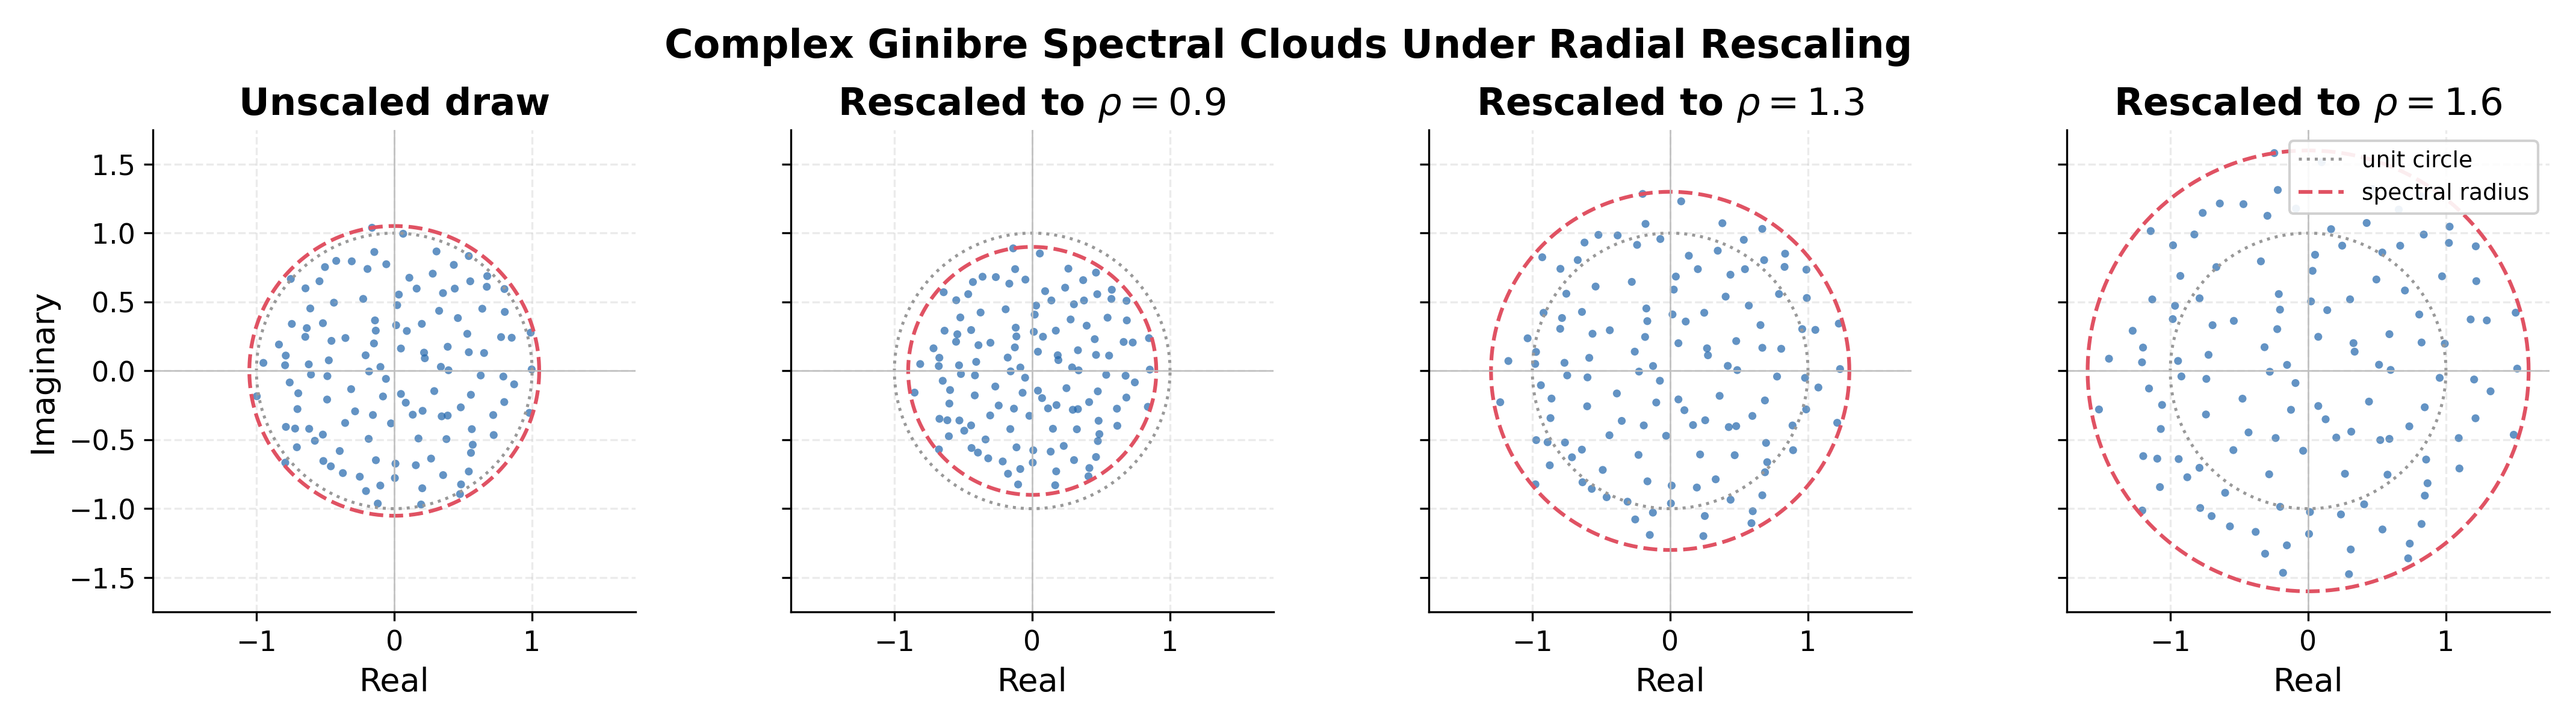
\includegraphics[width=0.88\linewidth]{fig12_ginibre_spectrum}
  \caption{\textbf{Complex Ginibre spectral clouds before and after
  spectral-radius rescaling.} Each panel shows one $d=128$ complex Ginibre
  draw rescaled to the target spectral radius. The figure documents the
  canonical circular-law substrate used in the spectral sweep; it is not a
  mechanism claim for the pre-collapse regime by itself.}
  \label{fig:ginibre_spectrum}
\end{figure}

\paragraph{Probe.}
All aggregate readout results use \texttt{RidgeClassifierCV} from scikit-learn with
leave-one-out cross-validation for the regularisation parameter
\citep{pedregosa2011scikit}. This
provides a closed-form solution with no iterative optimisation, ensuring
that all accuracy differences reflect the quality of the dynamical features
rather than probe optimisation artefacts. The dense single-timestep LSTM audit
in \Cref{app:seq_cifar_lstm} uses fixed ridge regularisation
$\alpha_{\rm ridge}=1.0$ for computational tractability.

\paragraph{Trained iterative systems.}
The LeakyReLU trained-system experiments use flattened MNIST with 10k training
examples and 2k test examples. The model has hidden dimension 256, LeakyReLU
negative slope 0.2, and state clipping to $[-100,100]$. It is trained
end-to-end from terminal-state cross-entropy with Adam (learning rate
$10^{-3}$, weight decay $10^{-4}$), cosine annealing, batch size 256, and
gradient-norm clipping (1.0 in condition A, 0.5 in B1/B2). Condition A trains
for 40 epochs at $T_{\text{train}}=10,\lambda_{\text{train}}=0.85$; conditions
B1/B2 train for 60 epochs at $T_{\text{train}}=40$ with
$\lambda_{\text{train}}\in\{1.20,1.30\}$. Evaluation uses
$T_{\text{test}}=40$ over
$\lambda_{\text{test}}\in\{0.7,0.85,1.0,1.1,1.2,1.3,1.4,1.5,1.7,2.0\}$
and 5 random seeds. After training, readout accuracies are measured with the
same RidgeClassifierCV protocol on extracted readout features, fitting on the
first 1k held-out test examples and scoring on the remaining 1k; this keeps
final, early-window, adaptive, and \grace{} readouts under a common probe.

The row-sequential CIFAR-10 LSTM check in \Cref{app:seq_cifar_lstm} uses 10k/2k
CIFAR-10, a 512-hidden-unit LSTM trained end-to-end with AdamW for 30 epochs,
and readouts from a 40-step zero-input post-image settling trajectory; the
appendix gives the full training and timestep-audit protocol.

\paragraph{Readout hyperparameters.}
All reservoir experiments use early-window $K=10$; trained-system
experiments use $K=8$. Adaptive stopping uses the fixed default
$\tau_{\text{stop}} = 1.5$ in the main paper.

\paragraph{Datasets and usage terms.}
MNIST is used via torchvision's standard benchmark distribution derived from
the original NIST release~\citep{lecun1998gradient}. FashionMNIST is
distributed by Zalando under the MIT License~\citep{xiao2017fashion}.
CIFAR-10 is used from the Alex Krizhevsky / University of Toronto benchmark
distribution, which requests citation of the original technical
report~\citep{krizhevsky2009learning}. The raw-pixel, frozen-feature, and
row-sequential LSTM CIFAR-10 checks all use standard train/test splits; the
frozen-feature CIFAR-10 check uses torchvision's ImageNet-pretrained ResNet-18
weights as a fixed feature extractor.

\paragraph{\grace{} hyperparameters.}
The primary configuration uses $\tau = 1.2$, $\alpha = 10$. An anchor
configuration ($\tau = 1.5$, $\alpha = 5$) is reported for robustness.
Appendix~\ref{app:selection_protocol} gives a lightweight reference-radius
audit at $\rho = 1.3$: it selects a slightly more aggressive frozen
alternative, but the qualitative conclusions and method ordering remain
unchanged.

\paragraph{Compute resources.}
The original reservoir, CIFAR-10, and trained LeakyReLU/LSTM experiments
were run on a single local CUDA-capable GPU
(NVIDIA RTX PRO 1000 Blackwell Generation Laptop GPU, 8~GB VRAM). The
core 10-seed MNIST reservoir sweep took $10{,}737$~s ($\approx 3.0$~h),
the dynamical-noise study $2{,}720$~s ($\approx 45$~min), the
accuracy-defined grace-period appendix analysis $360$~s ($\approx 6$~min),
and the readout-audit appendix sweep $13{,}952$~s ($\approx 3.9$~h), as
recorded in the saved result files. Additional reported experiments
(FashionMNIST, CIFAR-10, trained LeakyReLU, cross-system sweeps, the DEQ
relevance check, and the sequential CIFAR-10 LSTM check) were run on the same
single-GPU setup; the LSTM check and per-timestep audit were hour-scale runs
(the saved audit run recorded $3{,}229$~s for 3 seeds). The compute for these original experiments
remains comfortably below one day of GPU time overall. Pilot and
discarded exploratory runs required additional compute of comparable order,
but not orders of magnitude more than the reported totals.
The frozen ResNet-18 CIFAR-10 feature extraction took approximately 3~min
including the one-time ImageNet-weight download, and the cached 5-seed
spectral sweep took $243$~s ($\approx4.1$~min).
The small compute footprint is useful for reproducibility, but it is also a
limitation: the present experiments are stress tests of the readout regime,
not evidence that the same quantitative gaps will persist unchanged in much
larger, production-scale models.

The additional Tiny ImageNet experiments used an RTX 5080 Laptop GPU;
their configurations, runtime, and memory measurements are reported in
\Cref{app:modern_protocol,app:modern_cost}.

\section{Trained-System Readout Statistics}
\label{app:trained_table}

\Cref{tab:e6} gives full per-condition readout accuracy for the trained
LeakyReLU classifier across all three training conditions and selected
test-time gains. Bold entries mark the gain at which final-state
readout is locally optimal (i.e.\ at or just above the training gain).
Training uses flattened MNIST (10k/2k), hidden dimension 256, terminal-state
cross-entropy, Adam with learning rate $10^{-3}$ and weight decay $10^{-4}$,
cosine annealing, batch size 256, 40 epochs for condition A and 60 for
B1/B2, and the condition-specific $T_{\text{train}}$ and
$\lambda_{\text{train}}$ values listed in the table. The full gain sweep is
$\lambda_{\text{test}}\in\{0.7,0.85,1.0,1.1,1.2,1.3,1.4,1.5,1.7,2.0\}$;
as in the script, reported readout accuracies use RidgeClassifierCV probes fit
on the first half of the 2k held-out subset and scored on the second half.

To verify that the \grace{} underperformance is structural rather than a
tuning artefact, we swept $\tau \in \{0.5, 0.8, 1.0, 1.2, 1.5, 2.0,
3.0\}$ and $\alpha \in \{2, 5, 10, 20, 50\}$ using the per-timestep probe
accuracies and norm trajectories stored from the trained-system runs. The best
configuration ($\tau=3.0$, $\alpha=2$, which approaches uniform weighting)
recovers approximately $1.0$~pp over the default ($\tau=1.2$, $\alpha=10$)
but remains $1.0$--$2.0$~pp below early-window in conditions A and B1, and
is essentially tied in condition B2 near the training gain.
The gap therefore does not close under re-tuning. The mechanistic reason is
that the norm ratio in the trained system is a less informative readout-timing
signal: the early trajectory contains a representation-building phase in
which norms increase without implying discriminability loss, while the
learned head has absorbed expected state magnitudes near the training
operating point. The early prefix therefore remains closer to the model's
in-distribution representation manifold regardless of how $\tau$ and
$\alpha$ are set.

\begin{table}[H]
\centering
\caption{Trained LeakyReLU classifier: readout accuracy (mean, 5~seeds) at
selected test-time gains $\lambda_{\text{test}}$. Bold marks the locally
optimal gain for final-state readout. \grace{} consistently underperforms
early-window by $\sim$2.5~pp across all conditions; see Section~\ref{sec:discussion}
for explanation.}
\label{tab:e6}
\small
\begin{tabular}{l cccc}
\toprule
$\lambda_{\text{test}}$ & Final & Early ($K{=}8$) & \grace{} & Adaptive \\
\midrule
\multicolumn{5}{l}{\textit{Cond.\ A: trained $T{=}10$, $\lambda_{\text{train}}{=}0.85$}} \\
$0.85$ & $0.920$ & $0.956$ & $0.931$ & $0.948$ \\
$1.20$ & $0.906$ & $0.957$ & $0.930$ & $0.948$ \\
$1.50$ & $0.864$ & $0.958$ & $0.930$ & $0.947$ \\
$2.00$ & $0.794$ & $0.952$ & $0.930$ & $0.943$ \\
\midrule
\multicolumn{5}{l}{\textit{Cond.\ B1: trained $T{=}40$, $\lambda_{\text{train}}{=}1.20$}} \\
$1.20$ & $\mathbf{0.960}$ & $0.956$ & $0.934$ & $0.944$ \\
$1.30$ & $0.956$ & $0.958$ & $0.934$ & $0.944$ \\
$1.50$ & $0.889$ & $0.957$ & $0.934$ & $0.944$ \\
$2.00$ & $0.694$ & $0.959$ & $0.934$ & $0.944$ \\
\midrule
\multicolumn{5}{l}{\textit{Cond.\ B2: trained $T{=}40$, $\lambda_{\text{train}}{=}1.30$}} \\
$1.30$ & $\mathbf{0.964}$ & $0.957$ & $0.933$ & $0.943$ \\
$1.50$ & $0.933$ & $0.959$ & $0.933$ & $0.943$ \\
$2.00$ & $0.773$ & $0.959$ & $0.933$ & $0.942$ \\
\bottomrule
\end{tabular}
\end{table}

\section{Full Statistical Tables}
\label{app:stats}

\paragraph{Full Wilcoxon signed-rank audit.}
The main text treats the four regime radii satisfying \Cref{def:regime} as
the primary inferential family. Here we expand to a 27-test secondary audit
over all radii and readout comparisons. All tests are one-sided (\grace{}
$>$ competitor). The reported $p$ values are raw exact Wilcoxon signed-rank
values; significance markers indicate which comparisons survive
Holm-Bonferroni correction across this 27-test secondary family
(9 radii $\times$ 3 comparisons). $W$ is the test statistic, and the `sig.'
columns report Holm-Bonferroni significance markers.

\begin{table}[H]
\centering
\caption{Wilcoxon signed-rank test: \grace{} vs.~each readout strategy across
spectral radii (10 seeds per condition, one-sided $H_1$: \grace{} $\succ$ competitor).}
\label{tab:wilcoxon}
\small
\begin{tabular}{l ccc ccc ccc}
\toprule
 & \multicolumn{3}{c}{vs.~Final-state} & \multicolumn{3}{c}{vs.~Early-window} & \multicolumn{3}{c}{vs.~Adaptive} \\
\cmidrule(lr){2-4}\cmidrule(lr){5-7}\cmidrule(lr){8-10}
$\sr$ & $W$ & $p$ & HB sig. & $W$ & $p$ & HB sig. & $W$ & $p$ & HB sig. \\
\midrule
0.50 & 15 & 0.664 & & 4  & 0.988 & & 15 & 0.664 & \\
1.00 & 53 & 0.003 & ** & 18 & 0.819 & & 53 & 0.003 & ** \\
1.20 & 55 & 0.001 & *** & 30 & 0.055 & ($\dagger$) & 55 & 0.001 & *** \\
1.30 & 55 & 0.001 & *** & 44 & 0.004 & ** & 54 & 0.002 & ** \\
1.35 & 55 & 0.001 & *** & 52 & 0.005 & ** & 55 & 0.001 & *** \\
1.40 & 55 & 0.001 & *** & 43 & 0.006 & ** & 55 & 0.001 & *** \\
1.45 & 55 & 0.001 & *** & 44 & 0.004 & ** & 55 & 0.001 & *** \\
1.50 & 55 & 0.001 & *** & 51 & 0.007 & ** & 55 & 0.001 & *** \\
1.60 & 55 & 0.001 & *** & 55 & 0.001 & *** & 55 & 0.001 & *** \\
\bottomrule
\end{tabular}
\end{table}
\noindent
`HB sig.' denotes Holm-Bonferroni significance markers:
***~$p < 0.01$; **~$p < 0.02$; ($\dagger$)~marginal ($p < 0.06$).
All marked results survive Holm-Bonferroni correction at familywise
$\alpha = 0.05$.


\section{Cross-Seed Variability Reduction}
\label{app:variance}

\Cref{tab:variance} reports the standard deviation of accuracy across 10
seeds for final-state and \grace{} readout at each spectral radius.
\grace{} reduces cross-seed standard deviation by up to $27\times$ in the
transition band.

\begin{table}[H]
\centering
\caption{Cross-seed variability: standard deviation of accuracy across 10 seeds.
\grace{} reduces cross-seed standard deviation by up to $27\times$ in the
transition band. Ratios use unrounded standard deviations.}
\label{tab:variance}
\small
\begin{tabular}{l c c c}
\toprule
$\sr$ & std(Final) & std(\grace{}) & Ratio \\
\midrule
1.00 & $0.006$ & $0.006$ & $1.1\times$\\
1.30 & $0.091$ & $0.007$ & $13.7\times$\\
1.35 & $0.148$ & $0.006$ & $24.2\times$\\
1.40 & $0.168$ & $0.006$ & $\mathbf{27.3\times}$\\
1.45 & $0.163$ & $0.006$ & $27.2\times$\\
1.50 & $0.151$ & $0.006$ & $24.1\times$\\
1.60 & $0.037$ & $0.007$ & $5.1\times$\\
\bottomrule
\end{tabular}
\end{table}

\section{FashionMNIST Results}
\label{app:fashion}
We replicate the final, early-window, \grace{}, and adaptive-stopping readout sweep on
FashionMNIST~\citep{xiao2017fashion} ($5{,}000$ train /$5{,}000$ test, 3
seeds) using the same complex modReLU reservoir dimension as the main sweep
($d=128$, $\sr$ swept 0.5--1.6), changing the dataset while preserving
substrate scale. \grace{} uses the fixed main-paper configuration
($\tau=1.2,\alpha=10$).
The pre-collapse regime emerges at the same spectral radius as in MNIST,
confirming that the phenomenon is not dataset-specific.

\begin{table}[H]
\centering
\caption{FashionMNIST results (mean $\pm$ std, 3 seeds). The pre-collapse
regime is visible from $\sr \geq 1.30$, as in MNIST.}
\label{tab:fashion}
\small
\begin{tabular}{l cccc}
\toprule
$\sr$ & Final & Early-window & \grace{} & Adaptive \\
\midrule
0.50 & $0.742{\pm}0.005$ & $0.742{\pm}0.005$ & $0.742{\pm}0.005$ & $0.742{\pm}0.005$\\
1.00 & $0.743{\pm}0.002$ & $0.744{\pm}0.003$ & $0.743{\pm}0.003$ & $0.743{\pm}0.002$\\
1.20 & $0.740{\pm}0.009$ & $0.741{\pm}0.005$ & $0.742{\pm}0.003$ & $0.740{\pm}0.009$\\
1.30 & $0.702{\pm}0.022$ & $0.738{\pm}0.007$ & $0.743{\pm}0.002$ & $0.735{\pm}0.010$\\
1.35 & $0.627{\pm}0.098$ & $0.739{\pm}0.005$ & $0.743{\pm}0.003$ & $0.737{\pm}0.008$\\
1.40 & $0.506{\pm}0.124$ & $0.738{\pm}0.005$ & $0.743{\pm}0.005$ & $0.738{\pm}0.008$\\
1.45 & $0.373{\pm}0.107$ & $0.736{\pm}0.004$ & $0.743{\pm}0.005$ & $0.739{\pm}0.009$\\
1.50 & $0.266{\pm}0.073$ & $0.736{\pm}0.005$ & $0.744{\pm}0.005$ & $0.740{\pm}0.009$\\
1.60 & $0.314{\pm}0.007$ & $0.734{\pm}0.007$ & $0.746{\pm}0.005$ & $0.743{\pm}0.005$\\
\bottomrule
\end{tabular}
\end{table}


\section{Additional CIFAR-10 Results}
\begin{figure}[H]
  \centering
  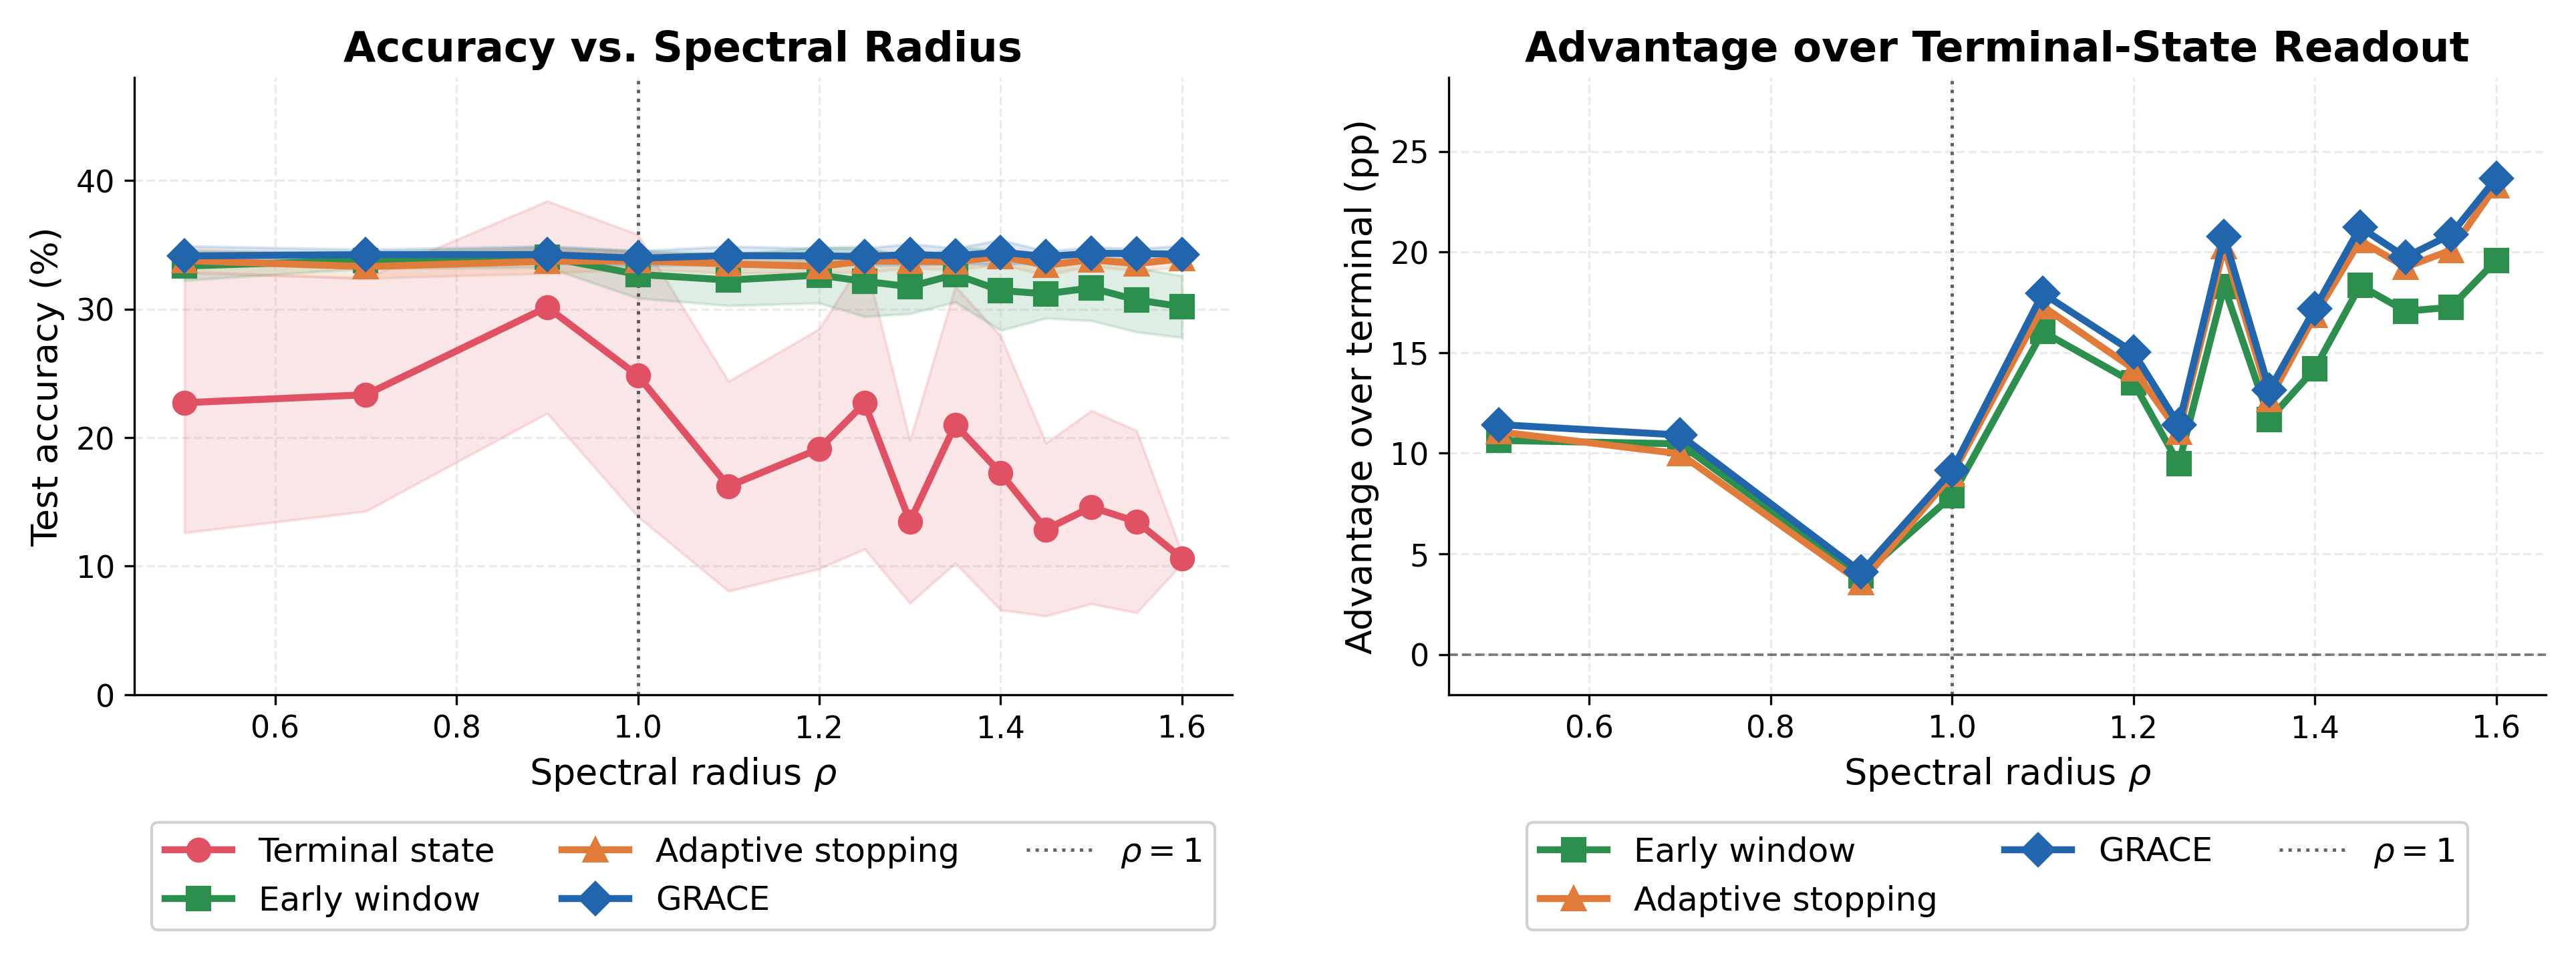
\includegraphics[width=\linewidth]{fig_cifar10_regime}
  \caption{\textbf{Pre-collapse regime on CIFAR-10.} Complex modReLU reservoir
  ($d=512$, $T=40$, 10 seeds, 5k/5k split). \emph{Left:} accuracy vs.\
  spectral radius $\sr$; shading shows $\pm$1 std across seeds.
  \emph{Right:} advantage of each non-terminal readout over the terminal
  state (pp). Terminal-state accuracy collapses to near chance at large $\sr$
  while \grace{} and early-window remain $20$--$24$~pp higher.}
  \label{fig:cifar10}
\end{figure}
\label{app:cifar_resnet18}

To separate the pre-collapse effect from the low absolute accuracy of the
raw-pixel CIFAR-10 reservoir, we repeat the CIFAR experiment using a stronger
frozen feature substrate. CIFAR-10 images are embedded with an
ImageNet-pretrained ResNet-18 penultimate layer~\citep{he2016deep}; a direct
ridge probe on these features achieves $85.2\%\pm0.1$ accuracy over 5
stratified 10k-train subsets and the full 10k test set. We then feed the
512-dimensional frozen features into the same complex modReLU reservoir
($d=512$, $T=40$), using exact eigenvalue spectral-radius rescaling.

The stable regime preserves the strong representation: at $\sr \leq 1.0$, all
readouts are near $84\%$. As $\sr$ increases, terminal readout collapses while
trajectory readouts remain near the frozen-feature baseline. At $\sr=1.6$,
terminal readout is $26.2\%\pm2.3$, while early-window is
$84.5\%\pm0.1$ and \grace{} is $84.0\%\pm0.1$.
The corresponding accuracy curves are shown in the main text in
\Cref{fig:cifar10_resnet18_main}; this appendix records the numerical setup
and endpoint-vs.-trajectory values.


\section{ESN GRACE Hyperparameter Sensitivity}
\label{app:esn_grace}

We evaluate four \grace{} hyperparameter configurations on the real-valued
tanh ESN (real ESN, $d=128$) across spectral radii, using the cross-system
results data (5 seeds per condition). The four configurations are defined
by $(\tau, \alpha)$: \texttt{t1.2\_a5} ($\tau=1.2$, $\alpha=5$),
\texttt{t1.2\_a10} ($\tau=1.2$, $\alpha=10$), \texttt{t1.5\_a5}
($\tau=1.5$, $\alpha=5$), and \texttt{t1.5\_a10} ($\tau=1.5$, $\alpha=10$).

\begin{table}[H]
\centering
\caption{\grace{} hyperparameter sensitivity on real-valued tanh ESN
(mean accuracy, 5 seeds). All four configurations substantially outperform
final-state readout across the unstable regime. The gains are robust to
hyperparameter choice within $\tau \in [1.2, 1.5]$, $\alpha \in [5,10]$.}
\label{tab:esn_grace}
\small
\begin{tabular}{l c cccc}
\toprule
$\sr$ & Final & $\tau{=}1.2,\alpha{=}5$ & $\tau{=}1.2,\alpha{=}10$ & $\tau{=}1.5,\alpha{=}5$ & $\tau{=}1.5,\alpha{=}10$ \\
\midrule
0.50 & $0.844$ & $0.843$ & $0.843$ & $0.843$ & $0.843$ \\
1.00 & $0.841$ & $0.843$ & $0.844$ & $0.842$ & $0.842$ \\
1.20 & $0.835$ & $0.843$ & $0.841$ & $0.842$ & $0.842$ \\
1.30 & $0.817$ & $0.843$ & $0.842$ & $0.841$ & $0.841$ \\
1.35 & $0.803$ & $0.843$ & $0.842$ & $0.841$ & $0.841$ \\
1.40 & $0.786$ & $0.843$ & $0.843$ & $0.840$ & $0.840$ \\
1.45 & $0.768$ & $0.843$ & $0.843$ & $0.841$ & $0.840$ \\
1.50 & $0.751$ & $0.842$ & $0.843$ & $0.840$ & $0.840$ \\
1.60 & $0.711$ & $0.843$ & $0.843$ & $0.840$ & $0.840$ \\
\bottomrule
\end{tabular}
\end{table}
\noindent
Key observation: all four configurations converge to similar performance,
confirming that the qualitative conclusions are insensitive to the precise
hyperparameter choice. The $\tau=1.2$ configurations are marginally stronger
at lower radii; the difference disappears in the deeply unstable regime
($\sr \geq 1.50$) where both $\tau$ values correctly identify the full
usable prefix.


\section{Grace Period Sweep}
\label{app:grace_period}

\Cref{app:grace_fig} distinguishes the formal quantity from the practical
proxy. The left panel plots the accuracy-defined grace period
$G(\rho,\alpha)$ for $\alpha \in \{0.65, 0.70, 0.75\}$; the right panel shows
the norm-ratio stopping time used as an online proxy. In these sweeps, both
shorten monotonically with spectral radius, but only the left panel is the
formal definition from \Cref{def:grace_period}. For $\alpha=0.70$, the
empirical grace period remains at the full horizon through $\rho \leq 1.20$,
then falls to $31.1$ at $\rho=1.40$, $20.2$ at $\rho=1.50$, and $15.2$ at
$\rho=1.60$. Using the mean norm-ratio proxy with $t_0=5$, a fitted
post-$t_0$ growth factor rises approximately linearly from
$1.013\pm0.024$ at $\rho=1.30$ to $1.126\pm0.012$ at $\rho=1.60$
(intermediate means: $1.056$ at $\rho=1.40$ and $1.100$ at $\rho=1.50$).

\begin{figure}[H]
  \centering
  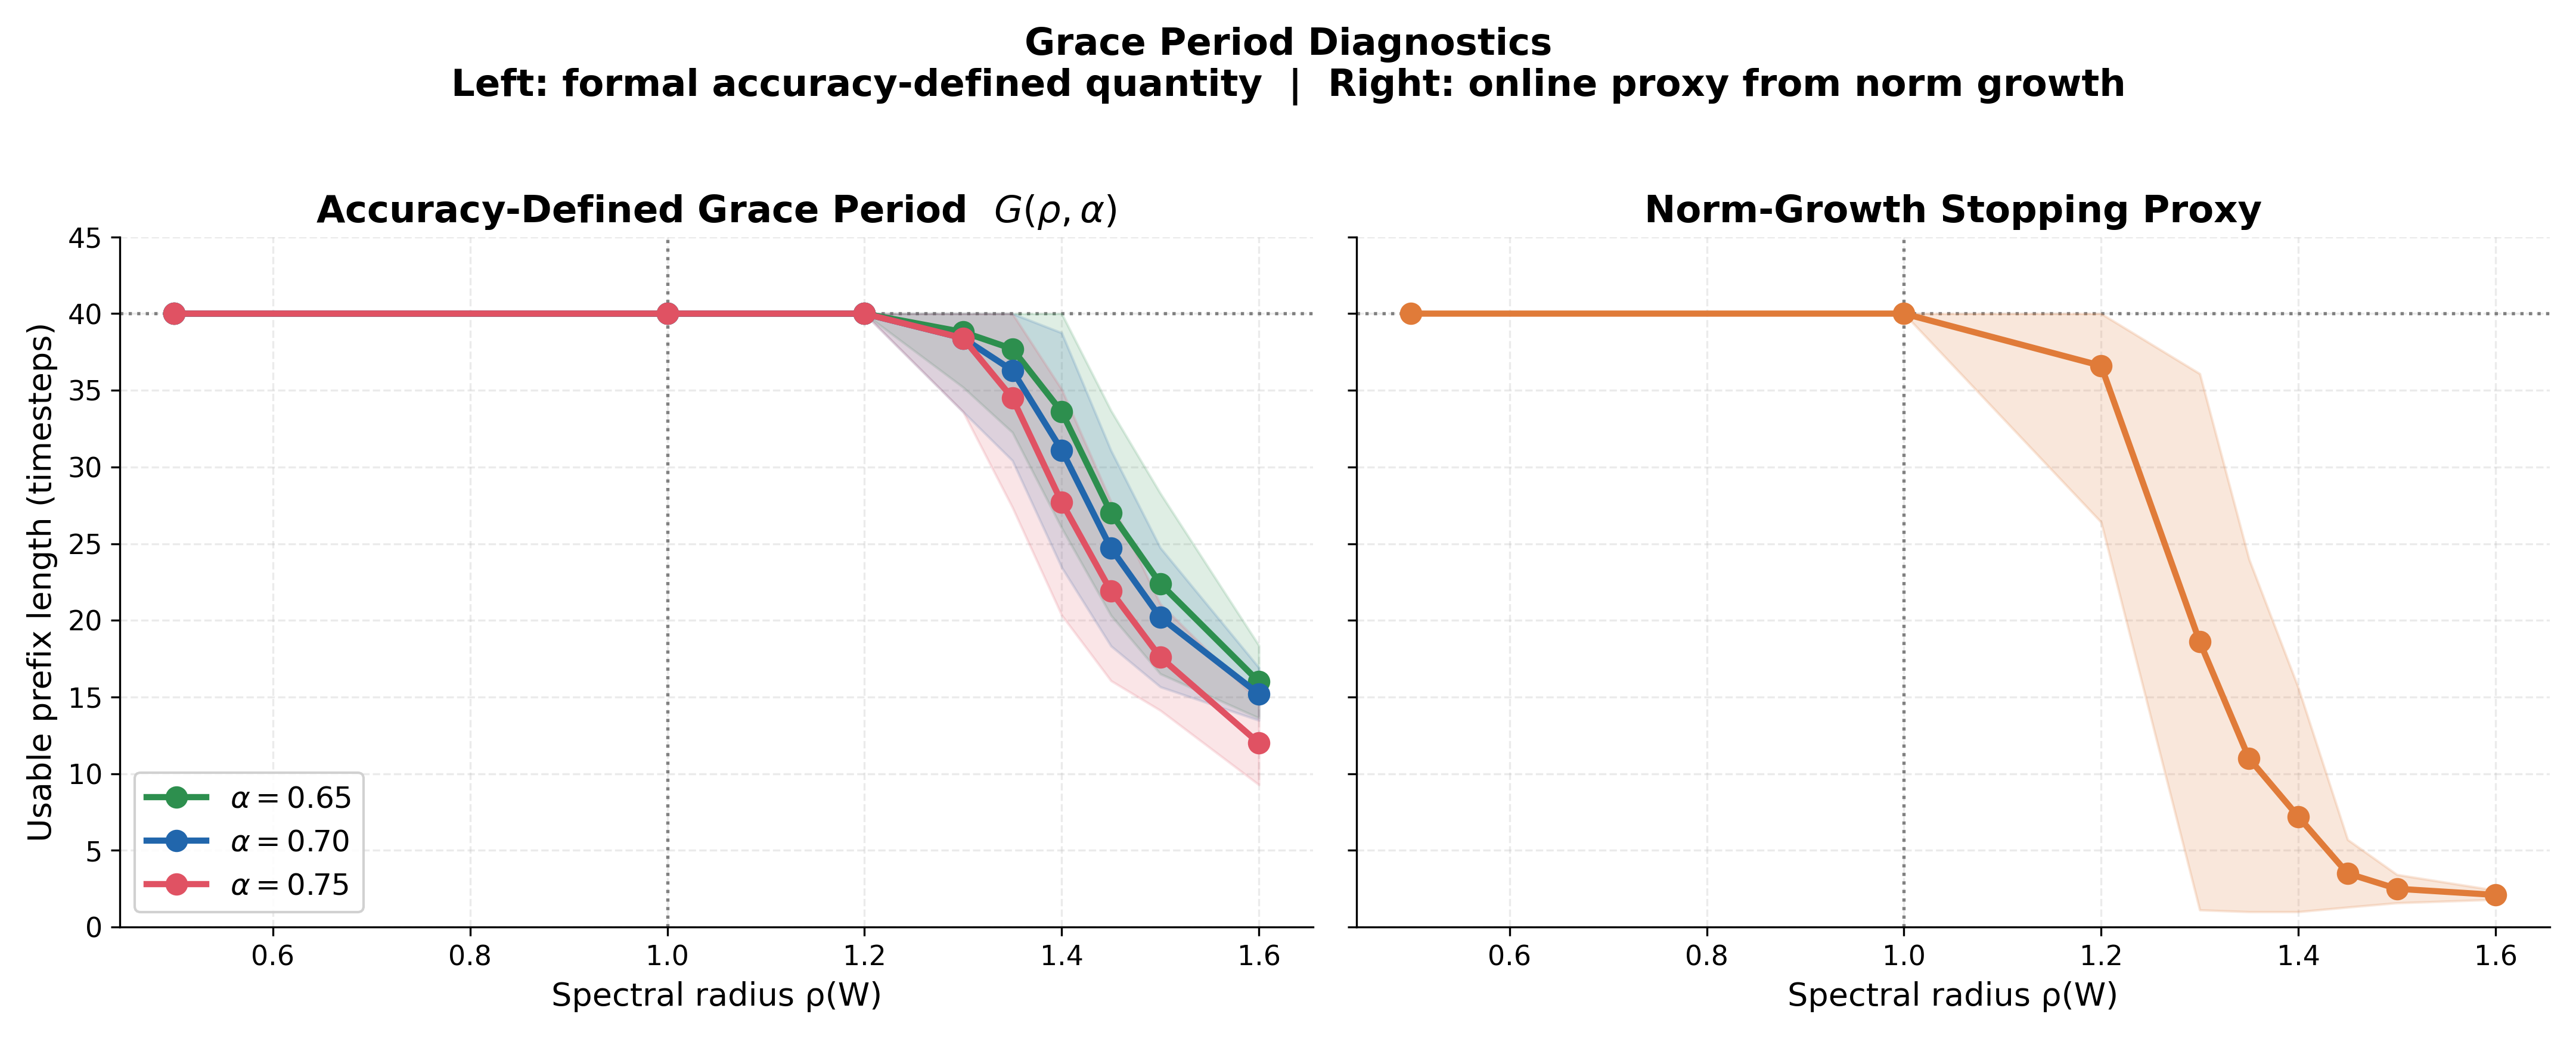
\includegraphics[width=\linewidth]{fig2_grace_period}
  \caption{\textbf{Formal grace period and norm-ratio proxy both shorten with instability.}
  \emph{Left:} the true accuracy-defined grace period $G(\rho,\alpha)$ for
  $\alpha \in \{0.65,0.70,0.75\}$, computed from per-timestep probe curves.
  \emph{Right:} the norm-ratio stopping time used as a practical online
  proxy. The proxy tracks the same qualitative shortening, but it is not
  interchangeable with the formal quantity. Shading shows $\pm1$ std across
  10 seeds.}
  \label{app:grace_fig}
\end{figure}

\section{Early-Window Sensitivity}
\label{app:k_sensitivity}

We fix $K=10$ in the main reservoir experiments. \Cref{fig:k_sensitivity}
shows that the main conclusion is not tied to this specific choice:
smaller windows are modestly stronger deep in the unstable regime, but
$K=10$ remains far above terminal-state readout and therefore serves as a
conservative, non-optimistic baseline rather than a cherry-picked optimum.
At $\rho=1.60$, for example, $K=1$ gives $82.2\%$, $K=10$ gives $80.9\%$,
and $K=20$ falls to $75.9\%$.

\begin{figure}[H]
  \centering
  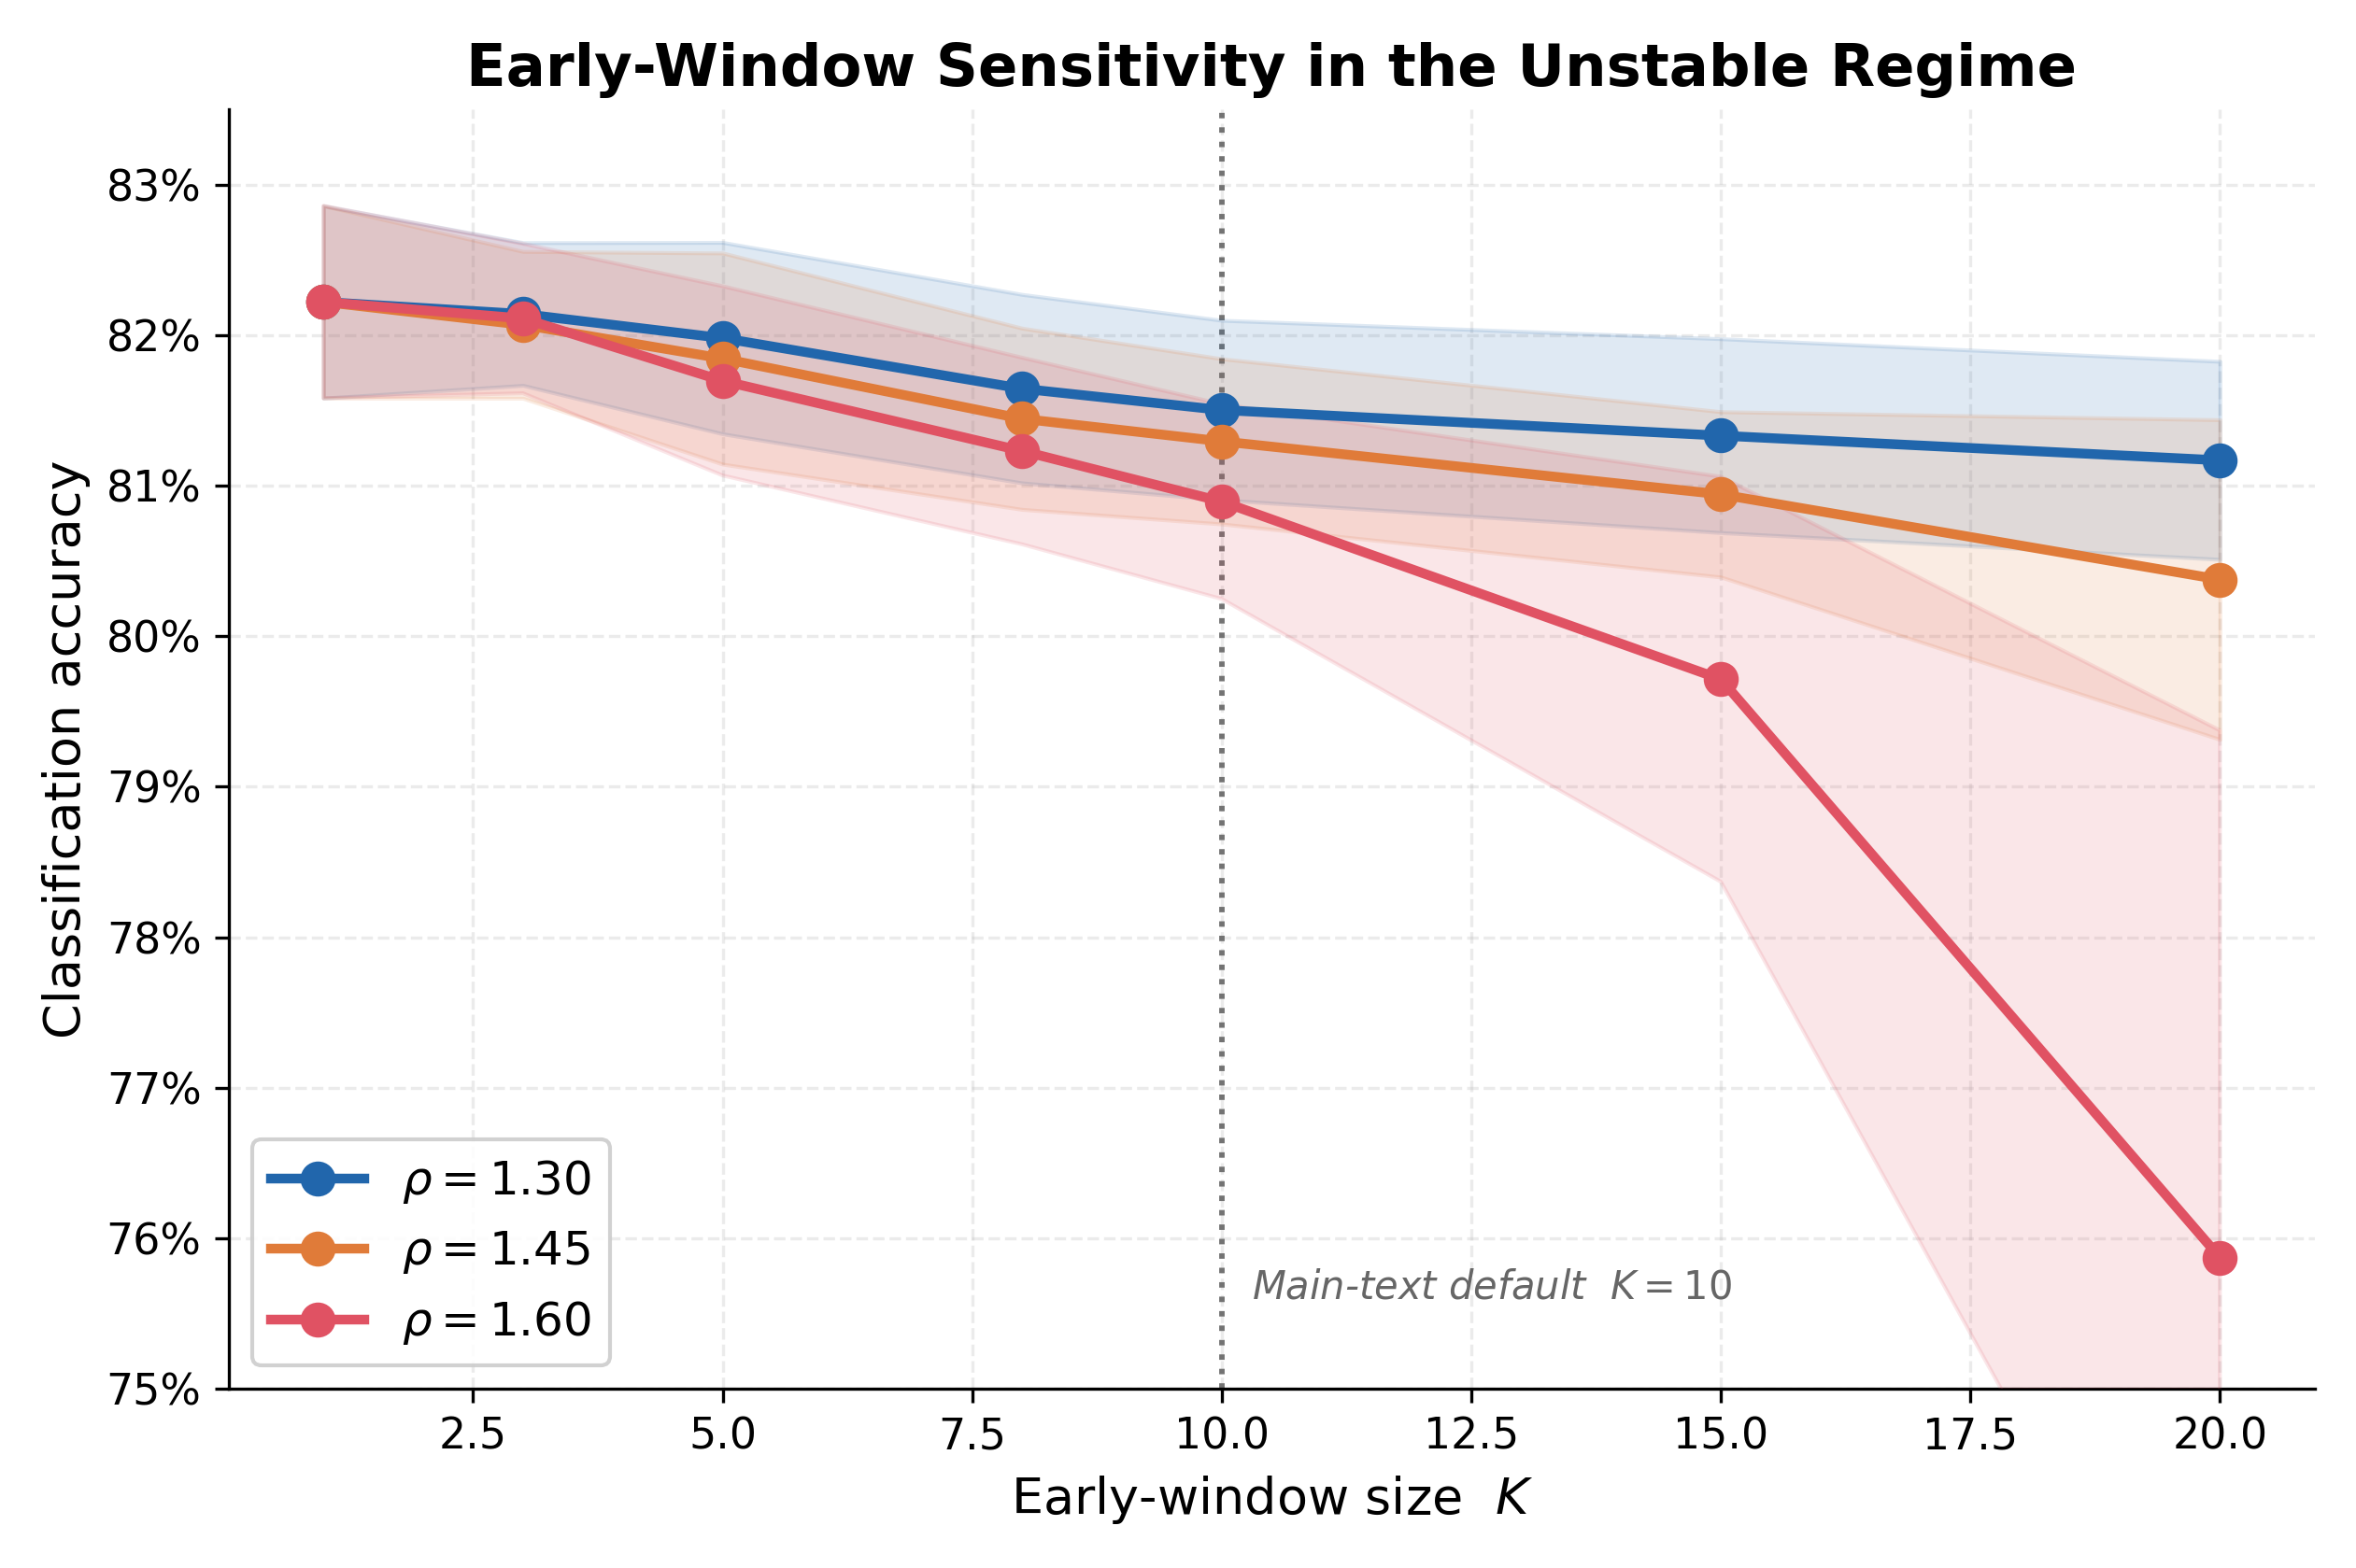
\includegraphics[width=0.72\linewidth]{fig7_k_sensitivity}
  \caption{\textbf{Early-window sensitivity over prefix length $K$.}
  Accuracy is shown for representative unstable radii
  $\rho \in \{1.30, 1.45, 1.60\}$ over $K \in \{1,3,5,8,10,15,20\}$.
  The fixed default $K=10$ is conservative: it is not optimal in the most
  unstable settings, but it still cleanly exhibits the pre-collapse regime.}
  \label{fig:k_sensitivity}
\end{figure}

\section{Reference-Radius Selection Audit}
\label{app:selection_protocol}

The main text uses fixed, simple defaults chosen before the final audit
($\tau_{\text{stop}}=1.5$ and $(\tau,\alpha)=(1.2,10)$), rather than settings
selected by sweeping the full spectral range. To check that the conclusion is
not an artefact of those defaults, we ran a lightweight post-hoc selection
audit at a single reference radius, $\rho=1.30$. The audit selected
$\tau_{\text{stop}}=1.0$ for adaptive stopping and $(\tau,\alpha)=(1.0,15)$
for \grace{}. These settings are slightly more aggressive, but freezing them
across the unstable band leaves the qualitative ranking unchanged: both
adaptive stopping and \grace{} remain near-flat and well above terminal-state
readout.

\begin{table}[H]
\centering
\caption{Frozen performance under the reference-radius selection audit.
Parameters are selected at $\rho=1.30$ and then held fixed elsewhere.}
\label{tab:selection_protocol}
\small
\begin{tabular}{l c c c}
\toprule
$\rho$ & Early ($K{=}10$) & Adaptive ($\tau_{\text{stop}}{=}1.0$) & \grace{} ($\tau{=}1.0,\alpha{=}15$) \\
\midrule
1.30 & 0.815 & 0.822 & 0.821 \\
1.40 & 0.813 & 0.822 & 0.820 \\
1.50 & 0.812 & 0.822 & 0.820 \\
1.60 & 0.809 & 0.822 & 0.820 \\
\bottomrule
\end{tabular}
\end{table}

\section{Noise Robustness Details}
\label{app:noise}

\Cref{fig:noise} shows per-seed accuracy in the fixed complex-modReLU reservoir
as a function of additive complex Gaussian dynamical noise at two representative spectral radii
($\rho = 1.4$ and $\rho = 1.5$). At each timestep, before the modReLU
activation, we add
\[
  \xi_t \in \C^d,\qquad
  \operatorname{Re}\xi_{t,j},\operatorname{Im}\xi_{t,j}
  \stackrel{\mathrm{i.i.d.}}{\sim}\mathcal{N}(0,\sigma_{\text{noise}}^2),
\]
using the same noise level during train- and test-feature extraction for the
linear probes.

\begin{figure}[H]
  \centering
  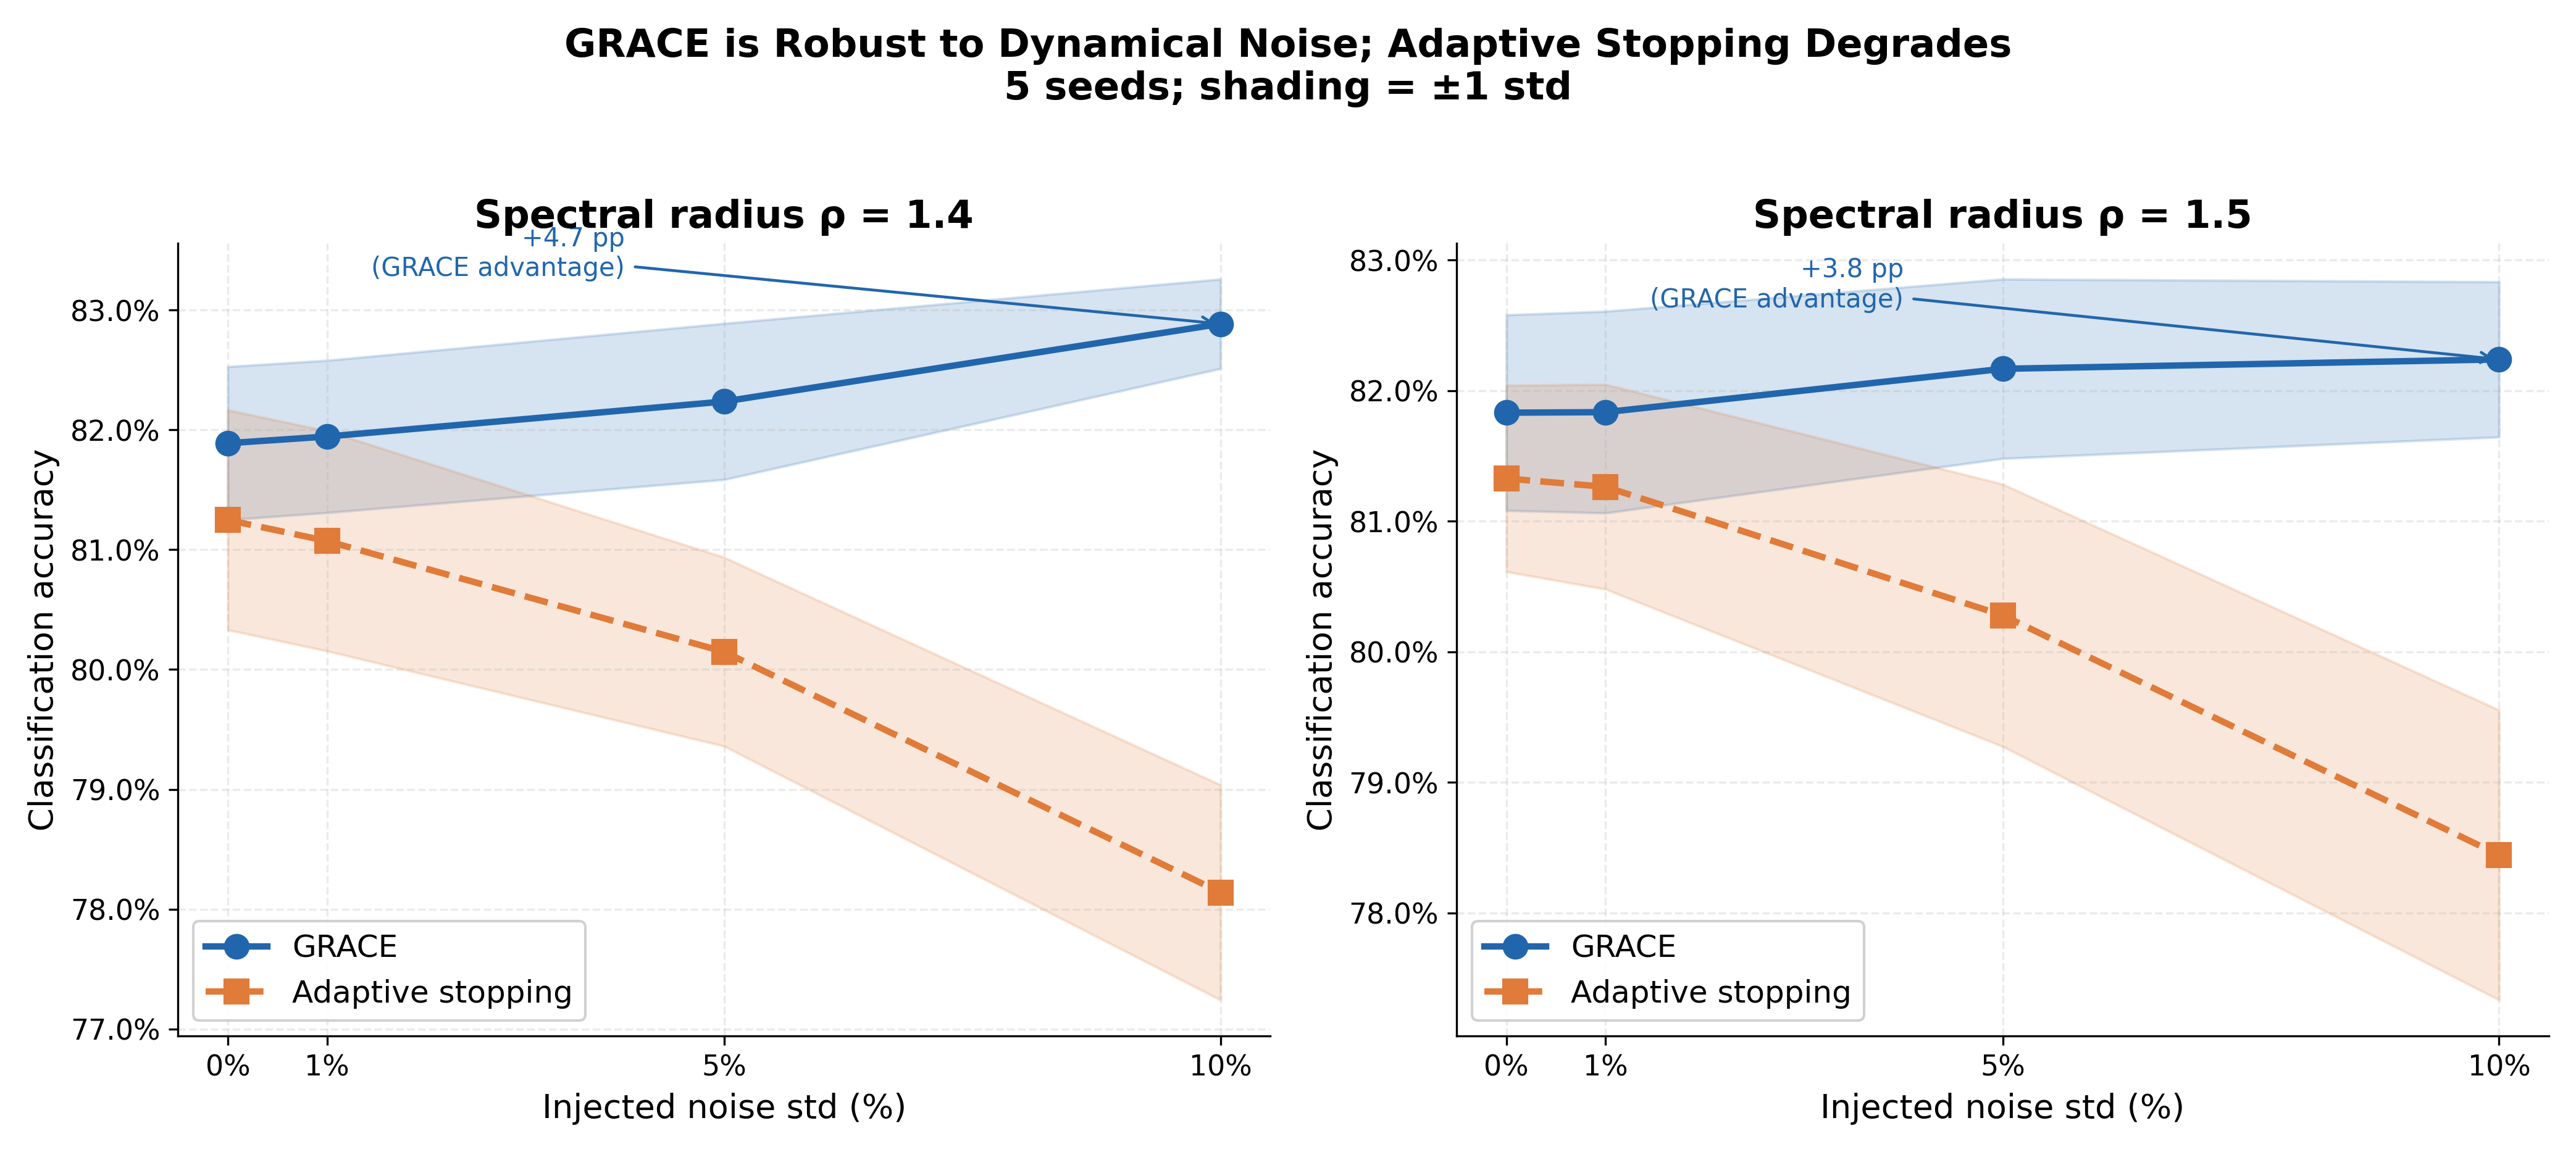
\includegraphics[width=\linewidth]{fig5_noise_robustness}
  \caption{\textbf{\grace{} is robust to dynamical noise; adaptive stopping
  degrades.} At both $\rho = 1.4$ (left) and $\rho = 1.5$ (right),
  \grace{} (blue) maintains accuracy as noise increases, while adaptive
  stopping (orange) falls 3--4 pp at $\sigma_\text{noise} = 0.10$
  (5 seeds; shading $= \pm 1$ std).}
  \label{fig:noise}
\end{figure}

Adaptive stopping degrades substantially: at $\sr = 1.40$ and $\sigma_\text{noise} = 0.10$,
accuracy drops from $81.2\%$ to $78.1\%$ ($-3.1$~pp). \grace{} is essentially unaffected at
$82.9\%$, a $+4.8$~pp advantage. At $\sr = 1.50$ the gap is $+3.8$~pp. All five \grace{}
runs at $\sr = 1.40$, $\sigma_\text{noise} = 0.10$ lie in $[82.2, 83.2]\%$ while all five
adaptive stopping runs lie in $[76.7, 79.4]\%$, with no overlap.

\section{Cross-System Taxonomy: Full Results}
\label{app:cross_system}

\Cref{fig:cross_system} shows the full per-radius accuracy curves for the
two nonlinear systems (complex modReLU and real ESN/tanh). The linear null
is summarised separately in \Cref{tab:cross_system}: spectral growth without
nonlinearity produces essentially no early-vs.-final gap.

\begin{figure}[H]
  \centering
  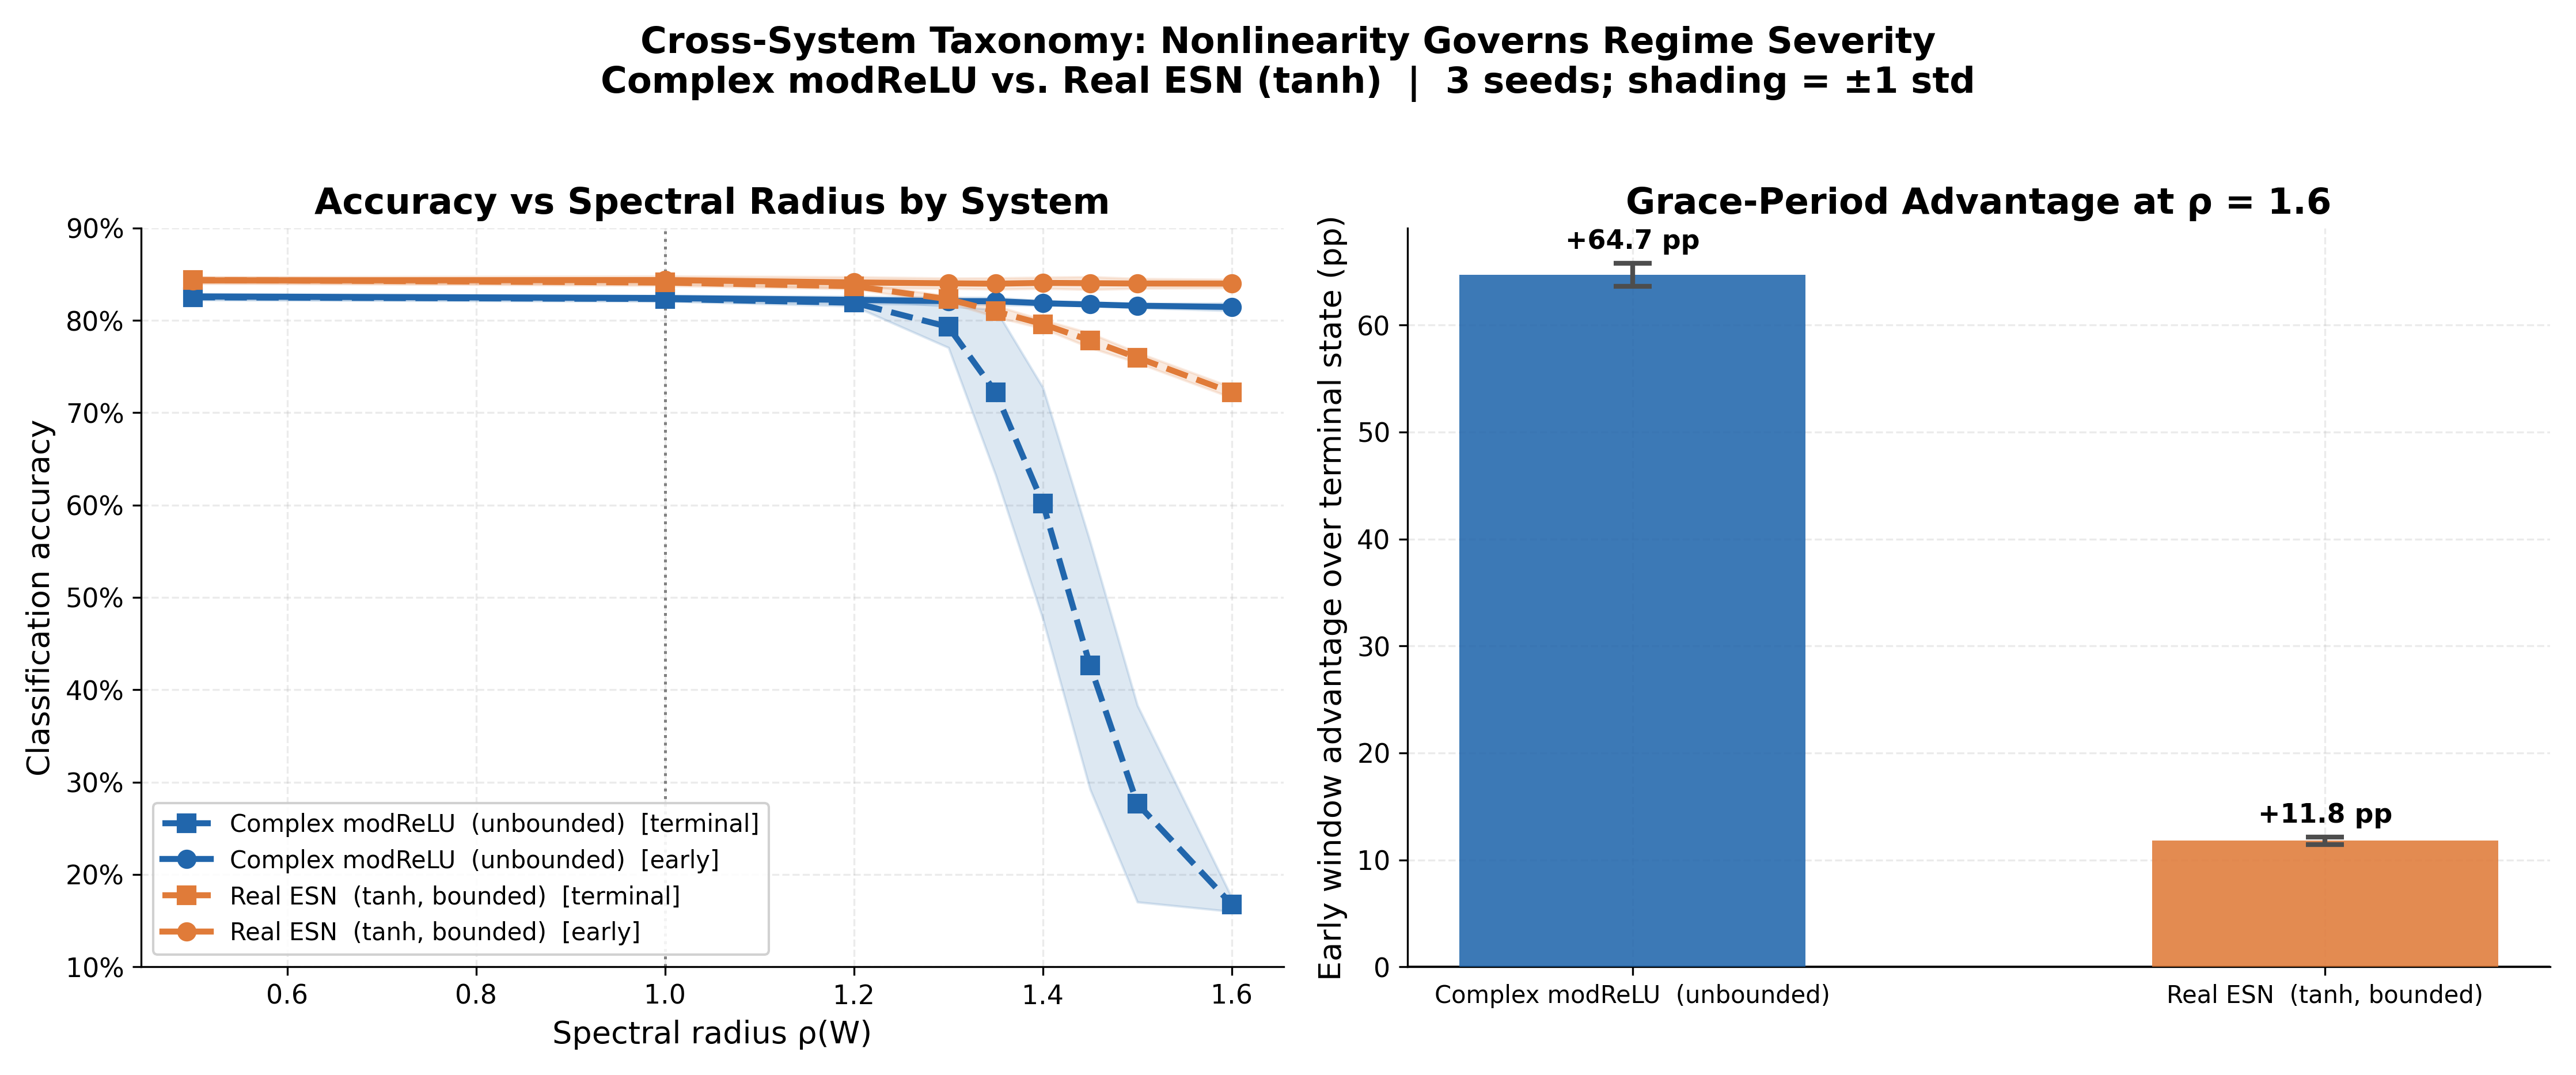
\includegraphics[width=\linewidth]{fig4_cross_system}
  \caption{\textbf{Cross-system taxonomy: nonlinearity governs regime severity.}
  \emph{Left:} accuracy vs spectral radius for complex modReLU (blue/dashed
  = terminal, blue/solid = early window) and real ESN/tanh (orange).
  \emph{Right:} grace-period advantage (Early $-$ Terminal, pp) at $\rho = 1.6$.
  The regime is dramatic in the unbounded system ($+64.7$~pp for
  modReLU) and moderate in the bounded system ($+11.8$~pp for tanh ESN),
  confirming that nonlinearity governs regime severity.}
  \label{fig:cross_system}
\end{figure}

\begin{table}[H]
\centering
\caption{Cross-system summary at $\rho = 1.6$. The linear system serves as a
null: spectral growth alone does not create a meaningful grace-period gap.}
\label{tab:cross_system}
\small
\begin{tabular}{l c c c c}
\toprule
System & Nonlinearity & Final & Early & Gap \\
\midrule
Complex modReLU & Unbounded & 0.167 & 0.814 & \textbf{+0.647} \\
Real ESN & Bounded (tanh) & 0.722 & 0.840 & +0.118 \\
Linear & None & 0.839 & 0.841 & +0.002 \\
\bottomrule
\end{tabular}
\end{table}

\section{Mechanism Diagnostics: Separability and Operator Amplification}
\label{app:mechanism_diag}

\Cref{fig:separability_time} provides a direct diagnostic for the mechanism
discussion in \Cref{sec:mechanism}. In the unstable regime, per-timestep
linear separability remains high over the early prefix and then collapses
sharply late in the rollout; the contractive and near-critical settings are
much flatter. This is consistent with the claim that useful input-imprinted
structure is available early, while late nonlinear distortion erodes it.

\begin{figure}[H]
  \centering
  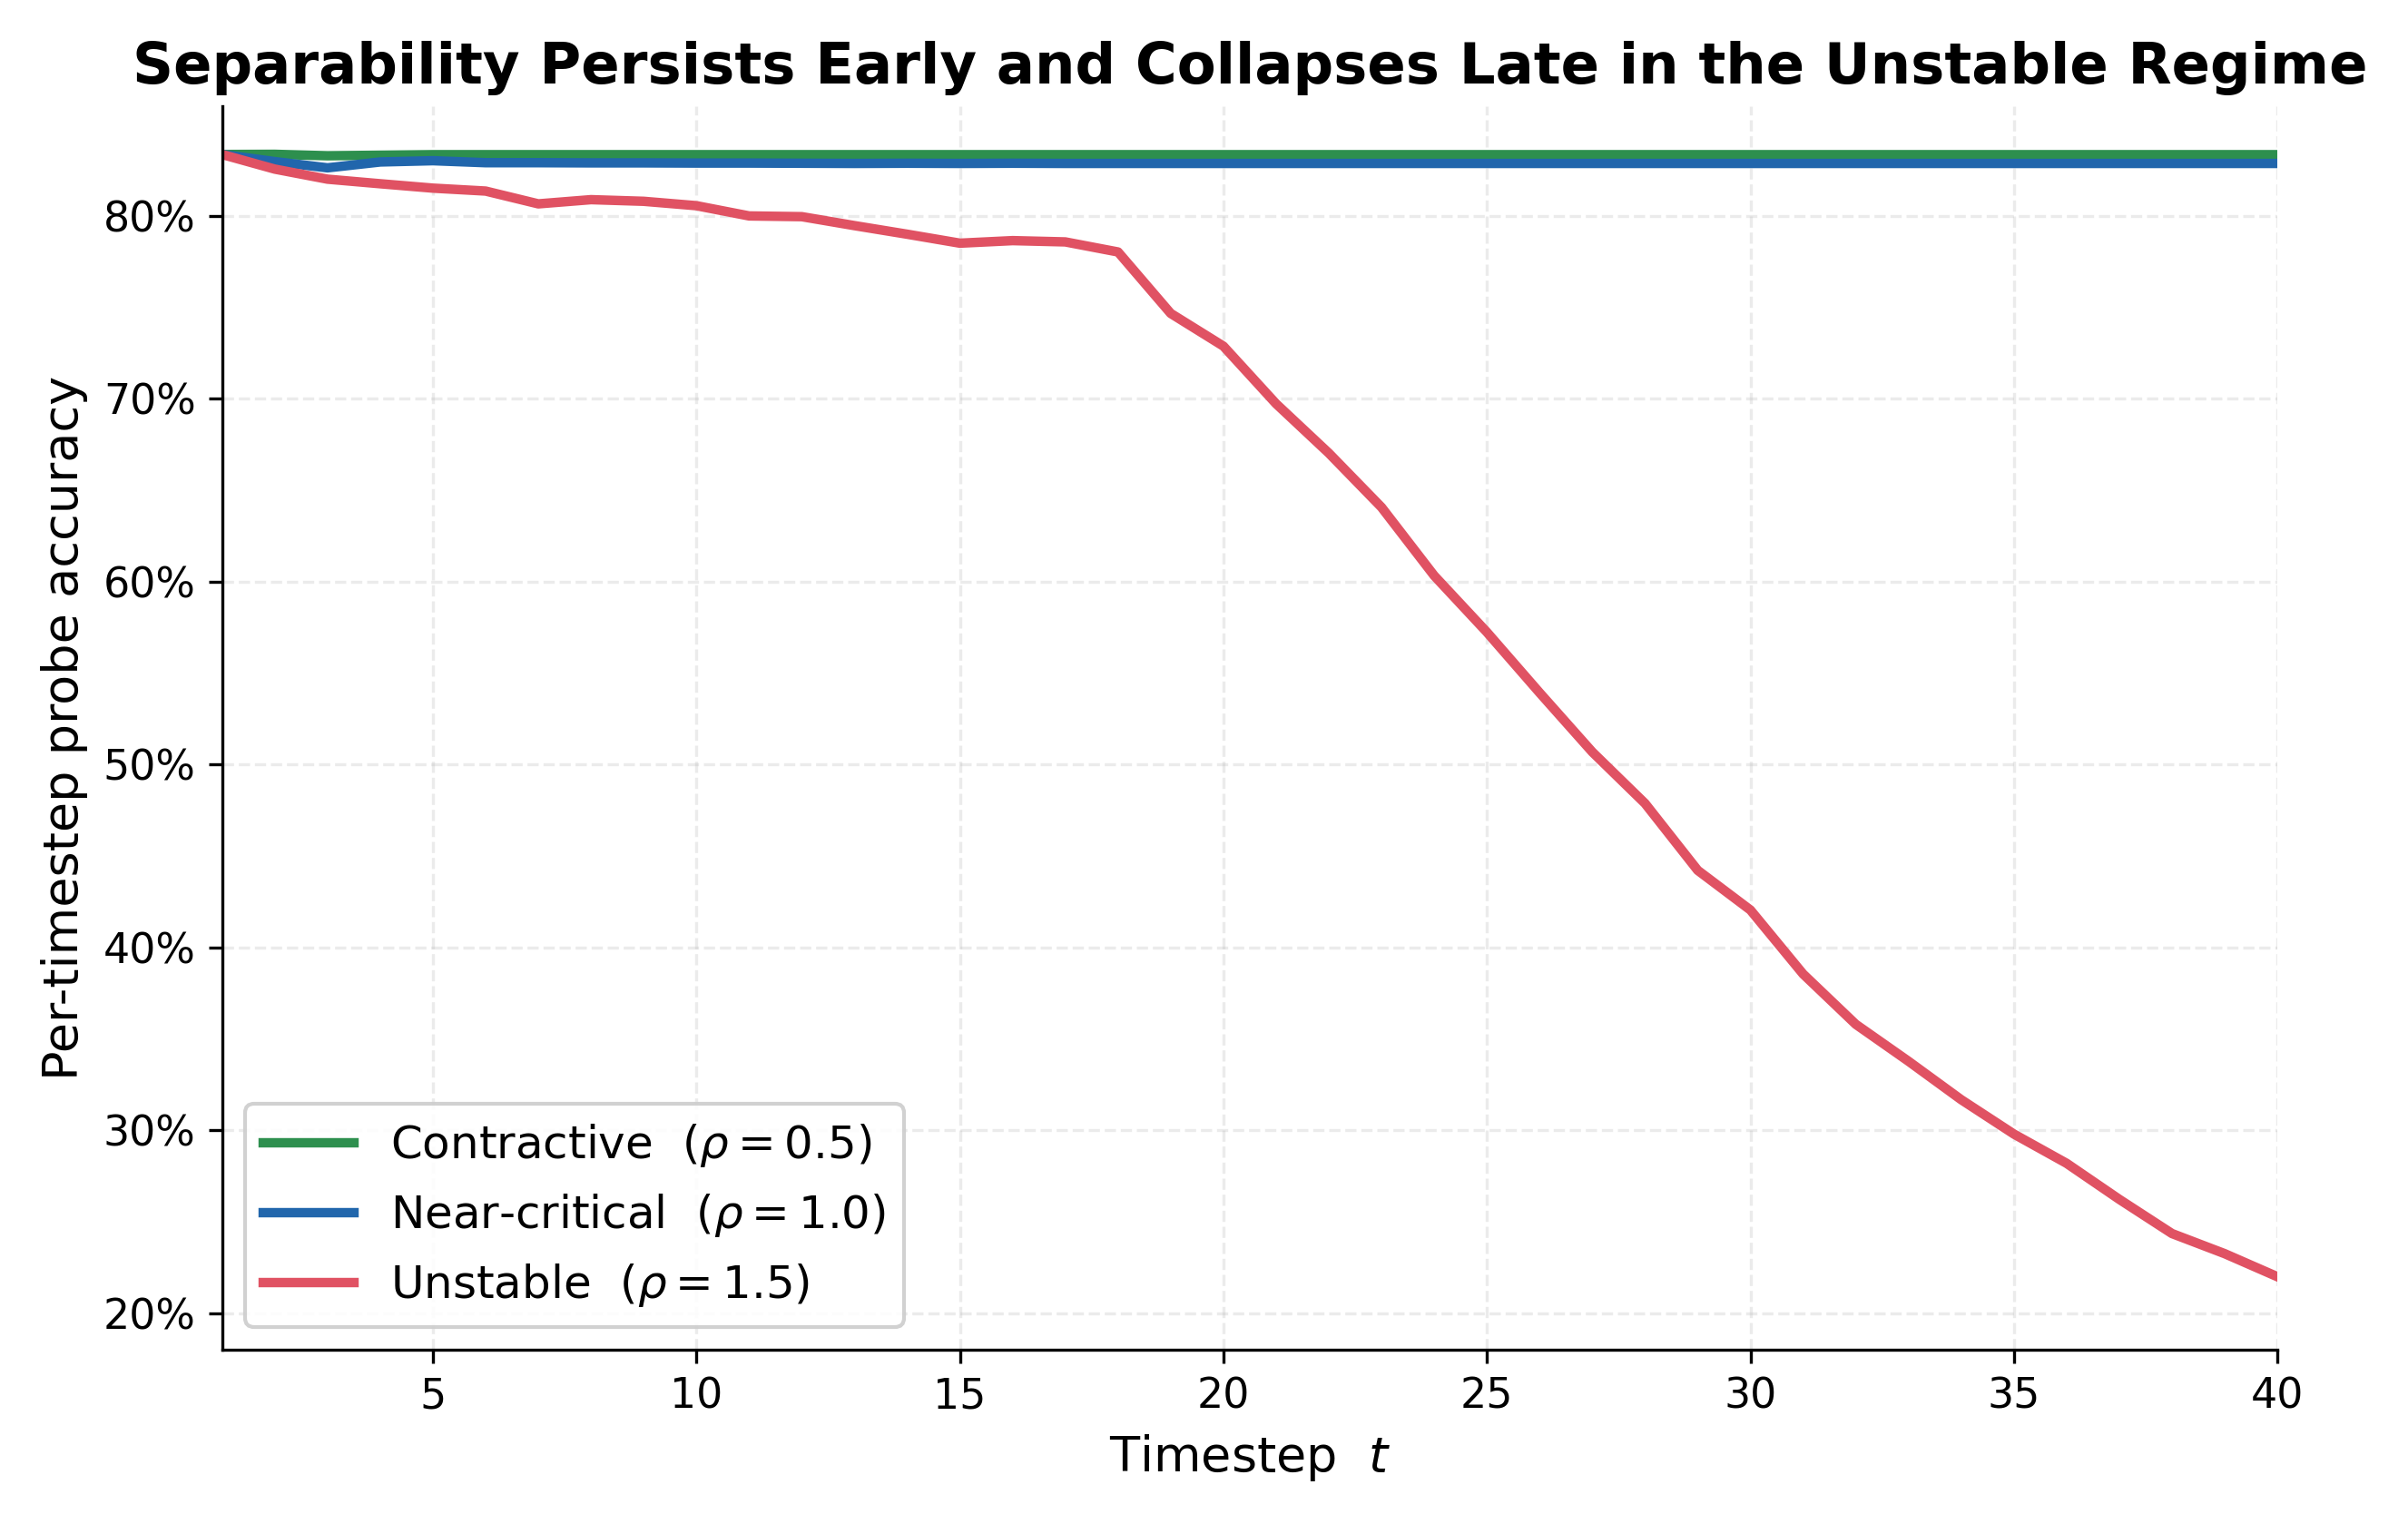
\includegraphics[width=0.72\linewidth]{fig8_separability_over_time}
  \caption{\textbf{Separability-over-time diagnostic.}
  Representative contractive ($\rho=0.5$), near-critical ($\rho=1.0$), and
  unstable ($\rho=1.5$) settings are shown. The unstable system retains a
  highly separable early prefix before collapsing sharply at later
  timesteps, consistent with a transiently usable computation window.}
  \label{fig:separability_time}
\end{figure}

\Cref{fig:operator_diagnostics} closes the theory-experiment loop for the
fixed-reservoir sweep by computing operator-level diagnostics on the actual
sampled matrices. Across the 10-seed complex-modReLU sweep, the finite-horizon
amplification proxy $\log_{10}\max_{t\le T}\|\bW^t\|_2$ correlates strongly
with shorter grace periods ($r=-0.75$) and larger $\grace{}$-over-final gains
($r=0.76$). Within fixed $\rho$, the scaled-Kreiss estimate $K_\rho(\bW)$ still
explains residual seed-to-seed variation in the gap ($r=0.39$), showing that
radial growth dominates across the sweep while non-normality modulates residual
severity. The bottom panel shows why amplification alone is not enough: the
real tanh ESN and the linear null have nearly identical operator envelopes, yet
only the nonlinear system develops a meaningful readout gap.

\begin{figure}[H]
  \centering
  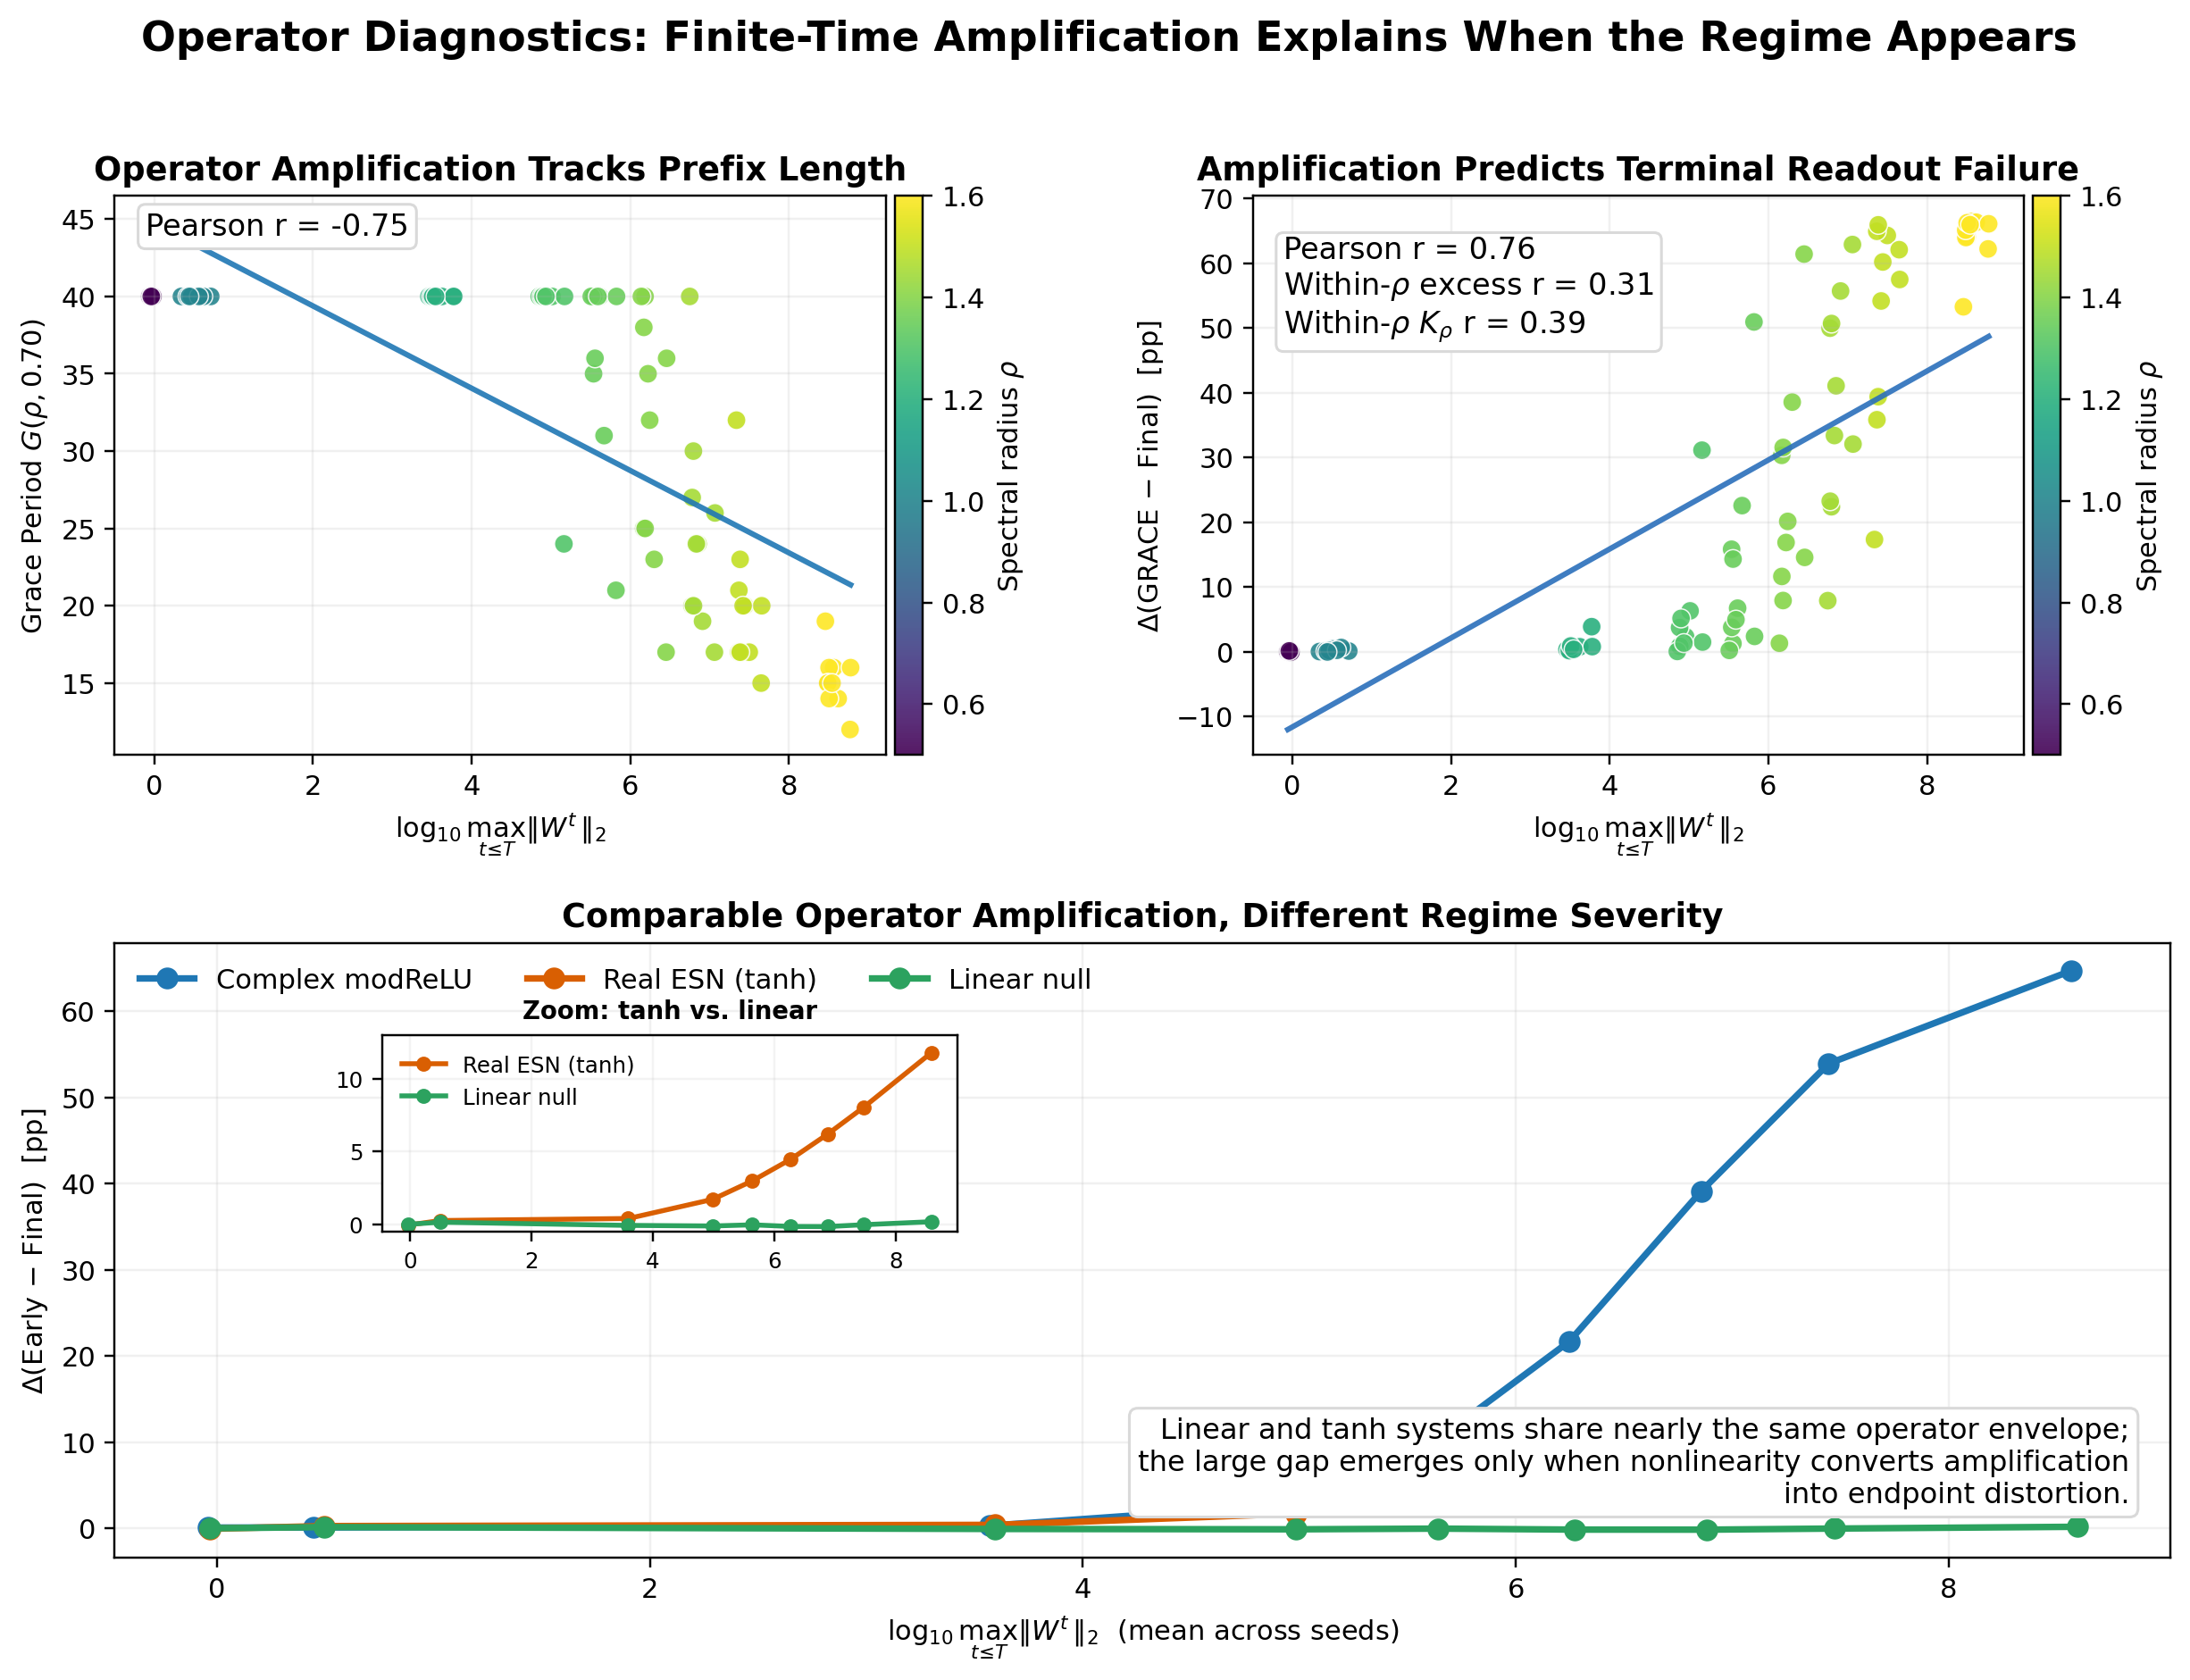
\includegraphics[width=0.96\linewidth]{fig10_operator_diagnostics}
  \caption{\textbf{Operator diagnostics on the actual reservoir sweep.}
  \emph{Top left:} finite-horizon amplification tracks grace-period shortening
  across the 10-seed complex-modReLU sweep ($r=-0.75$).
  \emph{Top right:} the same amplification proxy predicts $\grace{}$-over-final
  improvement ($r=0.76$); after factoring out spectral-radius trends, residual
  within-$\rho$ variation still correlates with scaled-Kreiss non-normality
  ($r=0.39$).
  \emph{Bottom:} across systems at $\rho=1.6$, the tanh ESN and linear null
  have nearly identical amplification envelopes, but only the nonlinear system
  exhibits a substantial gap. Across these tested systems, finite-time
  amplification tracks regime severity but is not sufficient for endpoint
  distortion; comparable amplification yields a substantial gap only in
  the nonlinear system.}
  \label{fig:operator_diagnostics}
\end{figure}

\section{DEQ-Style Relevance Check}
\label{app:deq}

We include a small DEQ-style relevance check as a separate appendix
experiment, not as a replot of the trained LeakyReLU sweep in
\Cref{sec:trained_system}. The model is a $d=128$ tanh fixed-point classifier
on flattened MNIST,
$z_{k+1}=\tanh(\lambda \bW z_k+\bU x+b)$, trained on a 5k/2k split for
25 epochs with Adam at learning rate $10^{-3}$, $K_{\rm train}=10$, and
$\lambda_{\rm train}=0.80$. At evaluation we run $K_{\rm test}=50$ Picard
iterations over $\lambda_{\rm test}\in\{0.80,\ldots,1.40\}$ and score the
same final, early-window, adaptive, and \grace{} readouts using
RidgeClassifierCV probes on a half-split of the held-out set. This lower-capacity
check is not meant to match the absolute accuracies in \Cref{tab:e6}; it only
tests whether an endpoint-vs.-trajectory mismatch can also appear near a
fixed-point solver's stability boundary. \Cref{fig:deq_relevance} shows a
modest but consistent early-window advantage of roughly $1$--$1.5$~pp over
final-iterate readout across the tested gain range, with \grace{} remaining
close but slightly weaker in this setting.

\begin{figure}[H]
  \centering
  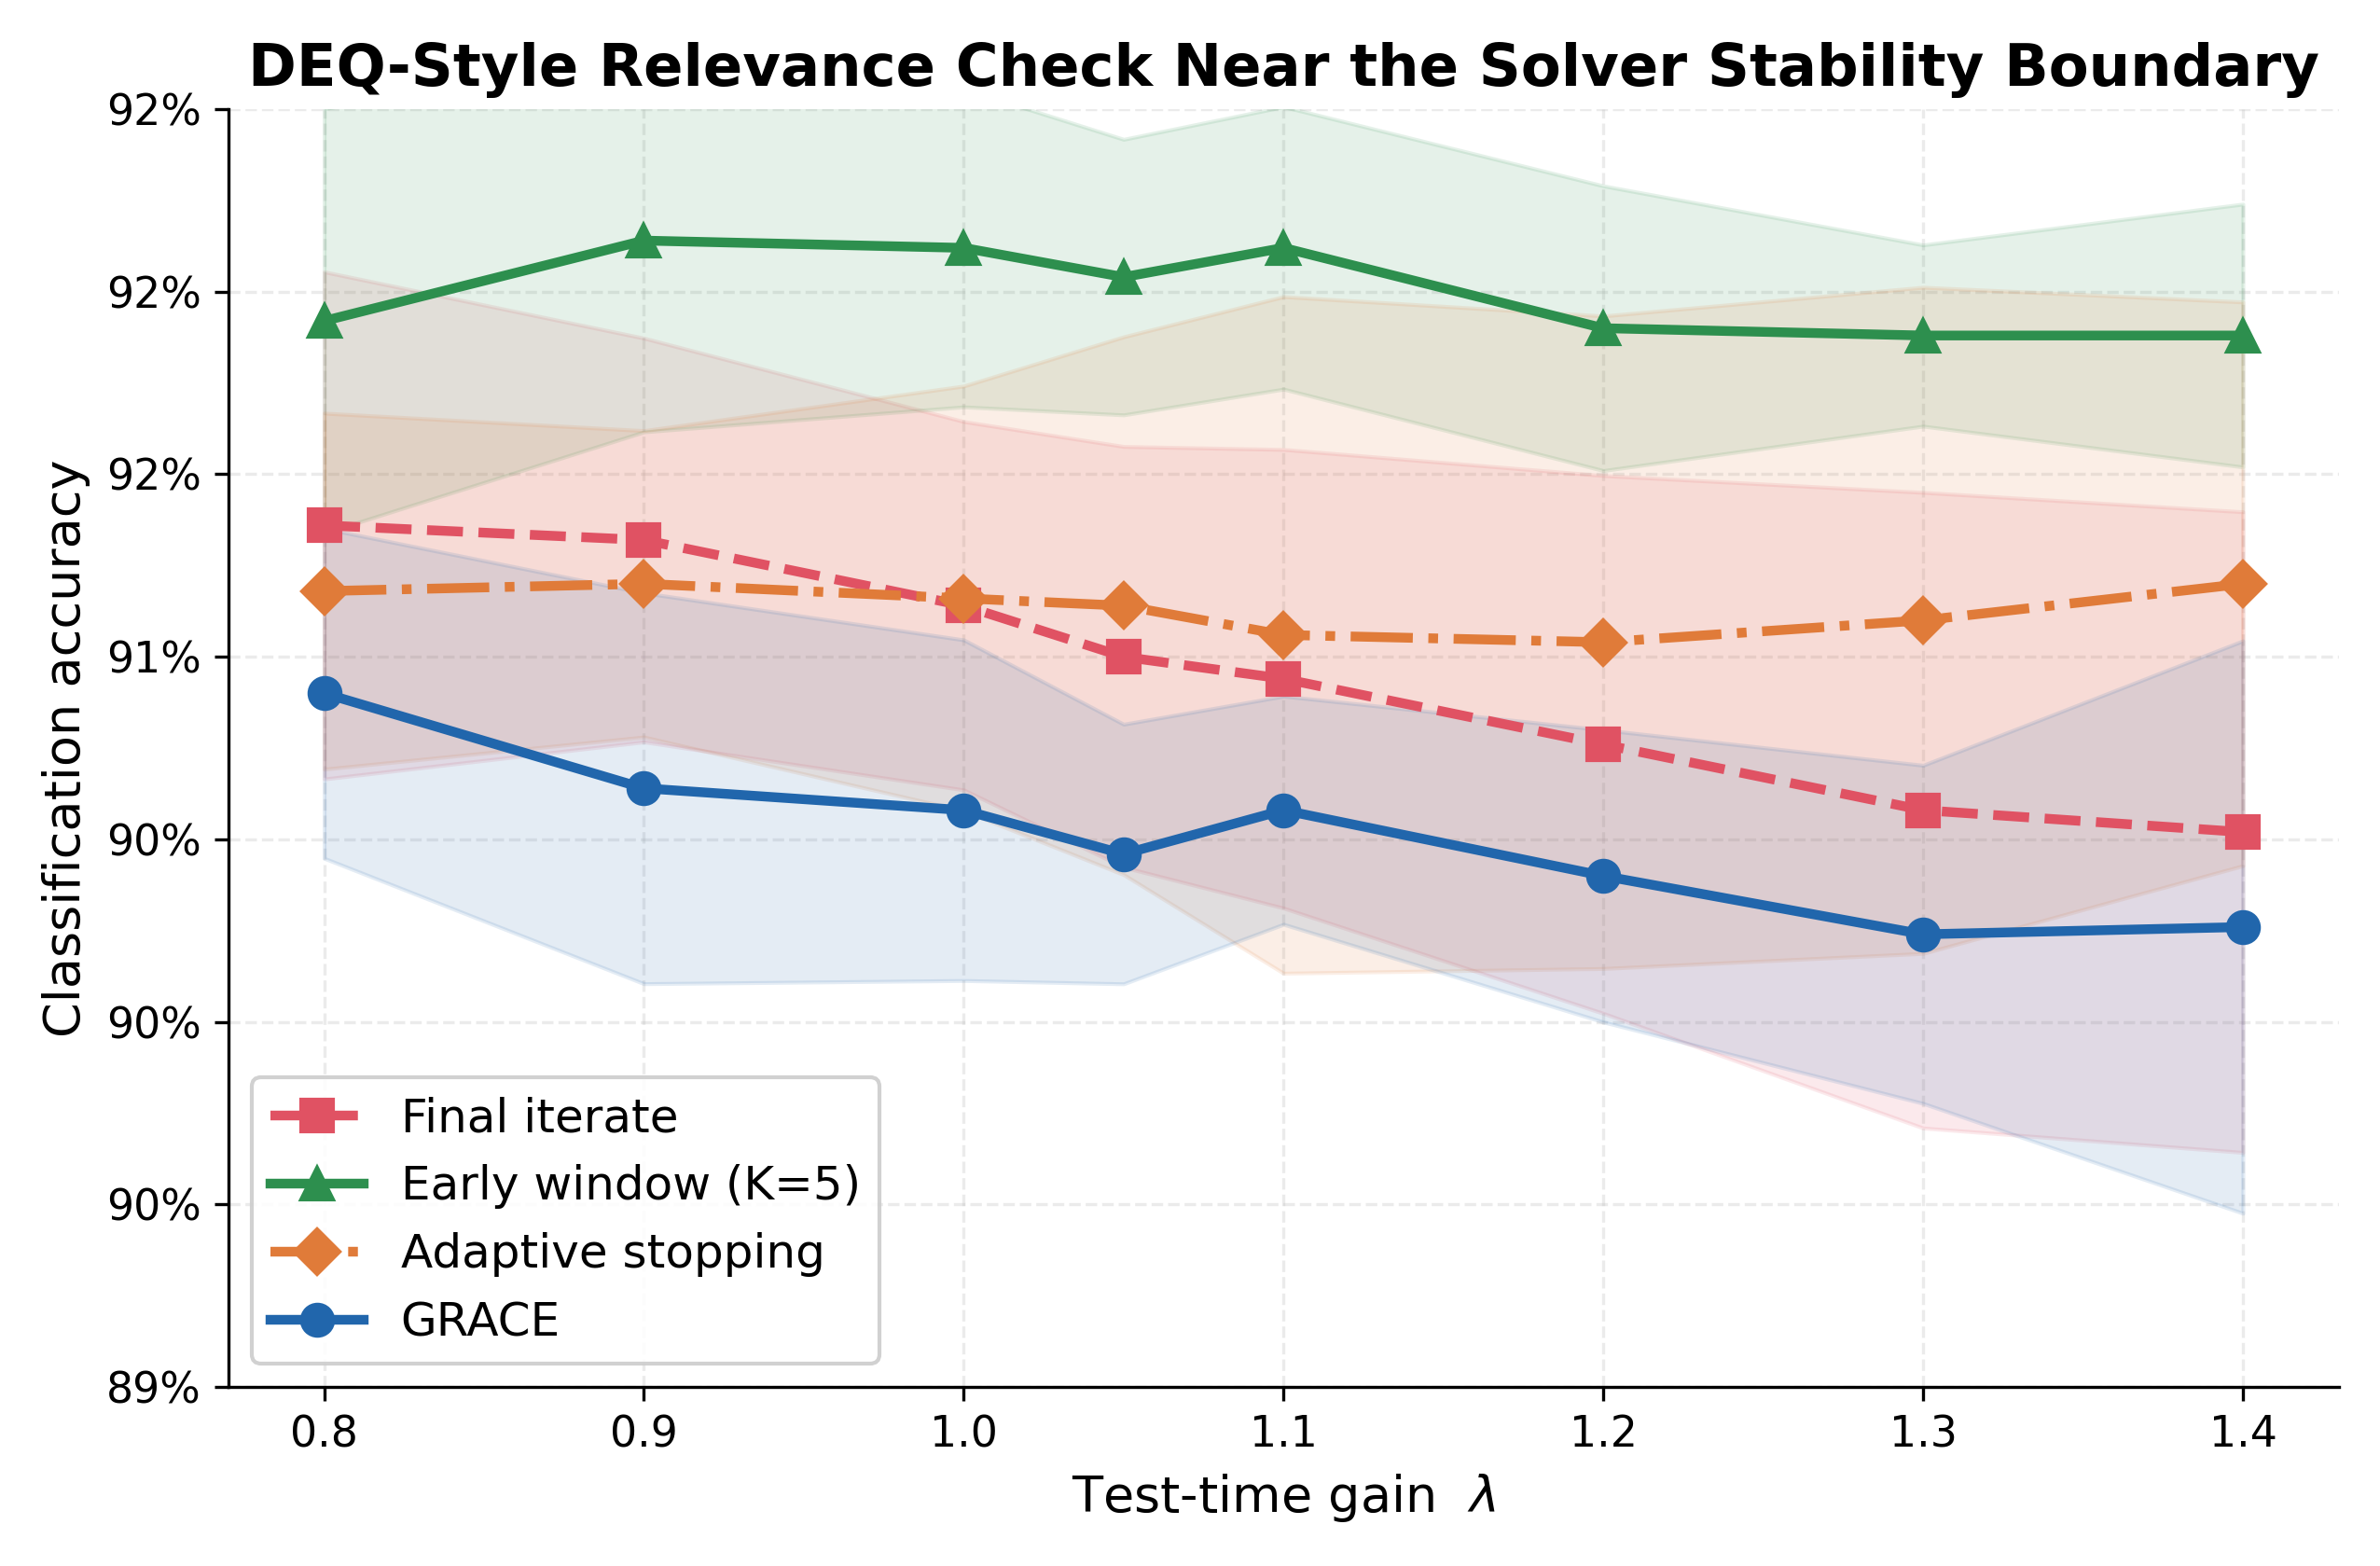
\includegraphics[width=0.72\linewidth]{fig9_deq_relevance}
  \caption{\textbf{Limited DEQ-style relevance check.}
  In a separate $d=128$ tanh fixed-point MNIST classifier, early-window readout
  retains a modest advantage over the final iterate near the solver stability
  boundary, while adaptive stopping stays close and \grace{} remains slightly
  weaker. We report this only as an appendix-level relevance check for
  iterative/fixed-point models.}
  \label{fig:deq_relevance}
\end{figure}

\section{Sequential CIFAR-10 LSTM Check}
\label{app:seq_cifar_lstm}

We include a second trained-system check on a standard gated recurrent
architecture. CIFAR-10 images are presented as row sequences
($32$ timesteps, $96$ input dimensions per row) to a 512-hidden-unit LSTM
trained end-to-end on terminal-state cross-entropy. To avoid confounding early
readout with missing pixels, all readouts are taken only after the full image
has been processed: we run a 40-step zero-input post-image settling trajectory
at train time ($\lambda_{\rm train}=1.0$) and at test time sweep the recurrent
gain $\lambda_{\rm test}$. Training uses 10k CIFAR-10 examples, 2k test
examples, AdamW with learning rate $10^{-3}$ and weight decay $10^{-4}$, batch
size 64, 30 epochs, and 3 seeds. Readout accuracies use the same
RidgeClassifierCV probe protocol on final, early-window, adaptive, and
\grace{} features; the dense single-timestep audit uses a fixed ridge
regularisation $\alpha_{\rm ridge}=1.0$ for computational tractability.

\Cref{fig:seq_cifar_lstm,fig:seq_cifar_lstm_timestep,tab:seq_cifar_lstm} show
the same qualitative pattern as the trained LeakyReLU sweep, at smaller
magnitude: terminal readout degrades with test-time gain, while early-window
readout degrades more slowly. At $\lambda_{\rm test}=2.0$, final accuracy is
$0.361\pm0.007$, early-window is $0.396\pm0.009$ ($+3.5$ pp), and \grace{} is
$0.384\pm0.009$ ($+2.3$ pp). Adaptive stopping mostly matches the terminal
state, consistent with a bounded gated recurrent system in which the
norm-threshold signal is weak. A separate single-timestep probe audit confirms
an accuracy-defined prefix shortening: for accuracy threshold $0.40$, the
measured prefix lengths at $\lambda_{\rm test}\in\{1.0,1.6,2.0\}$ are
$40$, $27$, and $2$ post-input settling steps, respectively.

\begin{figure}[H]
  \centering
  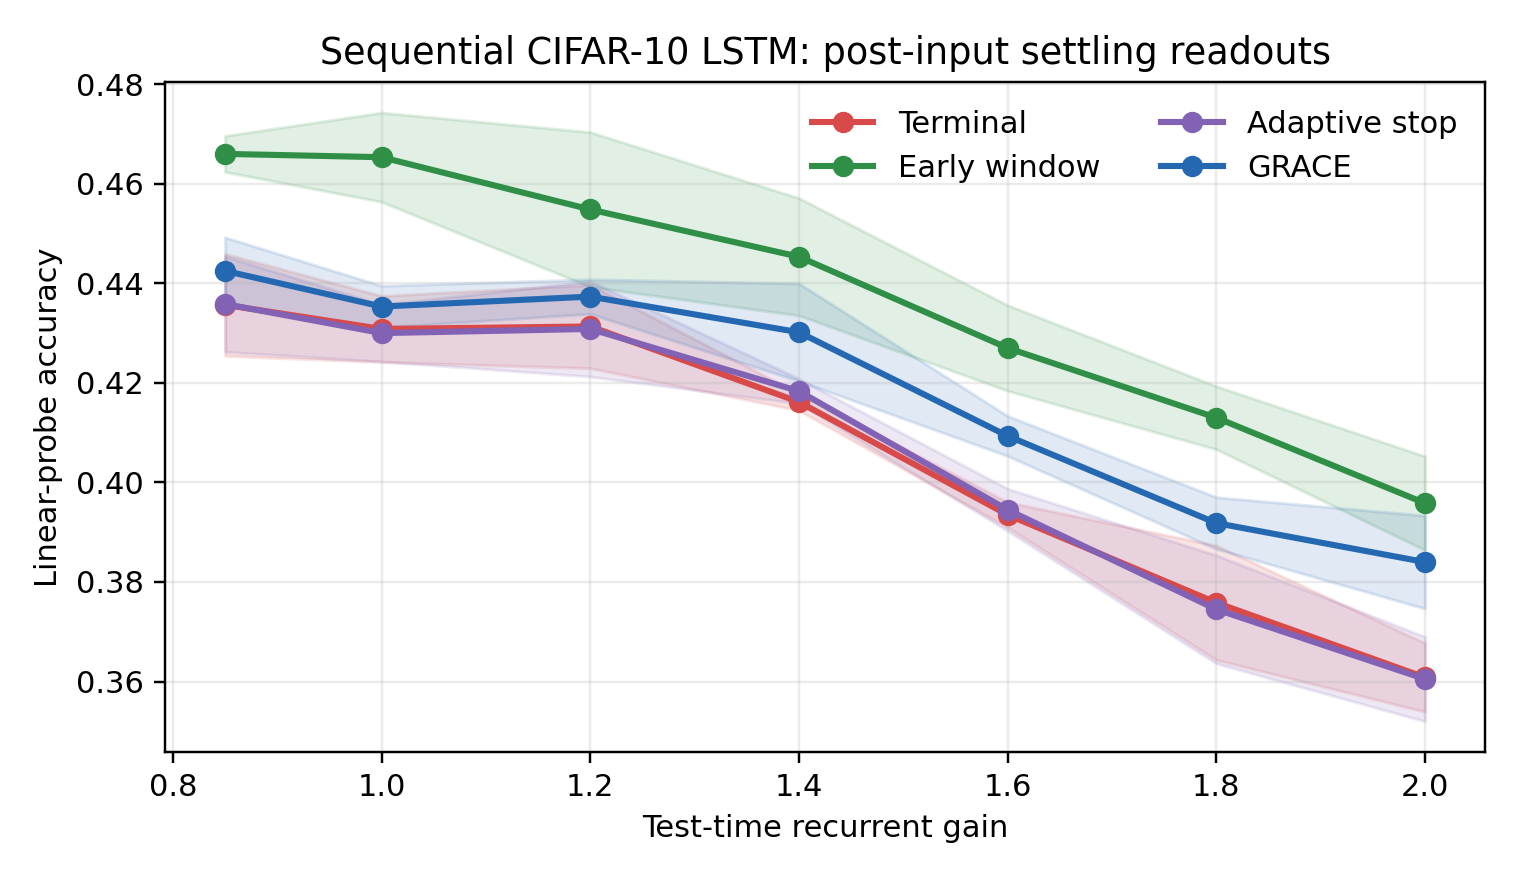
\includegraphics[width=0.72\linewidth]{fig13_seq_cifar10_lstm}
  \caption{\textbf{Sequential CIFAR-10 LSTM post-input settling check.}
  After the full image has been processed, a trained 512-unit LSTM is run for a
  40-step zero-input settling trajectory while recurrent gain is swept at test
  time. Terminal readout degrades with gain; early-window and \grace{} remain
  higher at large gains (3 seeds).}
  \label{fig:seq_cifar_lstm}
\end{figure}

\begin{figure}[H]
  \centering
  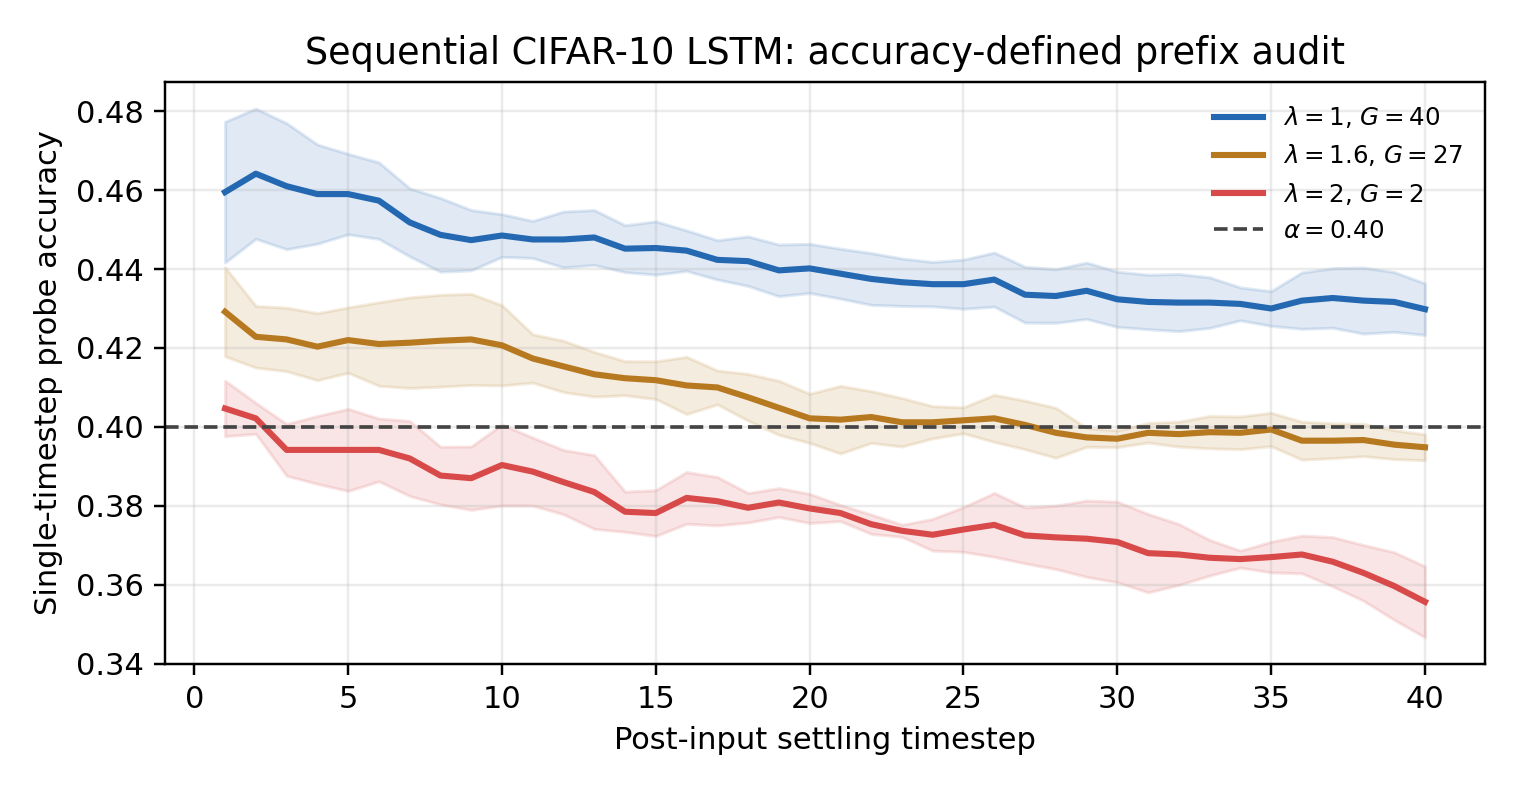
\includegraphics[width=0.72\linewidth]{fig14_seq_cifar10_lstm_timestep_audit}
  \caption{\textbf{Accuracy-defined prefix audit for the sequential CIFAR-10
  LSTM.} We fit a separate linear probe at each post-input settling timestep
  for three test-time gains. At accuracy threshold $0.40$, the usable prefix
  shortens from the full 40-step trajectory at $\lambda=1.0$ to 27 steps at
  $\lambda=1.6$ and 2 steps at $\lambda=2.0$ (3 seeds).}
  \label{fig:seq_cifar_lstm_timestep}
\end{figure}

\begin{table}[H]
\centering
\caption{Sequential CIFAR-10 LSTM readout accuracy (mean $\pm$ std, 3 seeds).
The effect is modest, as expected for a bounded gated recurrent architecture,
but the endpoint-vs.-trajectory gap grows at high test-time gain.}
\label{tab:seq_cifar_lstm}
\small
\begin{tabular}{l c c c c c}
\toprule
$\lambda_{\rm test}$ & Final & Early & Adaptive & \grace{} & Early$-$Final \\
\midrule
0.85 & $0.436{\pm}0.010$ & $0.466{\pm}0.004$ & $0.436{\pm}0.010$ & $0.443{\pm}0.007$ & $+3.0$ pp \\
1.00 & $0.431{\pm}0.007$ & $0.465{\pm}0.009$ & $0.430{\pm}0.006$ & $0.435{\pm}0.004$ & $+3.5$ pp \\
1.20 & $0.431{\pm}0.008$ & $0.455{\pm}0.016$ & $0.431{\pm}0.010$ & $0.437{\pm}0.003$ & $+2.4$ pp \\
1.40 & $0.416{\pm}0.002$ & $0.445{\pm}0.012$ & $0.418{\pm}0.002$ & $0.430{\pm}0.010$ & $+2.9$ pp \\
1.60 & $0.394{\pm}0.003$ & $0.427{\pm}0.009$ & $0.395{\pm}0.004$ & $0.409{\pm}0.004$ & $+3.4$ pp \\
1.80 & $0.376{\pm}0.011$ & $0.413{\pm}0.006$ & $0.375{\pm}0.011$ & $0.392{\pm}0.005$ & $+3.7$ pp \\
2.00 & $0.361{\pm}0.007$ & $0.396{\pm}0.009$ & $0.361{\pm}0.008$ & $0.384{\pm}0.009$ & $+3.5$ pp \\
\bottomrule
\end{tabular}
\end{table}

\section{Tiny ImageNet: Architecture and Evaluation Protocol}
\label{app:modern_protocol}

\paragraph{Data and frozen representations.}
We use the standard Tiny ImageNet-200 training and labelled validation splits:
100,000 training images (500 per class) and 10,000 validation images (50 per
class), available from the
\href{http://cs231n.stanford.edu/tiny-imagenet-200.zip}{standard source distribution}.
The frozen backbone is
torchvision's ImageNet-pretrained ConvNeXt-Tiny~\citep{liu2022convnext}, with
the preprocessing supplied with its default pretrained weights; no
additional training augmentation is applied. The residual head receives
768-dimensional pooled features. The attention head receives the $7\times7$
spatial feature map after the frozen backbone's final channel LayerNorm,
stored as 49 tokens of dimension 768. Backbone weights are never updated.
The torchvision implementation is distributed under the BSD 3-Clause licence;
the Tiny ImageNet and ImageNet source terms apply to the images and pretrained
weights. We do not redistribute these assets in the manuscript source package.

\paragraph{Residual SwiGLU head.}
A learned projection maps pooled features to $h_0\in\R^{512}$. The tied
recurrence is
\[
 h_{t+1}=h_t+\frac{\lambda}{T_{\rm train}}
 D\!\left(W_o\left[\operatorname{SiLU}(W_g\operatorname{LN}(h_t)+b_g)
 \odot(W_v\operatorname{LN}(h_t)+b_v)\right]+b_o\right),
\]
where the gate and value projections have width 2048 and $D$ is dropout
with probability 0.1 during training. A shared LayerNorm and linear
200-class head classify the resulting state. There is no input reinjection
after $h_0$ and no intermediate supervision.

\paragraph{Shared-attention head.}
A learned projection maps each spatial token to width 256. A learned class
token and fixed two-dimensional sinusoidal spatial positions are added once
before recursion. Each tied block applies pre-normalised eight-head
self-attention, followed by a pre-normalised SwiGLU feed-forward sublayer
of width 1024. Each residual branch is scaled by $\lambda/T_{\rm train}$;
attention probabilities, attention outputs, and feed-forward outputs use
dropout 0.1. Attention is unmasked over the 50 tokens. A shared LayerNorm
and linear classifier read the class token. Parameters are shared across
all recurrent steps, without intermediate supervision or input reinjection.

\paragraph{Training and checkpoint selection.}
Each architecture is trained separately at $T_{\rm train}=8$ and 32, with
paired seeds 101, 102, and 103: 12 completed training runs. All runs use
terminal cross-entropy, AdamW (learning rate $3\times10^{-4}$, weight decay
0.01), 30 epochs, two warm-up epochs followed by cosine decay, label smoothing
0.1, gradient clipping at norm 1, and nominal batch size 512. Attention uses
physical batches of 128 and four accumulation steps, retaining the final
partial accumulation group. Runs use BF16 on an RTX 5080 Laptop GPU.
Checkpoints are selected by terminal validation accuracy at the training
horizon and gain 1, with the earliest maximum retained. The same validation
set supplies reported evaluation accuracies; there is no additional untouched
test split. These are controlled representation experiments, not benchmark
leaderboard estimates.

\paragraph{Horizon comparison.}
All final-panel evaluations fix gain $\lambda=1$ and use horizons 8, 16, 24,
and 32. Within a trained model, the step scale remains fixed as the evaluation
horizon changes. Between the eight- and 32-step training conditions, both
training depth and the prescribed residual scale $1/T_{\rm train}$ change.
The matched condition therefore tests the complete horizon-dependent training
configuration; it does not isolate training depth from step size. Early-eight
features average the first eight post-update states (class-token states for
attention) and are decoded by the shared trained head. Terminal loss is
$D=A(8)-A(32)$ in percentage points. The paired interaction is
$D_{T_{\rm train}=8}-D_{T_{\rm train}=32}$ for each seed. All $\pm$ values in
these additional experiments denote sample standard deviation across the
three seeds, with denominator $n-1$. No significance test is used at $n=3$.

\begin{table}[htbp]
\centering
\caption{\textbf{Final four-condition panel.} Accuracy is in percent; loss is $A(8)-A(32)$ in percentage points. Means and sample standard deviations across three seeds.}
\label{tab:modern_summary}
\small
\begin{tabular}{lrrrrr}
\toprule
Model & $T_{\rm train}$ & Terminal 8 & Terminal 32 & Early 8 & Loss (pp) \\
\midrule
SwiGLU & 8 & $80.87\pm0.09$ & $75.76\pm0.96$ & $81.22\pm0.05$ & $5.11\pm0.94$ \\
SwiGLU & 32 & $80.43\pm0.05$ & $80.84\pm0.15$ & $79.72\pm0.14$ & $-0.42\pm0.18$ \\
attention & 8 & $79.62\pm0.10$ & $77.20\pm0.34$ & $79.88\pm0.11$ & $2.42\pm0.29$ \\
attention & 32 & $79.20\pm0.13$ & $79.16\pm0.22$ & $78.58\pm0.29$ & $0.04\pm0.17$ \\
\bottomrule
\end{tabular}
\end{table}


\begin{figure}[htbp]
\centering
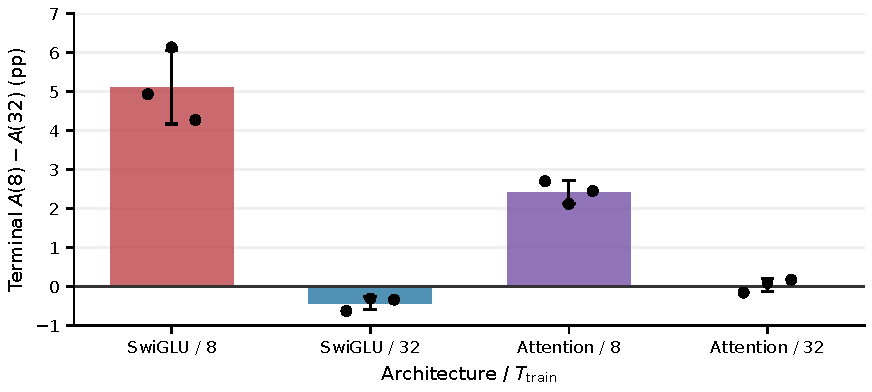
\includegraphics[width=0.85\linewidth]{fig_modern_horizon_drop.pdf}
\caption{\textbf{Matched training removes the strong horizon-extension loss.}
Terminal $A(8)-A(32)$ for the four recursive conditions. Negative values mean
the endpoint improves with additional steps. Points show individual seeds;
bars and error bars show means and sample standard deviations ($n=3$).
This is the difference summary of the curves in \Cref{fig:modern_panel}.}
\label{fig:modern_drop}
\end{figure}

\section{Tiny ImageNet: Readouts and Representation Probes}
\label{app:modern_readouts}

\paragraph{Frozen readout settings.}
Early-window uses $K=8$, adaptive stopping uses norm-ratio threshold 1.5,
and \grace{} uses $(\tau,\alpha)=(1.2,10)$. These settings are not tuned for
attention. Uniform averaging and \grace{} use the available trajectory through
each evaluation horizon. The shared classification head is applied to the
aggregated state, without retraining. The table below retains all attention
readouts, including underperformance of the norm-weighted rule in the matched
32-step condition. The modern experiments support an endpoint-validity
diagnosis rather than universal dominance of \grace{}.

\begin{table}[htbp]
\centering
\caption{\textbf{All frozen attention readouts.} Validation accuracy (\%, mean $\pm$ sample standard deviation, three seeds).}
\label{tab:attention_readouts}
\small
\begin{tabular}{rrrrrrr}
\toprule
$T_{\rm train}$ & $T_{\rm test}$ & Terminal & Early 8 & Uniform & Adaptive & \grace{} \\
\midrule
8 & 8 & $79.62\pm0.08$ & $79.88\pm0.11$ & $79.88\pm0.11$ & $79.40\pm0.20$ & $77.16\pm0.36$ \\
8 & 16 & $78.85\pm0.20$ & $79.88\pm0.11$ & $79.41\pm0.07$ & $79.40\pm0.20$ & $77.16\pm0.36$ \\
8 & 24 & $78.03\pm0.20$ & $79.88\pm0.11$ & $78.92\pm0.21$ & $79.40\pm0.20$ & $77.16\pm0.36$ \\
8 & 32 & $77.20\pm0.33$ & $79.88\pm0.11$ & $78.49\pm0.19$ & $79.40\pm0.20$ & $77.16\pm0.36$ \\
\midrule
32 & 8 & $79.19\pm0.11$ & $78.58\pm0.29$ & $78.58\pm0.29$ & $76.81\pm0.33$ & $57.47\pm3.94$ \\
32 & 16 & $79.36\pm0.19$ & $78.58\pm0.29$ & $79.40\pm0.16$ & $76.81\pm0.33$ & $57.47\pm3.94$ \\
32 & 24 & $79.32\pm0.37$ & $78.58\pm0.29$ & $79.41\pm0.26$ & $76.81\pm0.33$ & $57.47\pm3.94$ \\
32 & 32 & $79.15\pm0.22$ & $78.58\pm0.29$ & $79.41\pm0.24$ & $76.81\pm0.33$ & $57.47\pm3.94$ \\
\bottomrule
\end{tabular}
\end{table}


The horizon headline uses the saved full-trajectory classification results;
the readout table uses the separately classified feature aggregates. Their
attention terminal scores differ by a few examples because BF16 classifier
matrix multiplications use different tensor shapes. Each series is retained
consistently; these small differences do not alter the reported pattern.

\paragraph{Fixed-regularisation representation probes.}
We fit separate RidgeClassifiers with $\alpha_{\rm ridge}=1$ on step-8,
early-eight, and step-32 features, using the same fixed 20,000-example
training subset (subset seed 2026), no feature standardisation, and all
10,000 validation examples. The regularisation is fixed, while each
representation receives its own fitted coefficients. This distinguishes a
loss of linear decodability from failure of the shared trained head alone.

\begin{table}[htbp]
\centering
\caption{\textbf{Fixed-alpha probe accuracy.} Separately fitted probes share ridge $\alpha=1$ and a fixed training subset. Accuracy in percent; loss in pp.}
\label{tab:modern_probes}
\small
\begin{tabular}{lrrrrr}
\toprule
Model & $T_{\rm train}$ & Step 8 & Early 8 & Step 32 & Loss (pp) \\
\midrule
SwiGLU & 8 & $81.31\pm0.14$ & $81.48\pm0.12$ & $79.08\pm0.29$ & $2.23\pm0.17$ \\
SwiGLU & 32 & $81.12\pm0.01$ & $80.75\pm0.06$ & $81.36\pm0.09$ & $-0.24\pm0.08$ \\
Attention & 8 & $79.59\pm0.06$ & $79.79\pm0.07$ & $78.31\pm0.08$ & $1.28\pm0.08$ \\
Attention & 32 & $79.33\pm0.35$ & $79.39\pm0.30$ & $78.98\pm0.30$ & $0.35\pm0.10$ \\
\bottomrule
\end{tabular}
\end{table}


For eight-step training, both architectures lose accuracy under both the
shared head and refitted probes. Matching the training horizon removes the
large probe loss: the SwiGLU probe improves by $0.24\pm0.08$~pp and the
attention probe loses only $0.35\pm0.10$~pp. This is evidence about the tested
linear decoders, not a proof that all task information is irrecoverably lost.

\section{Tiny ImageNet: Robustness and Preliminary Controls}
\label{app:modern_robustness}

\paragraph{Classwise robustness.}
The classwise loss is the mean step-8 accuracy minus mean step-32 accuracy
across seeds, evaluated separately in each of the 200 classes. All classes
are included. SwiGLU has a median loss of 2.67~pp (IQR 0.00--8.67), with
144/200 classes losing accuracy and 124/200 losing at least 2~pp. Attention
has a median loss of 2.00~pp (IQR 0.67--4.00), with 153/200 classes losing
accuracy and 105/200 losing at least 2~pp. The macro-mean losses are 5.11
and 2.42~pp, respectively. The degradation is therefore distributed across
many classes.

\paragraph{Checkpoint sensitivity.}
We evaluate existing saved states without changing the headline selection
rule. Every audited checkpoint has a positive step-8-minus-step-32 loss,
but its magnitude depends on checkpoint age. SwiGLU's selected checkpoints
(epochs 3--4) lose 4.27--6.13~pp, while final-epoch checkpoints lose only
0.59--0.68~pp. Continued eight-step training therefore substantially reduces
the loss even without matched 32-step training. For attention, the top three
saved improving checkpoints per seed lose 2.12--3.49~pp; the selected
checkpoint has the smallest loss among those saved alternatives in each seed.
Intermediate SwiGLU checkpoints and final-epoch attention states were not
retained, limiting the comparisons possible from saved artifacts.

\begin{table}[htbp]
\centering
\caption{\textbf{Checkpoint sensitivity of eight-step-trained models.} Accuracy in percent; loss in pp. Only retained checkpoints are compared.}
\label{tab:checkpoint_sensitivity}
\small
\begin{tabular}{lr l rrrr}
\toprule
Model & Seed & Checkpoint & Epoch & Step 8 & Step 32 & Loss \\
\midrule
SwiGLU & 101 & Selected & 3 & 80.98 & 76.05 & 4.93 \\
SwiGLU & 101 & Final epoch & 30 & 80.71 & 80.12 & 0.59 \\
SwiGLU & 102 & Selected & 4 & 80.82 & 74.69 & 6.13 \\
SwiGLU & 102 & Final epoch & 30 & 80.62 & 79.96 & 0.66 \\
SwiGLU & 103 & Selected & 3 & 80.82 & 76.55 & 4.27 \\
SwiGLU & 103 & Final epoch & 30 & 80.67 & 79.99 & 0.68 \\
Attention & 101 & Selected & 5 & 79.53 & 76.83 & 2.70 \\
Attention & 101 & Saved rank 2 & 4 & 78.91 & 76.08 & 2.83 \\
Attention & 101 & Saved rank 3 & 3 & 78.52 & 75.03 & 3.49 \\
Attention & 102 & Selected & 7 & 79.61 & 77.49 & 2.12 \\
Attention & 102 & Saved rank 2 & 5 & 79.31 & 76.76 & 2.55 \\
Attention & 102 & Saved rank 3 & 4 & 79.27 & 76.28 & 2.99 \\
Attention & 103 & Selected & 5 & 79.72 & 77.27 & 2.45 \\
Attention & 103 & Saved rank 2 & 4 & 79.30 & 76.63 & 2.67 \\
Attention & 103 & Saved rank 3 & 3 & 78.38 & 75.06 & 3.32 \\
\bottomrule
\end{tabular}
\end{table}


\paragraph{Seed-0 gain-sweep pilots.}
Before the paired panel, two SwiGLU pilots used gain values
$\{0.75,1.0,1.1,1.2,1.3,1.4,1.5,1.6\}$. The first trained for eight steps
and evaluated for 32. Its early-minus-terminal gap was already 4.93~pp at
nominal gain, so it failed the predeclared requirement for a competitive
nominal endpoint before gain stress. The aligned 32-step pilot restored the
nominal endpoint but had a maximum early-window advantage of only 0.27~pp,
failing the criterion of at least 1~pp at three consecutive gains. Each pilot
was stopped after seed 0; neither is a three-seed confirmation. These outcomes
motivated the subsequently frozen paired horizon comparison with fresh seeds.
The direct fixed-alpha probe on pooled ConvNeXt features scored 80.52\%.

\begin{table}[htbp]
\centering
\caption{\textbf{Seed-0 SwiGLU pilot readouts at $T_{\rm test}=32$.} Accuracy in percent. Fixed denotes the training-derived global \grace{} profile. Neither pilot continued to further seeds.}
\label{tab:pilot_readouts}
\small
\begin{tabular}{rrrrrrrr}
\toprule
$T_{\rm train}$ & Gain & Terminal & Early 8 & Uniform & Adaptive & \grace{} & Fixed \\
\midrule
8 & 0.75 & 77.72 & 80.76 & 79.71 & 80.34 & 80.70 & 80.36 \\
8 & 1.00 & 75.92 & 80.85 & 78.84 & 80.38 & 80.70 & 80.39 \\
8 & 1.10 & 75.09 & 80.89 & 78.52 & 80.35 & 80.69 & 80.56 \\
8 & 1.20 & 74.47 & 80.78 & 78.31 & 80.36 & 80.72 & 80.59 \\
8 & 1.30 & 73.77 & 80.82 & 77.92 & 80.32 & 80.68 & 80.68 \\
8 & 1.40 & 73.08 & 80.87 & 77.65 & 80.28 & 80.71 & 80.78 \\
8 & 1.50 & 72.44 & 80.83 & 77.41 & 80.37 & 80.69 & 80.80 \\
8 & 1.60 & 71.86 & 80.82 & 77.13 & 80.29 & 80.76 & 80.81 \\
\midrule
32 & 0.75 & 80.77 & 79.25 & 80.63 & 80.77 & 80.50 & 80.06 \\
32 & 1.00 & 80.75 & 79.72 & 80.85 & 80.71 & 80.64 & 80.33 \\
32 & 1.10 & 80.62 & 79.77 & 80.78 & 80.64 & 80.52 & 80.33 \\
32 & 1.20 & 80.54 & 79.84 & 80.77 & 80.59 & 80.54 & 80.39 \\
32 & 1.30 & 80.33 & 79.95 & 80.71 & 80.57 & 80.59 & 80.40 \\
32 & 1.40 & 80.15 & 80.07 & 80.80 & 80.43 & 80.63 & 80.51 \\
32 & 1.50 & 80.15 & 80.15 & 80.77 & 80.57 & 80.67 & 80.70 \\
32 & 1.60 & 79.93 & 80.20 & 80.79 & 80.49 & 80.66 & 80.68 \\
\bottomrule
\end{tabular}
\end{table}


The pilots also compare per-sample \grace{} with a fixed temporal profile,
formed by averaging normalised training-sample \grace{} weights at gain 1.3
and then freezing that profile across gains. They show no consistent advantage
for per-sample weighting. At gain 1.6 in the aligned pilot, uniform averaging,
\grace{}, and the fixed profile score 80.79\%, 80.66\%, and 80.68\%,
respectively. A saved-trajectory horizon audit of the eight-step pilot at gain
1 gives terminal accuracy 80.82\% at step 8 and 75.92\% at step 32, consistent
with the later paired panel. No new canonical-DEQ experiment was completed;
the DEQ-style evidence in \Cref{app:deq} remains the original limited check.

\section{Tiny ImageNet: Model Scale, Runtime, and Memory}
\label{app:modern_cost}

\begin{table}[htbp]
\centering
\caption{\textbf{Scale of the modern recursive systems.} The executed frozen
backbone has 27,820,128 parameters. One multiply-add counts as two FLOPs.}
\label{tab:modern_scale}
\small
\begin{tabular}{lrr}
\toprule
Quantity & SwiGLU & Attention \\
\midrule
Input & pooled 768-d & $49\times768$ tokens \\
Recursive width & 512 & 256 \\
Intermediate width & 2,048 & 1,024 \\
Attention heads & --- & 8 \\
Trainable head parameters & 3,648,712 & 1,301,960 \\
Executed total parameters & 31,468,840 & 29,122,088 \\
Dominant recurrent FLOPs/step & 6,291,456 & 107,517,600 \\
\bottomrule
\end{tabular}
\end{table}

For state width $d$, intermediate width $m$, $n$ tokens, and $h$ attention
heads, recurrent FLOPs are counted as $6dm$ for SwiGLU and
$8nd^2+4n^2d+5hn^2+6ndm$ for attention ($n=50$ including the class token).
These counts exclude the frozen backbone, one-time input projection, final
classifier, LayerNorm, and lower-order elementwise operations.

\paragraph{Readout benchmark.}
The measurements in \Cref{tab:cost_main} use the first seed-0 SwiGLU pilot,
independently of its scientific continuation outcome. Settings are BF16,
batch 512, $d=512$, $T=32$, gain 1.3, and early window 8, on an RTX 5080
Laptop GPU. CUDA events measure elapsed device time after 10 warm-ups,
with the median of 25 timed repetitions reported. Full recurrent-head
inference starts with cached backbone features and includes recursion and
classification; it excludes image loading and backbone execution. Additional
peak allocated memory is measured relative to the warmed-up baseline for
each repetition and summarised by its median. It excludes baseline model,
input, and cached-tensor allocations and is not CUDA reserved or total process
memory. Readout-only measurements start with an already allocated trajectory.

\begin{table}[htbp]
\centering
\caption{\textbf{Full recurrent-head and readout-only benchmark.} Latencies in ms and additional peak allocations in MiB; the precomputed trajectory is part of the baseline in readout-only measurements.}
\label{tab:cost_detail}
\small
\begin{tabular}{lrrrr}
\toprule
Readout & Full ms & Readout ms & Full MiB & Readout MiB \\
\midrule
Terminal & 6.727 & 0.113 & 8.00 & 2.00 \\
Early window & 1.803 & 0.135 & 11.50 & 2.50 \\
Adaptive & 13.840 & 0.208 & 9.01 & 2.52 \\
Uniform streaming & 6.889 & 0.117 & 8.50 & 2.50 \\
\grace{}, stored & 6.948 & 0.317 & 48.56 & 32.06 \\
\grace{}, streaming & 9.681 & 3.653 & 8.51 & 3.01 \\
\bottomrule
\end{tabular}
\end{table}


\begin{table}[htbp]
\centering
\caption{\textbf{Readout complexity per example.} Arithmetic excludes the
recurrent update and classifier. $t\leq T$ is the adaptive stopping step.}
\label{tab:readout_complexity}
\small
\begin{tabular}{lccc}
\toprule
Readout & Arithmetic & State storage & Halts recurrence \\
\midrule
Terminal & $O(d)$ & $O(d)$ & No \\
Early window & $O(Kd)$ & $O(d)$ & At $K$ \\
Adaptive & $O(td)$ & $O(d)$ & Yes \\
Uniform streaming & $O(Td)$ & $O(d)$ & No \\
\grace{}, stored & $O(Td)$ & $O(Td)$ & No \\
\grace{}, streaming & $O(Td)$ & $O(d)$ & No \\
\bottomrule
\end{tabular}
\end{table}

Streaming \grace{} maintains a weighted numerator and denominator while
discarding each state after use. This explains its memory benefit without
implying a speedup: the measured eager loop costs 9.68~ms versus 6.95~ms
for stored-trajectory \grace{}. Adaptive active-set compaction costs 13.84~ms
for this dense batch. These are implementation- and hardware-specific
measurements, not architecture-independent latency guarantees.

\paragraph{Training and evaluation allocations.}
The attention training runs separately record absolute CUDA allocator peaks.
For eight-step training, allocated/reserved peaks are 871.56/1,100~MiB;
for 32-step training they are 3,054.91/3,594~MiB. Evaluation peaks are
219.53/298~MiB in both conditions. The peaks are identical across the three
seeds within each condition. Completed training wall times are
499.42/498.15/505.00~s for eight steps and
1,582.40/1,635.76/2,312.70~s for 32 steps. These absolute allocator peaks
measure a different quantity from the additional-memory benchmark above.

\paragraph{Execution provenance.}
Protocols, configurations, seeds, and checkpoint selection were frozen for
each experiment before its results. The final panel contains 12 completed
scientific runs, plus the two separate seed-0 pilots. Two interrupted
32-step attention attempts were retained and restarted from the same frozen
seed/configuration because optimizer and RNG states were unavailable for an
exact resume; they are not extra scientific replicates. Scientific artifacts
retain SHA-256 configuration and checkpoint records. The robustness analyses
use existing checkpoints, with no post-result changes to architectures,
gains, readout thresholds, probe regularisation, or the headline selection rule.


\section{Extended Related Work}
\label{app:related}

\paragraph{Reservoir computing and the echo state property.}
Echo state networks~\citep{jaeger2001echo} and liquid state
machines~\citep{maass2002real} established the reservoir computing paradigm.
The echo state property (ESP), the requirement that reservoir states be
uniquely determined by input history, is traditionally ensured by
constraining $\sr < 1$, though this condition is neither necessary nor
sufficient~\citep{yildiz2012revisiting}. Our work characterises what happens
when $\sr$ is intentionally pushed past the ESP boundary: the substrate
remains useful, but only within a temporal window formalised as the prefix
grace period.

\paragraph{Edge of chaos and criticality.}
Bertschinger and Natschl\"ager~\citep{bertschinger2004real} showed that
reservoir computation is optimised at the critical boundary $\sr \approx 1$.
Subsequent work formalised memory-nonlinearity trade-offs at
criticality~\citep{dambre2012information}. In nearby deep-network mean-field
analyses, transient chaos and signal propagation likewise sharpen at the
ordered/chaotic boundary~\citep{poole2016exponential,schoenholz2017deep}.
Our regime lies beyond this boundary, showing that useful computation
persists in the supercritical phase provided one reads out from the right
portion of the trajectory.

\paragraph{Non-normal amplification.}
Trefethen and Embree~\citep{trefethen2005spectra} established that non-normal
matrices exhibit transient growth even when spectral radius predicts
asymptotic stability. Hennequin et al.~\citep{hennequin2012nonnormal}
separate non-normal amplification from near-critical slowing in balanced
networks. Recent nnRNN work likewise uses Schur-structured non-normal
connectivity and shows that training preserves or suppresses transient
structure according to task demand~\citep{kerg2019nonnormal}. Our norm-ratio
criterion (\Cref{eq:growth}) directly measures this amplification and uses it
as a readout signal.

\paragraph{Physical neuromorphic substrates.}
Recent physical neural-network and photonic-scattering systems show that
dynamical media, wave propagation, and hardware readout can serve as
trainable computational resources~\citep{momeni2025training,
wanjura2025fully,wang2024large}. These settings make readout timing
especially salient because the measured state and sampling time are part of
the physical computation, not merely an implementation detail.

\paragraph{Vanishing and exploding gradients.}
The classical gradient pathology in RNNs~\citep{pascanu2013difficulty,
bengio1994learning} motivates architectural solutions (LSTMs, GRUs,
unitary RNNs~\citep{arjovsky2016unitary}). These address training stability;
our work addresses inference-time readout. Gradient clipping stabilises
learning; trajectory-aware readouts stabilise decoding in the regimes studied.

\paragraph{Edge of stability in optimisation.}
Cohen et al.~\citep{cohen2021gradient} identify an ``edge of stability'' in
gradient descent where the Hessian's largest eigenvalue hovers near $2/\eta$.
Our phenomenon is distinct: it concerns readout timing of a fixed dynamical
substrate, not optimiser dynamics.

\paragraph{Deep equilibrium and neural ODE models.}
DEQ models~\citep{bai2019deep} and neural ODEs~\citep{chen2018neural} are
the purest instantiations of the endpoint assumption. Near bifurcation
boundaries, trajectory-level readout could improve robustness. Consistency
DEQs cast DEQ inference as movement along a fixed ODE trajectory and train
intermediate states to map directly to the equilibrium
\citep{lin2026consistency}. Our setting asks a different question: whether the
endpoint remains the best object of inference at all. \grace{} is therefore a
training-free trajectory-weighted diagnostic rather than a distillation method
for predicting the fixed point.

\paragraph{Adaptive computation, early exit, and overthinking.}
Adaptive Computation Time and PonderNet learn how many recurrent steps to use
for each input~\citep{graves2016adaptive,banino2021pondernet}.
Early-exit systems and overthinking analyses show that intermediate
predictions can outperform deeper computations~\citep{teerapittayanon2016branchynet,
kaya2019shallow,elhoushi2024layerskip}. Our setting differs in both axis and
failure mode: the intermediate object is a time-indexed dynamical state rather
than a shallower network layer or a learned halting distribution, and the issue
is not only saving computation but detecting when extra computation destroys
endpoint validity while a usable prefix remains.

\paragraph{Deep reservoir computing.}
Gallicchio and Micheli~\citep{gallicchio2017echo} show that global spectral
radius increases monotonically with reservoir depth, linking architectural
depth to shrinking stability margins. Our result is complementary: once a
system is driven past those margins, decoder choice determines whether the
remaining transient computation is still recoverable.



\section{Proofs}
\label{app:proofs}

\subsection{Proof of Proposition~\ref{prop:grace}}

\begin{proof}
Let $\bar r_t$ be the reference norm-ratio curve from the proposition. By assumption,
\[
  \bar r_t \geq \bar r_{t_0}\,\kappa^{t-t_0}
  \qquad \text{for all } t \geq t_0.
\]
If
\[
  t \geq t_0 + \left\lceil
  \frac{\log(R_{\max}/\bar r_{t_0})}{\log\kappa}
  \right\rceil + 1,
\]
then
$t - t_0 > \log(R_{\max}/\bar r_{t_0})/\log\kappa$, and therefore
\[
  \bar r_t \geq \bar r_{t_0}\,\kappa^{t-t_0} > R_{\max}.
\]
Hence $\operatorname{acc}(\phi_t) < \alpha$ for all such $t$. It follows that
the grace-period definition cannot certify any prefix extending beyond
\[
  t_0 + \left\lceil
  \frac{\log(R_{\max}/\bar r_{t_0})}{\log\kappa}
  \right\rceil,
\]
which is exactly the claimed upper bound on $G(\sr,\alpha)$.
\end{proof}

\subsection{Proposition A1: Prefix-Limit Behaviour of \grace{}}
\label{app:prop:prefix}

\begin{proposition}[Prefix-limit behaviour]
\label{prop:prefix_limit}
Let $w_t(\alpha, \tau) \propto \exp(-\alpha\max(0, g_t - \tau))$. If
the threshold crossing is unique, i.e., there exists $t^\star\geq1$ such that
$g_t \leq \tau$ for $t \leq t^\star$ and $g_t > \tau$ for $t > t^\star$,
then as $\alpha \to \infty$,
\[
  w_t \to \begin{cases} 1 / t^\star, & t \leq t^\star, \\ 0, & t > t^\star. \end{cases}
\]
\end{proposition}

\begin{proof}
For $t \leq t^\star$, $\tilde{w}_t = 1$. For $t > t^\star$,
$\tilde{w}_t = \exp(-\alpha(g_t - \tau)) \to 0$ as $\alpha \to \infty$
because $g_t - \tau > 0$. Normalising over the $t^\star$ surviving
weights gives $w_t = 1/t^\star$ for $t \leq t^\star$.
\end{proof}

This result connects \grace{} to prefix selection: in the large-$\alpha$
limit, \grace{} places uniform mass on the largest contiguous
norm-threshold prefix and zero mass beyond it. The prefix is not assumed to
equal the accuracy-defined grace period in Definition~\ref{def:grace_period};
empirically, the norm-threshold prefix acts as a conservative proxy. Thus
\grace{} interpolates continuously between uniform averaging ($\alpha = 0$)
and hard norm-threshold prefix selection ($\alpha \to \infty$).

\subsection{Lemma A2: Tail Suppression Preserves Separability}
\label{app:lemma:tail}

\begin{lemma}[Tail suppression preserves separability under bounded prefix distortion]
\label{lemma:tail}
Let $(\bx_i,y_i)_{i=1}^N$ be labelled examples with $y_i \in \{-1,+1\}$.
For each timestep $t = 1,\ldots,T$, write the observed feature as
$\mathbf{h}_t^{(i)} = \mathbf{s}_t^{(i)} + \mathbf{e}_t^{(i)}$.
Assume there exist a prefix length $G$, a separator $(\mathbf{w}, b)$, and a
margin $\gamma > 0$ such that
\[
  y_i\bigl(\mathbf{w}^{\top}\mathbf{s}_t^{(i)} + b\bigr) \geq \gamma
  \qquad \text{for all } i \text{ and all } t \leq G.
\]
Assume also that for $t \leq G$ the distortion obeys
$\|\mathbf{e}_t^{(i)}\| \leq \eta_t$ for all $i$. Let nonnegative,
sample-dependent weights $(\lambda_t^{(i)})_{t=1}^T$ satisfy
$\sum_{t=1}^T \lambda_t^{(i)} = 1$, $\lambda_t^{(i)} = 0$ for $t > G$, and
\[
  \|\mathbf{w}\| \sup_i \sum_{t=1}^G \lambda_t^{(i)} \eta_t < \gamma.
\]
Then the aggregated feature
\[
  \bar{\mathbf{h}}^{(i)} = \sum_{t=1}^T \lambda_t^{(i)} \mathbf{h}_t^{(i)}
\]
is linearly separable by the same separator $(\mathbf{w}, b)$, with margin at
least
\[
  \gamma - \|\mathbf{w}\|\sup_i \sum_{t=1}^G \lambda_t^{(i)} \eta_t > 0.
\]
\end{lemma}

\begin{proof}
Since $\lambda_t^{(i)} = 0$ for $t > G$ and
$\sum_{t=1}^T \lambda_t^{(i)} = 1$,
\begin{align*}
  y_i\bigl(\mathbf{w}^{\top}\bar{\mathbf{h}}^{(i)} + b\bigr)
  &= y_i\left(
  \mathbf{w}^{\top}\sum_{t=1}^G \lambda_t^{(i)}
  \bigl(\mathbf{s}_t^{(i)} + \mathbf{e}_t^{(i)}\bigr) + b
  \right) \\
  &= \sum_{t=1}^G \lambda_t^{(i)}\,
  y_i\bigl(\mathbf{w}^{\top}\mathbf{s}_t^{(i)} + b\bigr)
  + y_i\,\mathbf{w}^{\top}\sum_{t=1}^G \lambda_t^{(i)} \mathbf{e}_t^{(i)} \\
  &\geq \sum_{t=1}^G \lambda_t^{(i)} \gamma
  - \|\mathbf{w}\| \sum_{t=1}^G \lambda_t^{(i)} \|\mathbf{e}_t^{(i)}\| \\
  &\geq \gamma - \|\mathbf{w}\| \sum_{t=1}^G \lambda_t^{(i)} \eta_t \\
  &\geq \gamma - \|\mathbf{w}\|\sup_j \sum_{t=1}^G \lambda_t^{(j)} \eta_t \\
  &> 0.
\end{align*}
Thus every aggregated feature is correctly classified by the same separator,
with the stated margin.
\end{proof}

This lemma captures the role of tail suppression in the mechanism argument:
if a prefix is separable and accumulated prefix distortion stays below the
available margin, then any per-sample convex readout that excludes the tail
preserves separability. \grace{} approximates this behaviour by
down-weighting high-growth late timesteps. The statement is written in binary
margin form; the multiclass analogue follows by applying the same bound to
each pairwise score gap of a linear head.

\subsection{Scaled-Kreiss Refinement for Smooth Activations}
\label{app:kreiss_refinement}

The main text uses Proposition~\ref{prop:grace} because it applies directly to
the measured norm-ratio proxy. This appendix upgrades that proposition in
operator terms. There, the conditional factor $\kappa$ plays the role of a
post-$t_0$ amplification rate; here, that rate is decomposed into a radial term
and an envelope factor, first through a frozen scaled-Kreiss constant and then
through a full Jacobian cocycle. The resulting corollaries replace the
norm-threshold assumption of Proposition~\ref{prop:grace} with a
margin-vs.-remainder criterion. The tanh remainder bound below applies
directly to the bounded-activation ESN branch of our taxonomy; the modReLU and
LeakyReLU cases admit analogous activation-specific remainder bounds, but we do
not state them here.

For smooth activations, one can refine the main-text mechanism locally by
separating linearised amplification from nonlinear remainder. The first step is
a forced linear bound controlled by the scaled Kreiss constant of a frozen
effective operator; the final theorem below then replaces that frozen operator
by a trajectory-dependent Jacobian cocycle. Unless stated otherwise, norms in
this subsection are Euclidean/operator spectral norms.

\begin{lemma}[Scaled-Kreiss envelope for forced linear dynamics]
\label{lemma:scaled_kreiss}
Let $\mathbf{A} \in \C^{d \times d}$ with $\rho_\ast = \rho(\mathbf{A}) > 0$, and define
the scaled Kreiss constant
\begin{equation}
  K_{\rho_\ast}(\mathbf{A})
  := \sup_{|z| > \rho_\ast} (|z| - \rho_\ast)\,\|(z\mathbf{I} - \mathbf{A})^{-1}\|
  = K(\mathbf{A}/\rho_\ast).
\end{equation}
Assume $K_{\rho_\ast}(\mathbf{A})<\infty$.
Consider the forced linear recurrence
\[
  \boldsymbol{\delta}_{t+1} = \mathbf{A} \boldsymbol{\delta}_t + \mathbf{q}_t,
  \qquad \boldsymbol{\delta}_0 = \mathbf{0}.
\]
Then for every $t \geq 1$,
\begin{equation}
  \|\boldsymbol{\delta}_t\|
  \leq e d\,K_{\rho_\ast}(\mathbf{A})
  \sum_{s=0}^{t-1} \rho_\ast^{\,t-1-s}\,\|\mathbf{q}_s\|.
  \label{eq:scaled_kreiss_forced}
\end{equation}
\end{lemma}

\begin{proof}
Let $\mathbf{B} = \mathbf{A}/\rho_\ast$. By variation of constants,
\[
  \boldsymbol{\delta}_t
  = \sum_{s=0}^{t-1} \mathbf{A}^{t-1-s} \mathbf{q}_s
  = \sum_{s=0}^{t-1} \rho_\ast^{\,t-1-s}\,\mathbf{B}^{t-1-s}\mathbf{q}_s.
\]
The discrete Kreiss matrix theorem gives
\[
  \sup_{k \geq 0}\|\mathbf{B}^k\| \leq e d\,K(\mathbf{B})
  = e d\,K_{\rho_\ast}(\mathbf{A})
\]
\citep{trefethen2005spectra}. Therefore
\[
  \|\mathbf{A}^k\|
  = \rho_\ast^k \|\mathbf{B}^k\|
  \leq e d\,K_{\rho_\ast}(\mathbf{A})\,\rho_\ast^k.
\]
Substituting this into the variation-of-constants formula yields
\Cref{eq:scaled_kreiss_forced}.
\end{proof}

For smooth activations the one-step nonlinear remainder is quadratic in the
distance from the linearisation point. For tanh this yields an explicit
constant.

\begin{lemma}[tanh linearisation remainder]
\label{lemma:tanh_remainder}
Fix an input $\bx\in\R^n$ and real-valued parameters
$\bW\in\R^{d\times d}$, $\bU\in\R^{d\times n}$, and $\mathbf{b}\in\R^d$.
Define
\[
  F_{\bx}(\bz) = \tanh(\bW\bz + \bU\bx + \mathbf{b}),
\]
with tanh applied componentwise. Let
\[
  J_{\bx}(\bar{\bz})
  = D\tanh(\bW\bar{\bz} + \bU\bx + \mathbf{b})\,\bW.
\]
Then for all $\bz,\bar{\bz} \in \R^d$,
\begin{equation}
  \|F_{\bx}(\bz) - F_{\bx}(\bar{\bz})
  - J_{\bx}(\bar{\bz})(\bz - \bar{\bz})\|
  \leq \frac{L_{\tanh}}{2}\,\|\bW\|^2\,\|\bz - \bar{\bz}\|^2,
  \label{eq:tanh_remainder}
\end{equation}
where
\[
  L_{\tanh}
  := \sup_{u \in \R} |\tanh''(u)|
  = \frac{4}{3\sqrt{3}}.
\]
\end{lemma}

\begin{proof}
Write $\mathbf{a}(\bz) = \bW\bz + \bU\bx + \mathbf{b}$. Since tanh acts
componentwise,
\[
  J_{\bx}(\bz) = D\tanh(\mathbf{a}(\bz))\,\bW.
\]
For any $\bz,\bar{\bz}$, the operator norm of the diagonal difference obeys
\begin{align*}
  \|D\tanh(\mathbf{a}(\bz)) - D\tanh(\mathbf{a}(\bar{\bz}))\|
  &\leq \max_j |\tanh'(a_j(\bz)) - \tanh'(a_j(\bar{\bz}))| \\
  &\leq L_{\tanh}\,\|\mathbf{a}(\bz) - \mathbf{a}(\bar{\bz})\|_\infty \\
  &\leq L_{\tanh}\,\|\bW\|\,\|\bz - \bar{\bz}\|.
\end{align*}
Multiplying by $\|\bW\|$ gives the Jacobian Lipschitz bound
\[
  \|J_{\bx}(\bz) - J_{\bx}(\bar{\bz})\|
  \leq L_{\tanh}\,\|\bW\|^2\,\|\bz - \bar{\bz}\|.
\]
The integral remainder formula then yields
\begin{align*}
  &\|F_{\bx}(\bz) - F_{\bx}(\bar{\bz})
  - J_{\bx}(\bar{\bz})(\bz - \bar{\bz})\| \\
  &\qquad\leq \int_0^1
  \|J_{\bx}(\bar{\bz} + \theta(\bz-\bar{\bz})) - J_{\bx}(\bar{\bz})\|
  \,\|\bz-\bar{\bz}\|\,d\theta \\
  &\qquad\leq \int_0^1
  \theta\,L_{\tanh}\,\|\bW\|^2\,\|\bz-\bar{\bz}\|^2\,d\theta
  = \frac{L_{\tanh}}{2}\,\|\bW\|^2\,\|\bz-\bar{\bz}\|^2.
\end{align*}
\end{proof}

The previous two lemmas combine into a simple margin-vs.-remainder criterion
for any frozen linearisation.

\begin{proposition}[Frozen-linear margin criterion]
\label{prop:margin_remainder}
Let $(\bx_i,y_i)_{i=1}^N$ with $y_i \in \{-1,+1\}$, and suppose that at a fixed
timestep $t$ the true features admit a decomposition
\[
  \bz_t^{(i)} = \tilde{\bz}_t^{(i)} + \mathbf{e}_t^{(i)}.
\]
Assume there exists a separator $(\mathbf{w}_t, b_t)$ and a margin $m_t > 0$
such that
\[
  y_i\bigl(\mathbf{w}_t^\top \tilde{\bz}_t^{(i)} + b_t\bigr) \geq m_t
  \qquad \text{for all } i.
\]
If
\[
  \max_i \|\mathbf{e}_t^{(i)}\| < \frac{m_t}{\|\mathbf{w}_t\|},
\]
then the same separator classifies the true features correctly, with margin at
least
\[
  m_t - \|\mathbf{w}_t\|\max_i \|\mathbf{e}_t^{(i)}\| > 0.
\]

Moreover, as an idealized autonomous/frozen-linearisation case, suppose the
remainders satisfy a frozen linear recurrence
\[
  \mathbf{e}_{s+1}^{(i)} = J_\ast \mathbf{e}_s^{(i)} + \mathbf{r}_s^{(i)},
  \qquad \mathbf{e}_0^{(i)} = \mathbf{0},
\]
for some fixed operator $J_\ast \in \R^{d \times d}$ with
$\rho_\ast = \rho(J_\ast) > 0$, and assume
$\|\mathbf{r}_s^{(i)}\| \leq R_s$ for all $i,s$. Then
\begin{equation}
  \max_i \|\mathbf{e}_t^{(i)}\|
  \leq e d\,K_{\rho_\ast}(J_\ast)
  \sum_{s=0}^{t-1} \rho_\ast^{\,t-1-s} R_s.
  \label{eq:margin_remainder_generic}
\end{equation}
In this idealized case, if $J_\ast$ is the local Jacobian used in the
linearisation and each $\mathbf{r}_s^{(i)}$ is the corresponding one-step
Taylor remainder at a reference point $\bar{\bz}_s^{(i)}$, then
Lemma~\ref{lemma:tanh_remainder} gives
\[
  R_s \leq \frac{L_{\tanh}}{2}\,\|\bW\|^2 D_s^2,
  \qquad
  D_s := \max_i \|\bz_s^{(i)} - \bar{\bz}_s^{(i)}\|.
\]
Hence timestep $t$ remains separable whenever
\begin{equation}
  \frac{L_{\tanh}}{2}\,\|\bW\|^2\,e d\,K_{\rho_\ast}(J_\ast)
  \sum_{s=0}^{t-1} \rho_\ast^{\,t-1-s} D_s^2
  < \frac{m_t}{\|\mathbf{w}_t\|}.
  \label{eq:tanh_margin_condition}
\end{equation}
\end{proposition}

\begin{proof}
For the first claim,
\begin{align*}
  y_i\bigl(\mathbf{w}_t^\top \bz_t^{(i)} + b_t\bigr)
  &= y_i\bigl(\mathbf{w}_t^\top \tilde{\bz}_t^{(i)} + b_t\bigr)
   + y_i\,\mathbf{w}_t^\top \mathbf{e}_t^{(i)} \\
  &\geq m_t - \|\mathbf{w}_t\|\,\|\mathbf{e}_t^{(i)}\| \\
  &\geq m_t - \|\mathbf{w}_t\| \max_j \|\mathbf{e}_t^{(j)}\| \\
  &> 0.
\end{align*}
Thus the same separator still classifies the true features, with the stated
margin.

For the bound \Cref{eq:margin_remainder_generic}, apply
Lemma~\ref{lemma:scaled_kreiss} to the recurrence for each $i$ and then take
the maximum over $i$. The tanh specialisation follows by substituting the
Taylor bound from Lemma~\ref{lemma:tanh_remainder}. The final separability
criterion is then exactly the first claim applied with the resulting upper
bound on $\max_i\|\mathbf{e}_t^{(i)}\|$.
\end{proof}

The frozen operator above is a convenient expository model. The rigorous
trajectory-dependent treatment is the nonautonomous Jacobian-cocycle argument
below, where the local Jacobian may vary with both sample and timestep.

\begin{theorem}[Trajectory-dependent margin criterion]
\label{thm:trajectory_margin}
Fix real-valued tanh dynamics
\[
  F_{\bx}(\bz) = \tanh(\bW\bz + \bU\bx + \mathbf{b}).
\]
For each sample $i$, let $(\bar{\bz}_s^{(i)})_{s=0}^t$ be a reference path and define
\[
  J_s^{(i)}
  := D\tanh(\bW\bar{\bz}_s^{(i)} + \bU\bx_i + \mathbf{b})\,\bW,
\]
and the Jacobian cocycle
\[
  \Phi_{t:s}^{(i)}
  :=
  \begin{cases}
    J_{t-1}^{(i)} \cdots J_s^{(i)}, & s < t,\\
    \mathbf{I}, & s=t.
  \end{cases}
\]
Let the true trajectory satisfy
\[
  \bz_{s+1}^{(i)} = F_{\bx_i}(\bz_s^{(i)}),
\]
and let the linearised surrogate start from the same initial condition
$\tilde{\bz}_0^{(i)} = \bz_0^{(i)}$ and evolve by
\[
  \tilde{\bz}_{s+1}^{(i)}
  = F_{\bx_i}(\bar{\bz}_s^{(i)})
    + J_s^{(i)}(\tilde{\bz}_s^{(i)} - \bar{\bz}_s^{(i)}).
\]
Assume there exist deterministic numbers $M_{t,s}$ such that
\[
  \max_i \|\Phi_{t:s}^{(i)}\| \leq M_{t,s}
  \qquad \text{for all } 0 \leq s \leq t.
\]
If the surrogate features at time $t$ admit a separator $(\mathbf{w}_t,b_t)$
with margin $m_t > 0$,
\[
  y_i\bigl(\mathbf{w}_t^\top \tilde{\bz}_t^{(i)} + b_t\bigr) \geq m_t
  \qquad \text{for all } i,
\]
then the true features are correctly classified whenever
\begin{equation}
  \frac{L_{\tanh}}{2}\,\|\bW\|^2
  \sum_{s=0}^{t-1} M_{t,s+1} D_s^2
  < \frac{m_t}{\|\mathbf{w}_t\|},
  \qquad
  D_s := \max_i \|\bz_s^{(i)} - \bar{\bz}_s^{(i)}\|.
  \label{eq:trajectory_margin_condition}
\end{equation}
In particular, if there exist $\rho_\ast > 0$ and $C_t$ such that
\[
  M_{t,s+1} \leq C_t\,\rho_\ast^{\,t-1-s}
  \qquad \text{for all } s < t,
\]
then the sufficient condition
\begin{equation}
  \frac{L_{\tanh}}{2}\,\|\bW\|^2\,C_t
  \sum_{s=0}^{t-1} \rho_\ast^{\,t-1-s} D_s^2
  < \frac{m_t}{\|\mathbf{w}_t\|},
  \label{eq:trajectory_margin_geometric}
\end{equation}
also guarantees separability of the true timestep-$t$ features.
\end{theorem}

\begin{proof}
Let $\mathbf{e}_s^{(i)} = \bz_s^{(i)} - \tilde{\bz}_s^{(i)}$. Subtracting the
surrogate recurrence from the true recurrence gives
\[
  \mathbf{e}_{s+1}^{(i)}
  = J_s^{(i)} \mathbf{e}_s^{(i)} + \mathbf{r}_s^{(i)},
\]
where
\[
  \mathbf{r}_s^{(i)}
  := F_{\bx_i}(\bz_s^{(i)}) - F_{\bx_i}(\bar{\bz}_s^{(i)})
   - J_s^{(i)}(\bz_s^{(i)} - \bar{\bz}_s^{(i)}).
\]
By Lemma~\ref{lemma:tanh_remainder},
\[
  \|\mathbf{r}_s^{(i)}\|
  \leq \frac{L_{\tanh}}{2}\,\|\bW\|^2\,
  \|\bz_s^{(i)} - \bar{\bz}_s^{(i)}\|^2
  \leq \frac{L_{\tanh}}{2}\,\|\bW\|^2 D_s^2.
\]
The variation-of-constants formula for time-varying linear recurrences yields
\[
  \mathbf{e}_t^{(i)}
  = \sum_{s=0}^{t-1} \Phi_{t:s+1}^{(i)} \mathbf{r}_s^{(i)}.
\]
Therefore
\[
  \max_i \|\mathbf{e}_t^{(i)}\|
  \leq \frac{L_{\tanh}}{2}\,\|\bW\|^2
  \sum_{s=0}^{t-1} M_{t,s+1} D_s^2.
\]
If \Cref{eq:trajectory_margin_condition} holds, then
$\max_i \|\mathbf{e}_t^{(i)}\| < m_t/\|\mathbf{w}_t\|$, so
Proposition~\ref{prop:margin_remainder} implies that the same separator
correctly classifies the true features. The geometric specialisation
\Cref{eq:trajectory_margin_geometric} follows immediately from the bound
$M_{t,s+1} \leq C_t\rho_\ast^{\,t-1-s}$.
\end{proof}

The remaining step is to package the cocycle envelope into a single
finite-horizon quantity.

\begin{definition}[Finite-horizon cocycle envelope]
\label{def:cocycle_envelope}
Under the hypotheses of \Cref{thm:trajectory_margin}, fix $\lambda > 0$ and define
\begin{equation}
  \mathcal{R}_t(\lambda)
  := \max_i \sup_{(\mathbf{q}_0,\dots,\mathbf{q}_{t-1}) \not\equiv \mathbf{0}}
  \frac{\left\|\sum_{s=0}^{t-1}\Phi_{t:s+1}^{(i)} \mathbf{q}_s\right\|}
       {\sum_{s=0}^{t-1}\lambda^{\,t-1-s}\|\mathbf{q}_s\|}.
  \label{eq:cocycle_envelope}
\end{equation}
\end{definition}

This is a weighted input-output norm of the nonautonomous linearised system,
and serves as the finite-horizon analogue of the frozen scaled-Kreiss constant.

\begin{lemma}[Cocycle envelope controls Jacobian products]
\label{lemma:cocycle_envelope}
For every $0 \leq s < t$,
\begin{equation}
  \max_i \|\Phi_{t:s+1}^{(i)}\|
  \leq \mathcal{R}_t(\lambda)\,\lambda^{\,t-1-s}.
  \label{eq:cocycle_envelope_phi}
\end{equation}
Moreover, in the autonomous frozen case $J_u^{(i)} \equiv J_\ast$ for all
$i,u$, with $\rho_\ast = \rho(J_\ast)$, one has
\begin{equation}
  \mathcal{R}_t(\rho_\ast)
  \leq e d\,K_{\rho_\ast}(J_\ast).
  \label{eq:cocycle_envelope_kreiss}
\end{equation}
\end{lemma}

\begin{proof}
For \Cref{eq:cocycle_envelope_phi}, fix $s<t$, an index $i$, and a vector
$\mathbf{v}\neq \mathbf{0}$. In \Cref{eq:cocycle_envelope}, choose
$\mathbf{q}_u=\mathbf{0}$ for $u\neq s$ and $\mathbf{q}_s=\mathbf{v}$. Then
\[
  \frac{\|\Phi_{t:s+1}^{(i)}\mathbf{v}\|}
       {\lambda^{\,t-1-s}\|\mathbf{v}\|}
  \leq \mathcal{R}_t(\lambda).
\]
Taking the supremum over $\mathbf{v}\neq \mathbf{0}$ and then the maximum over
$i$ proves \Cref{eq:cocycle_envelope_phi}.

For \Cref{eq:cocycle_envelope_kreiss}, the output of the frozen linear system
\[
  \boldsymbol{\delta}_{u+1} = J_\ast \boldsymbol{\delta}_u + \mathbf{q}_u,
  \qquad \boldsymbol{\delta}_0 = \mathbf{0},
\]
at time $t$ is
\[
  \boldsymbol{\delta}_t = \sum_{s=0}^{t-1} J_\ast^{\,t-1-s}\mathbf{q}_s.
\]
Lemma~\ref{lemma:scaled_kreiss} yields
\[
  \|\boldsymbol{\delta}_t\|
  \leq e d\,K_{\rho_\ast}(J_\ast)
  \sum_{s=0}^{t-1}\rho_\ast^{\,t-1-s}\|\mathbf{q}_s\|.
\]
Taking the supremum over all nonzero forcing sequences gives
\Cref{eq:cocycle_envelope_kreiss}.
\end{proof}

\begin{corollary}[Cocycle-envelope margin criterion]
\label{cor:cocycle_margin}
Under the hypotheses of \Cref{thm:trajectory_margin}, if for some $\lambda>0$,
\begin{equation}
  \frac{L_{\tanh}}{2}\,\|\bW\|^2\,\mathcal{R}_t(\lambda)
  \sum_{s=0}^{t-1}\lambda^{\,t-1-s} D_s^2
  < \frac{m_t}{\|\mathbf{w}_t\|},
  \label{eq:cocycle_margin_condition}
\end{equation}
then the true timestep-$t$ features are correctly classified by the same
separator.
\end{corollary}

\begin{proof}
By \Cref{lemma:cocycle_envelope},
\[
  M_{t,s+1} := \mathcal{R}_t(\lambda)\lambda^{\,t-1-s}
\]
satisfies the hypothesis of \Cref{thm:trajectory_margin}. Substituting this
choice into \Cref{eq:trajectory_margin_condition} gives
\Cref{eq:cocycle_margin_condition}.
\end{proof}

\begin{theorem}[Lifted resolvent representation of the cocycle envelope]
\label{thm:lifted_resolvent}
Let $\mathcal{X}_t = (\R^d)^{t+1}$, and equip the input space $(\R^d)^t$ with the block norm
\[
  \|(\mathbf{u}_0,\dots,\mathbf{u}_{t-1})\|_{\ell_{1,2}}
  := \sum_{s=0}^{t-1}\|\mathbf{u}_s\|,
\]
and for each sample $i$ define the lifted operator
$\mathcal{T}_{i,t}^{(\lambda)} : \mathcal{X}_t \to \mathcal{X}_t$ by
\[
  (\mathcal{T}_{i,t}^{(\lambda)}\mathbf{x})_0 = \mathbf{0},
  \qquad
  (\mathcal{T}_{i,t}^{(\lambda)}\mathbf{x})_{s+1}
  = \lambda^{-1} J_s^{(i)} \mathbf{x}_s
  \quad (0 \leq s \leq t-1).
\]
Let $\mathcal{B}_t : (\R^d)^t \to \mathcal{X}_t$ inject the input blocks by
\[
  \mathcal{B}_t(\mathbf{u}_0,\dots,\mathbf{u}_{t-1})
  = (\mathbf{0},\mathbf{u}_0,\dots,\mathbf{u}_{t-1}),
\]
and let $\Pi_t : \mathcal{X}_t \to \R^d$ extract the last block,
$\Pi_t(\mathbf{x}_0,\dots,\mathbf{x}_t)=\mathbf{x}_t$. Then
\begin{equation}
  \mathcal{R}_t(\lambda)
  = \max_i
  \left\|
    \Pi_t (I - \mathcal{T}_{i,t}^{(\lambda)})^{-1}\mathcal{B}_t
  \right\|_{\ell_{1,2}\to 2}.
  \label{eq:lifted_resolvent_rep}
\end{equation}
Moreover, for every $0<r<1$,
\begin{equation}
  \mathcal{R}_t(\lambda)
  \leq \frac{r}{1-r}\,
  \max_i \sup_{|z|=r}
  \left\|
    \Pi_t (zI - \mathcal{T}_{i,t}^{(\lambda)})^{-1}\mathcal{B}_t
  \right\|_{\ell_{1,2}\to 2}.
  \label{eq:lifted_resolvent_bound}
\end{equation}
\end{theorem}

For the block $\ell_{1,2}$ norm used here, \Cref{rem:cocycle_exact_eval}
immediately below turns this lifted resolvent object into an exact
finite-horizon block maximum, which we evaluate numerically in
\Cref{fig:cocycle_envelope_numeric}.

\begin{proof}
Fix $i$. Since $\mathcal{T}_{i,t}^{(\lambda)}$ is strictly lower block
triangular, it is nilpotent, hence
\[
  (I-\mathcal{T}_{i,t}^{(\lambda)})^{-1}
  = \sum_{k=0}^{t} (\mathcal{T}_{i,t}^{(\lambda)})^k.
\]
For $\mathbf{u}=(\mathbf{u}_0,\dots,\mathbf{u}_{t-1})$, the last block of
$(I-\mathcal{T}_{i,t}^{(\lambda)})^{-1}\mathcal{B}_t\mathbf{u}$ is therefore
\[
  \Pi_t (I-\mathcal{T}_{i,t}^{(\lambda)})^{-1}\mathcal{B}_t\mathbf{u}
  = \sum_{s=0}^{t-1}
    \lambda^{-(t-1-s)}\Phi_{t:s+1}^{(i)}\mathbf{u}_s,
\]
with the convention $\Phi_{t:t}^{(i)}=\mathbf{I}$.
Now substitute $\mathbf{u}_s = \lambda^{\,t-1-s}\mathbf{q}_s$ in
\Cref{eq:cocycle_envelope}. This turns the denominator into
$\sum_{s=0}^{t-1}\|\mathbf{u}_s\| = \|\mathbf{u}\|_{\ell_{1,2}}$ and yields
\Cref{eq:lifted_resolvent_rep}.

For \Cref{eq:lifted_resolvent_bound}, use the Laurent expansion of the
nilpotent resolvent. For $0<r<1$, the contour encloses the pole at $z=0$ but
excludes $z=1$. Since
\[
  \Pi_t(zI-\mathcal{T}_{i,t}^{(\lambda)})^{-1}\mathcal{B}_t
  =
  \sum_{k=0}^{t} z^{-k-1}
  \Pi_t(\mathcal{T}_{i,t}^{(\lambda)})^k\mathcal{B}_t
\]
and $(1-z)^{-1}=\sum_{m\geq0}z^m$ on $|z|<1$, the residue at $z=0$ is
\(\Pi_t(I-\mathcal{T}_{i,t}^{(\lambda)})^{-1}\mathcal{B}_t\). Hence
\[
  \Pi_t(I-\mathcal{T}_{i,t}^{(\lambda)})^{-1}\mathcal{B}_t
  =
  \frac{1}{2\pi i}
  \oint_{|z|=r}
  \frac{\Pi_t(zI-\mathcal{T}_{i,t}^{(\lambda)})^{-1}\mathcal{B}_t}{1-z}\,dz.
\]
Taking operator norms, using $|1-z|\ge 1-r$ on $|z|=r$, and the contour length
$2\pi r$, gives
\[
  \left\|
    \Pi_t(I-\mathcal{T}_{i,t}^{(\lambda)})^{-1}\mathcal{B}_t
  \right\|_{\ell_{1,2}\to 2}
  \le
  \frac{r}{1-r}
  \sup_{|z|=r}
  \left\|
    \Pi_t(zI-\mathcal{T}_{i,t}^{(\lambda)})^{-1}\mathcal{B}_t
  \right\|_{\ell_{1,2}\to 2}.
\]
Taking the maximum over $i$ proves \Cref{eq:lifted_resolvent_bound}.
\end{proof}

\begin{remark}[Exact evaluation under the block $\ell_{1,2}$ norm]
\label{rem:cocycle_exact_eval}
For the block norm used in \Cref{thm:lifted_resolvent},
\begin{equation}
  \mathcal{R}_t(\lambda)
  = \max_i \max_{0 \le s < t}
    \lambda^{-(t-1-s)}\|\Phi_{t:s+1}^{(i)}\|.
  \label{eq:cocycle_exact_eval}
\end{equation}
\end{remark}

\begin{proof}
For fixed $i$, write
\[
  A_i(\mathbf{u}_0,\dots,\mathbf{u}_{t-1})
  := \sum_{s=0}^{t-1}\lambda^{-(t-1-s)}\Phi_{t:s+1}^{(i)}\mathbf{u}_s.
\]
Then
\[
  \|A_i(\mathbf{u})\|
  \le \sum_{s=0}^{t-1}
      \lambda^{-(t-1-s)}\|\Phi_{t:s+1}^{(i)}\|\,\|\mathbf{u}_s\|
  \le
  \Bigl(\max_{0\le s<t}\lambda^{-(t-1-s)}\|\Phi_{t:s+1}^{(i)}\|\Bigr)
  \|\mathbf{u}\|_{\ell_{1,2}}.
\]
Hence $\|A_i\|_{\ell_{1,2}\to 2}$ is at most the displayed maximum. Equality is
attained by choosing a single nonzero block $\mathbf{u}_s$ aligned with a top
singular vector of the maximizing matrix. Taking the maximum over $i$ and using
\Cref{eq:lifted_resolvent_rep} gives \Cref{eq:cocycle_exact_eval}.
\end{proof}

For fixed finite horizon, the cocycle envelope is therefore numerically
accessible: one can either evaluate the exact block maximum in
\Cref{eq:cocycle_exact_eval} or upper-bound it via the corrected lifted
resolvent contour in \Cref{eq:lifted_resolvent_bound}.

\begin{corollary}[Finite-horizon lifted-resolvent margin criterion]
\label{cor:lifted_resolvent}
Under the hypotheses of \Cref{thm:trajectory_margin}, if for some $\lambda>0$
and $0<r<1$,
\begin{equation}
  \frac{L_{\tanh}}{2}\,\|\bW\|^2\,
  \frac{r}{1-r}
  \max_i \sup_{|z|=r}
  \left\|
    \Pi_t (zI-\mathcal{T}_{i,t}^{(\lambda)})^{-1}\mathcal{B}_t
  \right\|_{\ell_{1,2}\to 2}
  \sum_{s=0}^{t-1}\lambda^{\,t-1-s}D_s^2
  <
  \frac{m_t}{\|\mathbf{w}_t\|},
  \label{eq:lifted_resolvent_margin}
\end{equation}
then the true timestep-$t$ features are correctly classified by the same
separator.
\end{corollary}

\begin{proof}
Combine \Cref{eq:lifted_resolvent_bound} with
\Cref{eq:cocycle_margin_condition}.
\end{proof}

To show that this appendix quantity is not merely formal, we numerically
evaluate the finite-horizon cocycle envelope on the actual real-ESN/tanh
cross-system sweep. Across the full set of $27$ runs (3 seeds $\times$ 9
spectral radii), we form the true Jacobian cocycle along $128$ held-out MNIST
test trajectories and compute the exact
$t=T=40$ block maximum from \Cref{eq:cocycle_exact_eval}. \Cref{fig:cocycle_envelope_numeric}
reports both the raw envelope $\widehat{\mathcal{R}}_{40}(1)$ and the scaled
envelope $\widehat{\mathcal{R}}_{40}(\rho(\bW))$. The raw envelope grows sharply
with spectral radius and correlates strongly with the measured early-window
advantage ($r=0.87$) and lower terminal accuracy ($r=-0.88$). After removing
the per-radius mean, the residual correlation between
$\log_{10}\widehat{\mathcal{R}}_{40}(1)$ and the early-window gap remains
positive ($r=0.79$), indicating that the envelope explains more than spectral
radius alone. By contrast, the scaled envelope stays $O(1)$ and decreases from
about $2.13$ at $\rho=1.0$ to about $1.55$ at $\rho=1.6$, quantifying how tanh
saturation attenuates the Jacobian cocycle relative to the nominal radial
factor even as the raw finite-horizon amplification increases.

\begin{figure}[H]
  \centering
  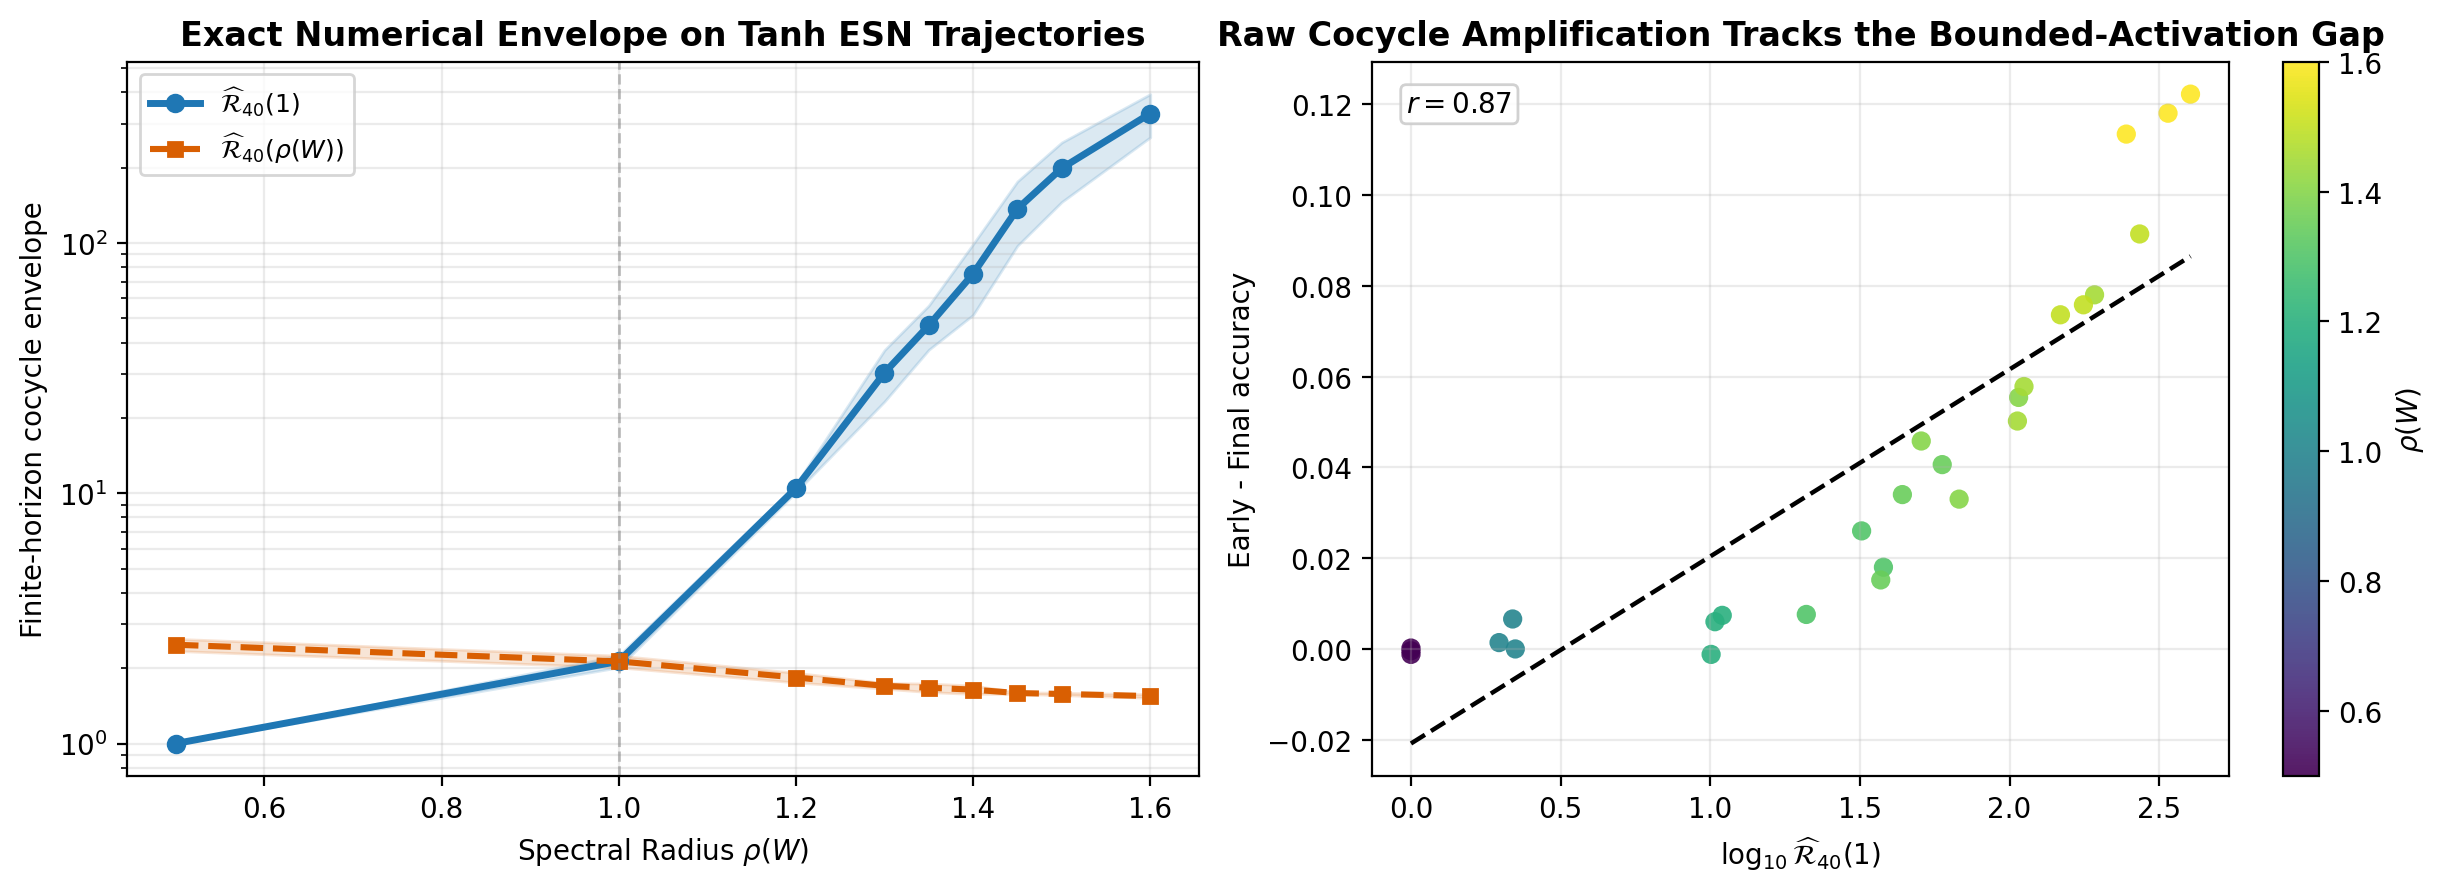
\includegraphics[width=0.82\linewidth]{fig11_cocycle_envelope}
  \caption{\textbf{Concrete numerical estimates of the cocycle envelope on the
  tanh ESN branch.} \emph{Left:} the raw finite-horizon envelope
  $\widehat{\mathcal{R}}_{40}(1)$ grows across the real-ESN sweep, while the
  scaled envelope $\widehat{\mathcal{R}}_{40}(\rho(\bW))$ remains $O(1)$ and
  gently decreases. Shading shows $\pm 1$ std across three seeds.
  \emph{Right:} $\log_{10}\widehat{\mathcal{R}}_{40}(1)$ correlates with the
  Early$-$Final gap across all $27$ tanh runs ($r=0.87$), with positive
  within-radius residual correlation ($r=0.79$).}
  \label{fig:cocycle_envelope_numeric}
\end{figure}

Proposition~\ref{prop:margin_remainder} is the frozen-Jacobian special case of
\Cref{cor:cocycle_margin}, with
$\mathcal{R}_t(\rho_\ast) \le e d\,K_{\rho_\ast}(J_\ast)$. A full nonlinear
pseudospectral theorem would require computable lifted-resolvent or
output-weighted pseudospectral bounds for
$\mathcal{T}_{i,t}^{(\lambda)}$; here we evaluate $\mathcal{R}_t(\lambda)$
directly on the bounded tanh branch and use the simpler frozen-radial proxy for
the main complex-modReLU sweep.

% =============================================================================
% BROADER IMPACT (supplementary discussion)
% =============================================================================

\section*{Broader Impact (Supplementary)}

This work studies when terminal representations degrade while usable prefixes
remain. Better readout timing could improve reliability in iterative and
physical computing, including analog reservoirs and photonic circuits.
A potential downside is deploying trajectory-aware stopping heuristics without
calibration in safety-relevant settings. For example, a photonic inference
accelerator could stop early and appear confident even though its trajectory
has left the calibrated regime, masking silent degradation. These methods are
diagnostics, not deployment guarantees; reliable use requires checking the
proxy against task accuracy in the target operating conditions.

% =============================================================================
% The NeurIPS checklist is retained in checklist.tex for the conference version.
% It is omitted from the arXiv preprint.
% =============================================================================

\end{document}
